% !TEX encoding = UTF-8 Unicode

%
% Exemple de rapport
% par Pierre Tremblay, Universite Laval
% modifié par Christian Gagne, Universite Laval
% modifié par Francis Valois, Université Laval
% 31/01/2011 - version 1.4
%

%
% Modele d'organisation d'un projet LaTeX 
% rapport/      dossier racine et fichier principal
% rapport/fig   fichiers des figures
% rapport/tex   autres fichiers .tex
%

% ** Preambule **
%
% Ajouter les options au besoin :
%    - "ULlof" pour inclure la liste des figures, requis si "\begin{figure}" utilise
%    - "ULlot" pour inclure la liste des tableaux, requis si "\begin{table}" utilise
%
\documentclass[12pt,ULlof,ULlot]{ULrapport}

% Chargement des packages supplementaires (si absent de la classe)
\usepackage[utf8]{inputenc}
\usepackage[T1]{fontenc}
\usepackage[autolanguage]{numprint}
\usepackage{icomma}
\usepackage{subfigure}
\usepackage{graphicx}
\usepackage[absolute]{textpos}
\usepackage[final]{pdfpages}
\usepackage[onehalfspacing]{setspace}
\usepackage[framed,numbered,autolinebreaks,useliterate]{mcode}
\def\dbar{{\mathchar'26\mkern-12mu d}}
\usepackage{titlesec}
\setlength\aftertitleunit{\baselineskip}

\titleformat{\chapter}[display]
  {\normalfont\Huge \scshape}{\titlerule}{-38pt}{\Huge}[\vspace{-2pt}\titlerule]
\titleformat{name=\chapter,numberless}[display]
  {\normalfont\Huge \scshape}{\titlerule}{-38pt}{\Huge}[\vspace{-2pt}\titlerule]
\titlespacing*{\chapter}{0pt}{0pt}{*2} 
%\usepackage[options]{nom_du_package}

% Definition d'une commande pour presenter des cellules multilignes dans un tableau
\newcommand{\cellulemultiligne}[1]{\begin{tabular}{@{}c@{}}#1\end{tabular}}


% Definition de colonnes en mode paragraphe avec alignement ajustable
% Cette definition requiert le chargement du package "array"
%    - alignement horizontal, parametre #1 : - \raggedright (aligne a gauche)
%                                            - \centering (c\item $K_D = 14.70$entre)
%                                            - \raggedleft (aligne a droite)
%    - alignement vertical, parametre #2 : - p (aligne en haut)
%                                          - m (centre)
%                                          - b (aligne en bas)
%    - largeur, parametre #3 : longueur
\newcolumntype{Z}[3]{>{#1\hspace{0pt}\arraybackslash}#2{#3}}

% Definitions des parametres de la page titre
\TitreProjet{Simulation d’une alimentation des électroaimants d’un accélérateur de particules. }                         % Titre du projet
\TitreRapport{Design IV - GEL-3005}       % Titre du rapport
\Destinataire{M. Robert Bergevin et M. Jérôme Cros}         % Nom(s) du destinataire
\TableauMembres{%           
   910\,010\,418  & Gabriel Boivin-Desjardins \\\hline                          % Tableau des membres de l'equipe
   910\,055\,897  & Daniel Thibodeau \\\hline
   910\,097\,879  & Francis Valois \\\hline        % matricule & nom & \\\hline
           % matricule & nom & \\\hline     % matricule & nom & \\\hline
}
\DateRemise{XX XXX 2014}                           % Date de remis


% Corps du document

\begin{document}
\tableofcontents
\listoffigures
%   Chapitres

%!TEX root = ../rapport.tex
%!TEX encoding = UTF-8 Unicode

% Chapitres "Introduction"

% modifié par Francis Valois, Université Laval
% 31/01/2011 - version 1.0 - Création du document

\chapter{Modélisation de l'alimentation électronique}
\section{Fonctionnement d'un redresseur monophasé simple alternance}
Cette section a pour objectif de décortiquer le fonctionnement d'un redresseur monophasé simple composé d'une source de courant sinusoïdale parfaite, d'un interrupteur de type IGBT et d'une charge quelconque. Le montage analysé est présenté à la figure\ref{fig:RedresseurMonophaseSimpleAlternanceIGBT}. Pour les besoins de l'exemple, une charge $RL$ théorique sera utilisée. La résistance est dénotée par $R$ et l'inductance par $L$. De plus, on suppose que l'interrupteur IGBT entre en conduction lorsqu'un échelon de tension unitaire est appliqué à la grille de celui-ci, on le modélise comme un interrupteur idéal. Finalement, en supposant des modèles sans pertes, l'équation de circuit se résume à celle présentée à l'équation \ref{eq:RLSimple}. À noter que l'échelon unitaire est défini comme: $u(t<0) = 0, u(t\geq 0) = 1)$.

\begin{figure}[htb!]
	\begin{center}  
		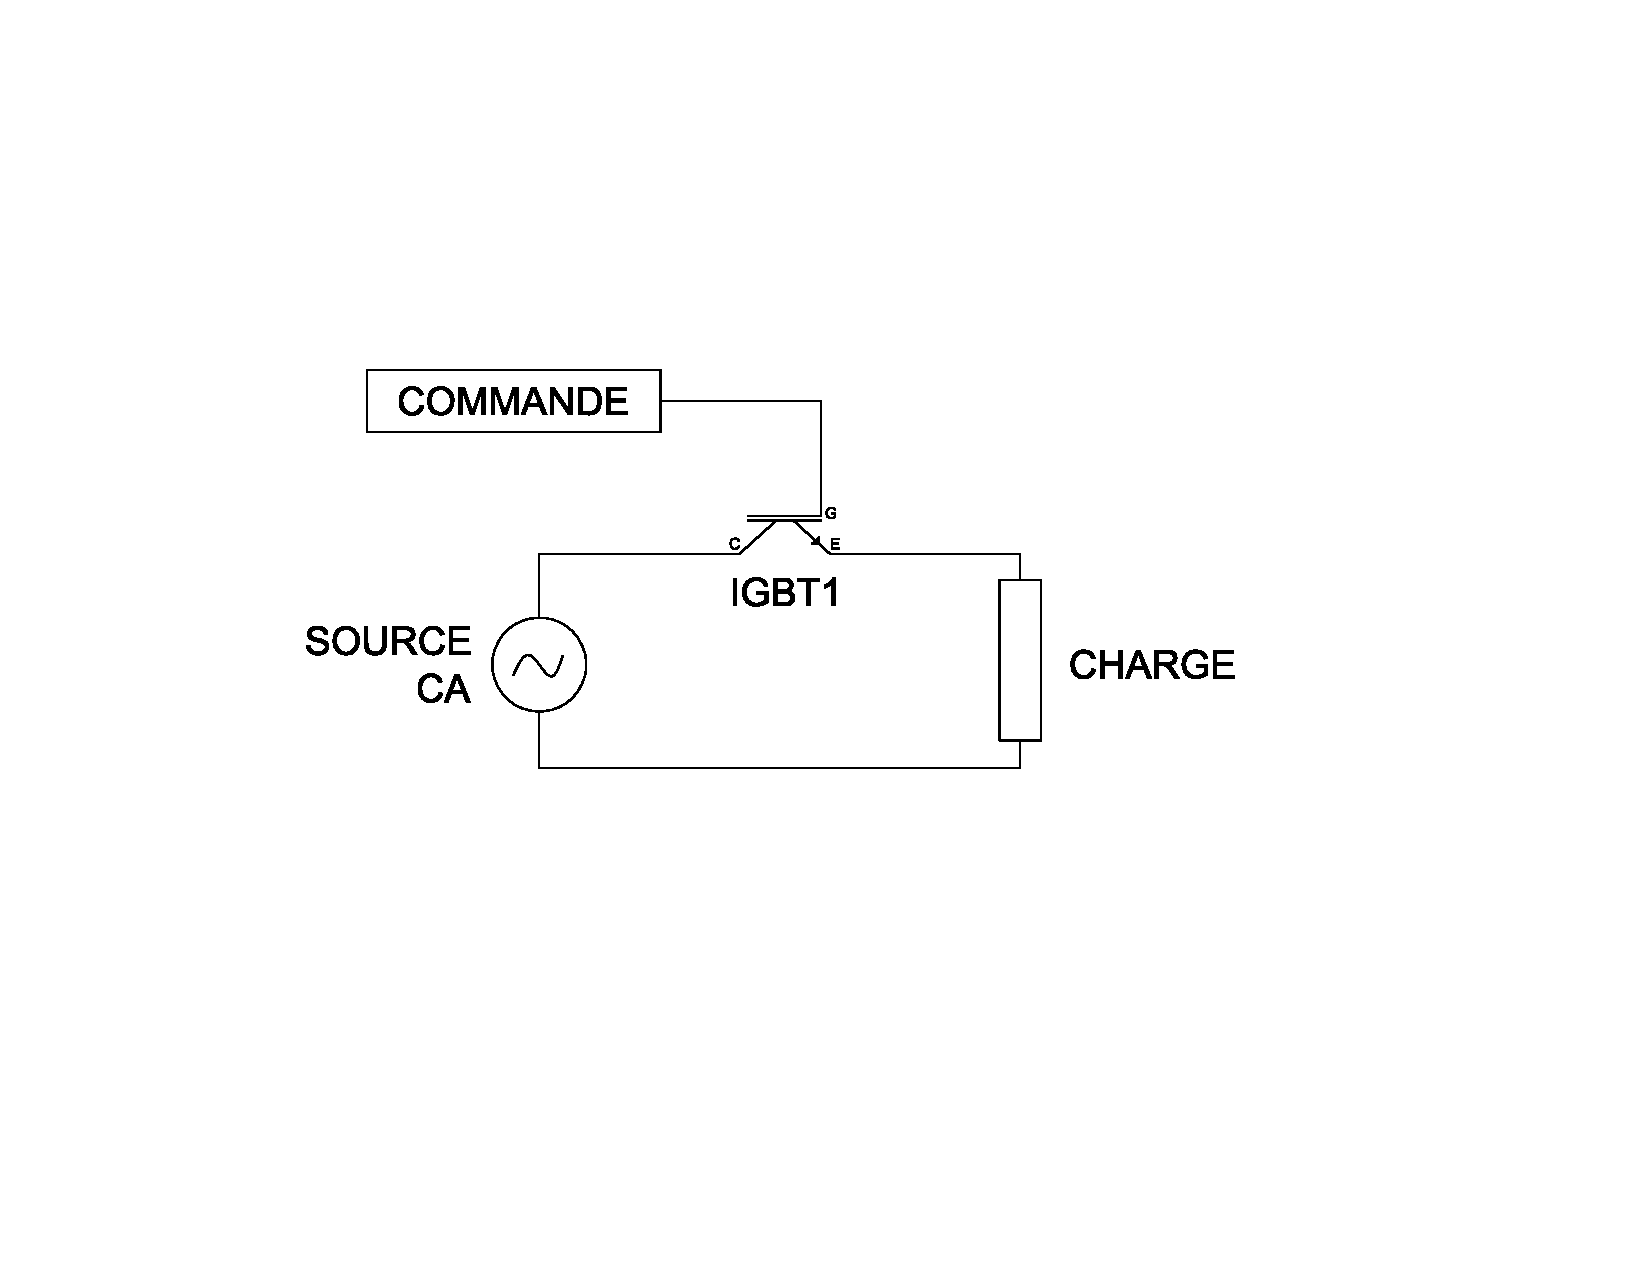
\includegraphics[width=0.7\textwidth]{Circuit/RedresseurMonophaseSimpleAlternanceIGBT}
		\caption{Circuit redresseur monophasé simple alternance avec IGBT et charge quelquonque}
		\label{fig:RedresseurMonophaseSimpleAlternanceIGBT}
	\end{center}   
\end{figure}


\begin{equation}
\label{eq:RLSimple}
v(t) = R i(t) + L \frac{d i(t)}{dt}
\end{equation}

Si l'on suppose la conduction continue de l'IGBT, il est possible d'exprimer le courant dans la charge en fonction de la tension de la source CA:

\begin{eqnarray}
V_{in}(t) &=& E_m\sin{\omega_0 t} \\
|Z| &=& \sqrt{R^2 + (\omega_0 L)^2} \\
\tau &=& \frac{L}{R}\\
\phi &=& \mbox{atan}(\omega_0 \tau) = \mbox{atan}(\omega_0 \frac{L}{R}) \\
\label{eq:solutionRLSimple} i(t) &=& \frac{E_m\sin{\phi}}{|Z|}\mbox{e}^{\frac{-t}{\tau}} + \frac{E_m\sin{(\omega_0 t + \phi})}{|Z|}\\
i(t=0) &=& i_0\\
i(t) &=& i_0  + \frac{E_m\sin{\phi}}{|Z|}\mbox{e}^{\frac{-t}{\tau}} + \frac{E_m\sin{(\omega_0 t + \phi})}{|Z|} \\
\end{eqnarray}

L'équation \ref{eq:solutionRLSimple} est la solution de l'équation différentielle \ref{eq:RLSimple} d'un circuit RL avec la partie de gauche qui est la solution transitoire (dépendante du circuit seulement) et la partie de droite qui est la solution en régime permanent (dépendante de l'excitation). 

\paragraph{}
La fonction principale de ce redresseur est de produire une tension et un courant qui sont strictement positifs. Dans le cas du redresseur simple alternance, seulement la partie positive de la source de courant alternative est envoyé à la charge et la partie négative est bloquée par l'IGBT qui agit comme une diode. De plus, du fait que l'IGBT est une source de courant commandée (sans pertes et sans délais pour les calculs théoriques) , il est possible de contrôler le temps de conduction de la partie positive du signal.

Ainsi, si l'on définit le temps total d'une période du signal par $T$, le temps de début de conduction de l'IGBT par $t_{on}$ et le temps de début de blocage par $t_{off}$, il est possible de définir le rapport de modulation $m = 2\cdot \frac{t_{off}-t_{on}}{T}$. Supposons un rapport de modulation $m_x$, il est possible, si l'on considère le courant initial nul et des temps de commutation nuls, d'exprimer le courant dans la charge RL pour une période $T$ donnée.

Les figures \ref{fig:RedresseurMonophaseSimpleAlternanceIGBTCourbes50} et \ref{fig:RedresseurMonophaseSimpleAlternanceIGBTCourbes100} présentent la tension et le courant dans la charge pour 2 différents niveaux de modulation. 

\begin{figure}
        \centering       
        \begin{subfigure}[Courant dans la charge en fonction de la tension dans la charge pour une modulation de 50\% avec un temps de début de conduction de 10\%]{
         		\label{fig:RedresseurMonophaseSimpleAlternanceIGBTCourbes50}
                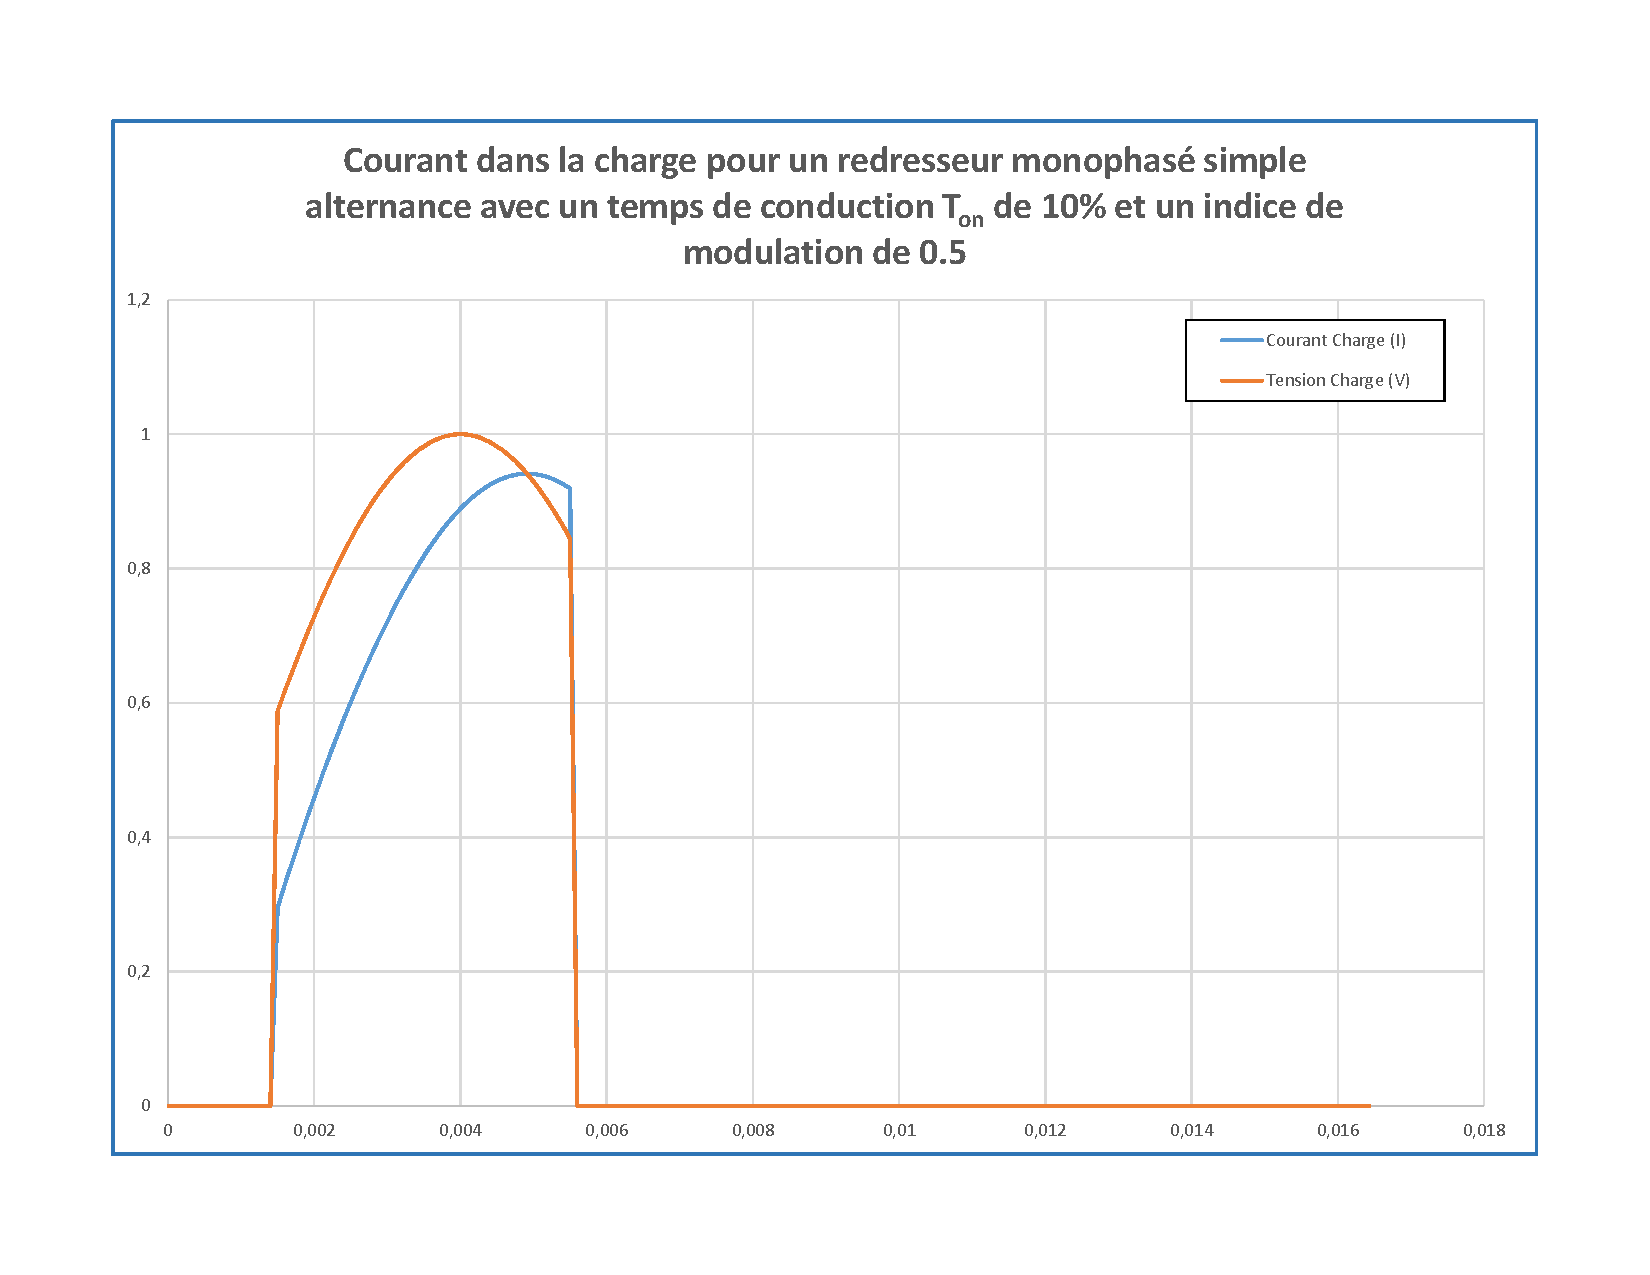
\includegraphics[width=0.68\textwidth]{Graphs/RedresseurMonophaseSimpleAlternance50}}
        \end{subfigure}        
        \begin{subfigure}[Courant dans la charge en fonction de la tension dans la charge pour une modulation de 100\% avec un temps de début de conduction de 0\%]{
         		\label{fig:RedresseurMonophaseSimpleAlternanceIGBTCourbes100}
                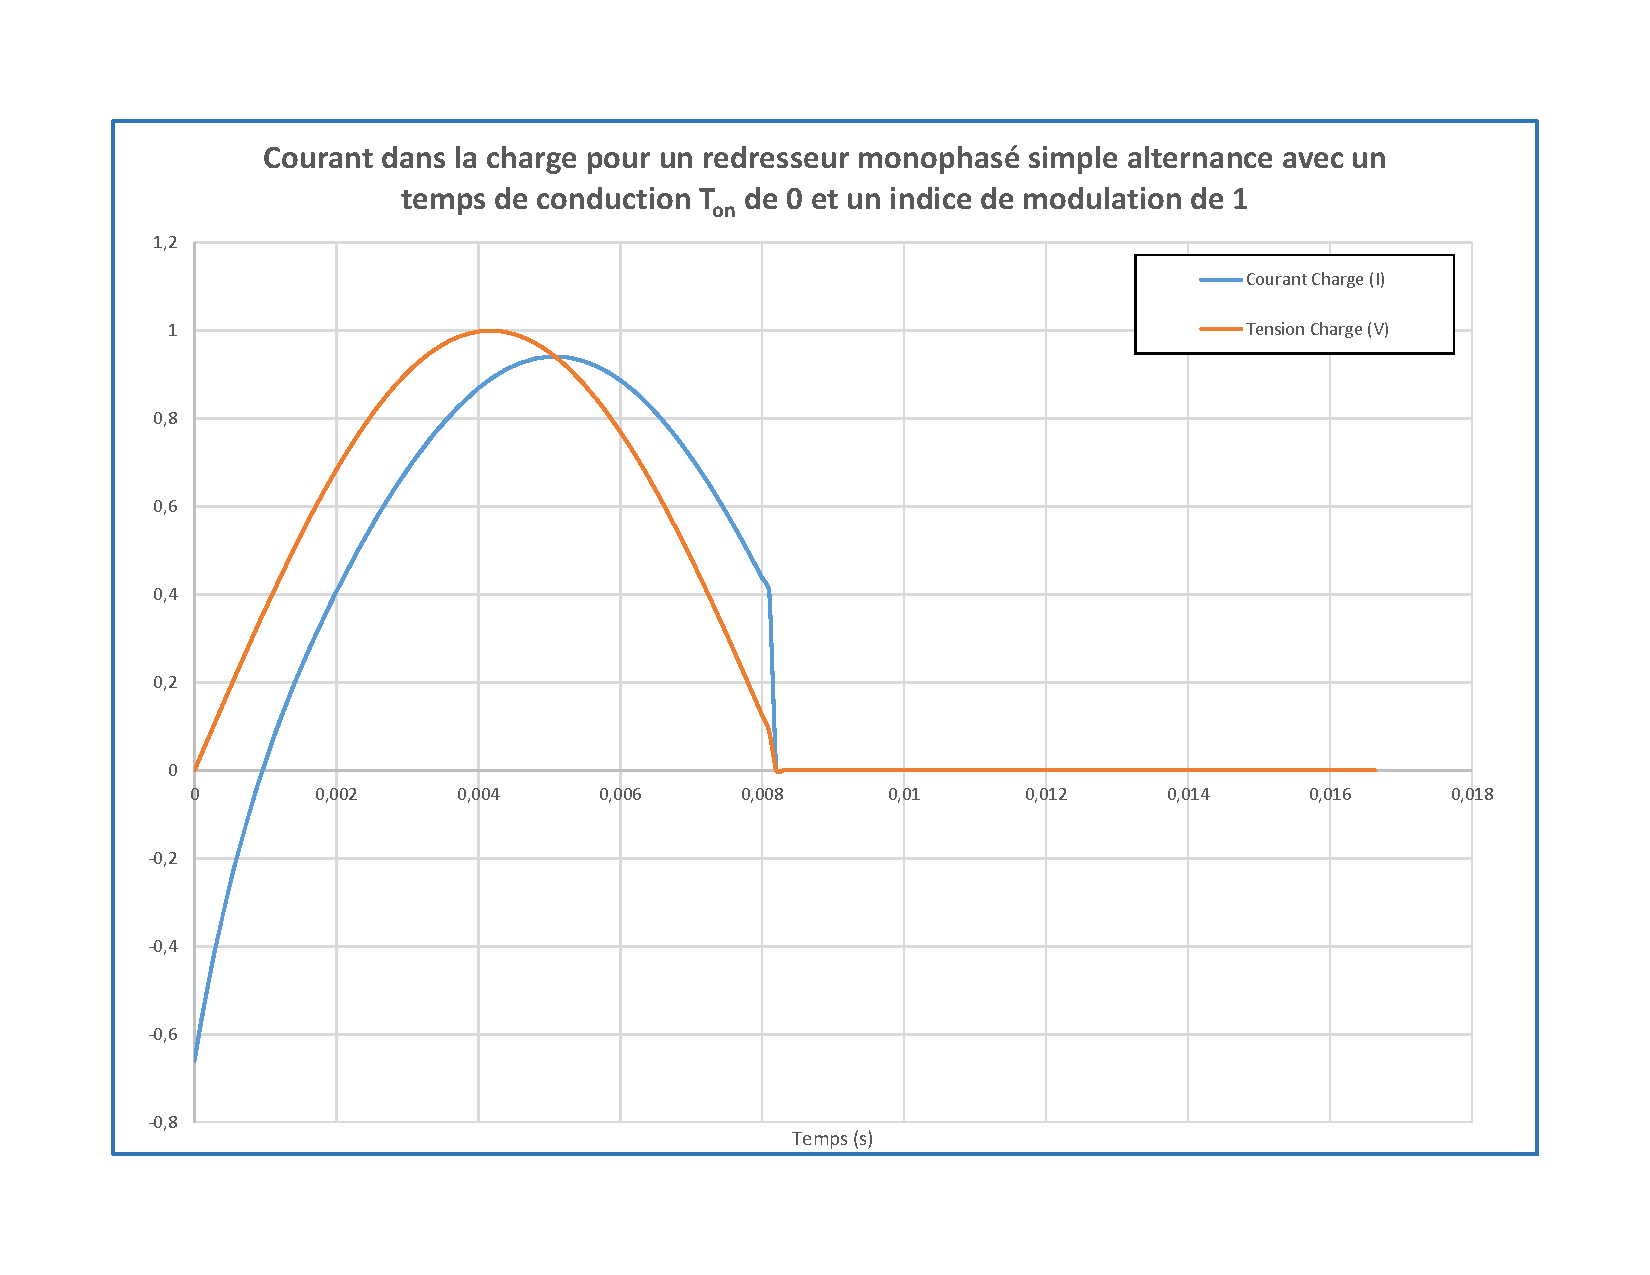
\includegraphics[width=0.68\textwidth]{Graphs/RedresseurMonophaseSimpleAlternance100}}
        \end{subfigure}
        \caption{Forme du courant et de la tension dans la charge pour 2 différents niveaux de modulation du redresseur monophasé à simple alternance}\label{fig:RedresseurMonophaseSimpleAlternanceIGBTCourbes}
\end{figure}

Comme la forme d'onde de tension et de courant dépendent entièrement du niveau de modulation choisi, il est intéressant d'obtenir les valeurs de tension et de courant moyen en fonction des paramètres de modulation. La valeur moyenne du courant sur une période se calcule comme suit :

\begin{eqnarray}
I_{moy} &=& \frac{1}{T}\int_{t_{on}}^{t_{off}} i(t) dt \\
I_{moy} &=& \frac{1}{T}\int_{t_{on}}^{t_{off}} \left( \frac{E_m\sin{\phi}}{|Z|}\mbox{e}^{\frac{-t}{\tau}} + \frac{E_m\sin{(\omega_0 t + \phi})}{|Z|}\right) dt \\
I_{moy} &=& \frac{E_m}{T} \left( \frac{-\mbox{e}^{-\frac{t_{off}}{\tau}}\sin{(\phi)}\omega_0 \tau + \mbox{e}^{-\frac{t_{on}}{\tau}} + \cos{(\omega_0 t_{on} + \phi)}-\cos{(\omega_0 t_{off} + \phi)}}{|Z|\omega_0} \right)
\end{eqnarray}

Par la suite, la valeur moyenne de la tension se calcule comme suit : 
\begin{eqnarray}
V_{moy} &=& \frac{1}{T}\int_{t_{on}}^{t_{off}} V_{in}(t) dt \\
V_{moy} &=& \frac{1}{T}\int_{t_{on}}^{t_{off}} (E_m \sin{\omega_0 t}) dt \\
V_{moy} &=& \frac{E_m}{T} \left( \frac{\cos{(\omega_0 t_{on})} - \cos{(\omega_0 t_{off})}}{\omega_0} \right)
\end{eqnarray}

\section{Fonctionnement d'un redresseur monophasé double alternance}
Cette section a pour objectif de décortiquer le fonctionnement d'un redresseur monophasé à double alternance réversible en courant et en tension, composé d'une source de courant sinusoïdale parfaite, de 4 interrupteurs de type IGBT (avec diodes en antiparallèle) et d'une charge quelconque. Le montage analysé est présenté à la figure à la figure \ref{fig:RedresseurMonophaseDoubleAlternanceIGBT}. Le principal avantage de ce type de redresseur par rapport au redresseur simple alternance est la possibilité d'inverser la partie négative du signal alternatif et de permettre la réversibilité en courant et en tension. En effet, lors de la partie positive de l'onde, les IGBT 1 et 3 vont s'activer ce qui va permettre d'alimenter la charge avec une tension positive et lors de la partie négative de l'onde, les IGBT 2 et 4 vont conduire et ainsi alimenter la charge avec une tension redressée. 

\begin{figure}[htb!]
  \begin{center}  
    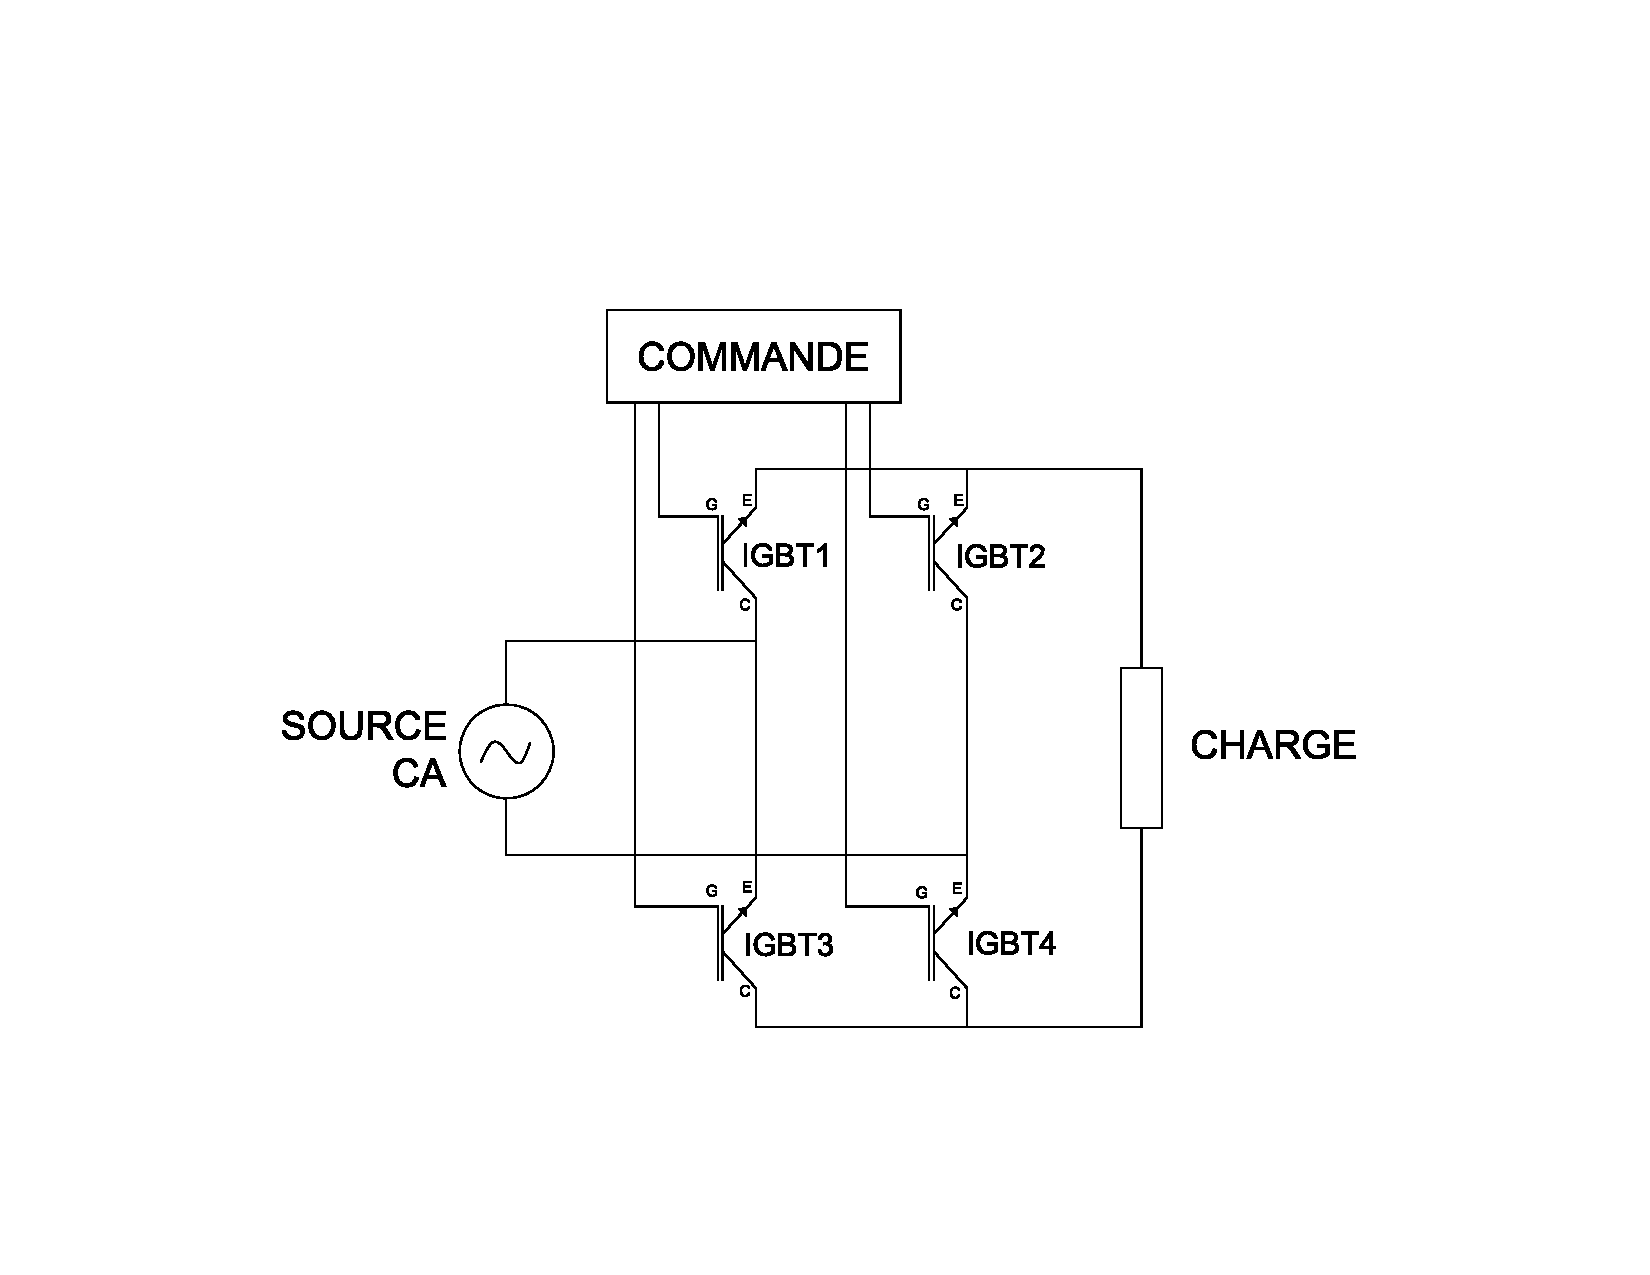
\includegraphics[width=0.7\textwidth]{Circuit/RedresseurMonophaseDoubleAlternanceIGBT}
    \caption{Circuit redresseur monophasé double alternance avec IGBT et charge quelquonque}
    \label{fig:RedresseurMonophaseDoubleAlternanceIGBT}
  \end{center}   
\end{figure}

\paragraph{}
La présence de l'alternance négative redressée permet deux modes de conduction, soit le mode continu et le mode discontinu. Comme les équations du système en régime permanent sont différentes dans les deux modes, il est nécessaire d'effectuer la résolution pour les deux différents cas.

\subsection{Mode continu}
Le redresseur double alternange opère dans le mode continu lorsque le courant dans la charge ne retombe jamais à zero. Ainsi, il est nécessaire d'adapter l'équation \ref{eq:solutionRLSimple} trouvée dans la section précédente. Nous savons que le courant dans la charge RL, une fois l'inductance chargée, est donné par :

\begin{eqnarray}
\label{eq:RedresseurMonophaseDoubleAlternanceContinu1}
i(t) &=& C_1\mbox{e}^{\frac{-t}{\tau}} + \frac{E_m\sin{(\omega_0 t - \phi})}{|Z|}
\end{eqnarray}

Où:
\begin{eqnarray}
C_1 &=& \left( I_1 - \frac{E_m\sin{(\omega_0 t + \phi})}{|Z|}\right)\mbox{e}^{\left(\frac{R}{L}\right)\left(\frac{\pi}{\omega_0}\right)}
\end{eqnarray}

En appliquant la condition $I_L(\omega_0 t = 0)=I_L(\omega_0 t=\pi)=I_1$ dans l'équation \ref{eq:RedresseurMonophaseDoubleAlternanceContinu1}, nous trouvons que :
\begin{equation}
\label{eq:RedresseurMonophaseDoubleAlternanceContinu2}
	I_1 = \frac{E_m\sin{(\phi)}}{|Z|}  \frac{1 + \mbox{e}^{\frac{-1}{\tau}}}{1 - \mbox{e}^{\frac{-1}{\tau}}}
\end{equation}

Finalement en remplaçant $I_1$ dans l'équation \ref{eq:RedresseurMonophaseDoubleAlternanceContinu1} par l'équation \ref{eq:RedresseurMonophaseDoubleAlternanceContinu2}, nous trouvons que le courant dans la charge pour chaque demi-période, une fois l'inductance chargée, est donné par :

\begin{equation}
	i(t) = \frac{E_m}{|Z|}\left[\sin{(\omega_0 t - \phi)} + \frac{2\sin(\phi) \mbox{e}^{\frac{-t}{\tau}}}{1-\mbox{e}^{\left(\frac{R}{L}\right)\left(\frac{\pi}{\omega_0}\right)}} \right] 
\end{equation}

\subsection{Mode discontinu}
Le redresseur double alternange opère dans le mode discontinu lorsque le courant dans la charge peut retomber à zero. Ainsi, il est nécessaire d'adapter l'équation \ref{eq:solutionRLSimple} trouvée dans la section précédente. Nous savons que le courant dans la charge RL ,une fois l'inductance chargée, est donné par :

\begin{eqnarray}
\label{eq:RedresseurMonophaseDoubleAlternanceContinu1}
i(t) &=& C_1\mbox{e}^{\frac{-t}{\tau}} + \frac{E_m\sin{(\omega_0 t - \phi})}{|Z|}
\end{eqnarray}

Où:
\begin{eqnarray}
C_1 &=& \left( I_1 - \frac{E_m\sin{(\omega_0 t + \phi})}{|Z|}\right)\mbox{e}^{\left(\frac{R}{L}\right)\left(\frac{\pi}{\omega_0}\right)}
\end{eqnarray}

En appliquant la condition $I_L(\omega_0 t = 0)=I_L(\omega_0 t=\pi)=I_1$ dans l'équation \ref{eq:RedresseurMonophaseDoubleAlternanceContinu1}, nous trouvons que :
\begin{equation}
\label{eq:RedresseurMonophaseDoubleAlternanceContinu2}
	I_1 = \frac{E_m\sin{(\phi)}}{|Z|}  \frac{1 + \mbox{e}^{\frac{-1}{\tau}}}{1 - \mbox{e}^{\frac{-1}{\tau}}}
\end{equation}

Finalement en remplaçant $I_1$ dans l'équation \ref{eq:RedresseurMonophaseDoubleAlternanceContinu1} par l'équation \ref{eq:RedresseurMonophaseDoubleAlternanceContinu2}, nous trouvons que le courant dans la charge pour chaque demi-période, une fois l'inductance chargée, est donné par :

\begin{equation}
	i(t) = \frac{E_m}{|Z|}\left[\sin{(\omega_0 t - \phi)} + \frac{2\sin(\phi) \mbox{e}^{\frac{-t}{\tau}}}{1-\mbox{e}^{\left(\frac{R}{L}\right)\left(\frac{\pi}{\omega_0}\right)}} \right] 
\end{equation}

\section{Fonctionnement d'un redresseur triphasé double alternance}
Cette section a pour objectif de décortiquer le fonctionnement d'un redresseur triphasé à double alternance réversible en courant et en tension, composé de 3 sources de courant sinusoïdale parfaites, de 6 interrupteurs de type IGBT(avec diodes en antiparallèle) et d'une charge quelconque. Le montage analysé est présenté à la figure à la figure \ref{circuit_AFE_2L_RC}. Ce montage est analogue à celui présenté à la section précédente et permet de diminuer l'ondulation vue à la charge. Il est réversible en courant et en tension, tout comme le montage précédent. Seule l'utilisation en régime permanent (régulation de tension) sera présentée dans ce document, le développement mathématique utile pour la compréhension fondamentale ayant été présenté plus tôt. Dans cet exemple, on suppose une charge $RC$, dont la résistance correspond à la valeur nominale de la puissance moyenne débitée par le redresseur. Si l'on suppose un condensateur C, initialement chargé à une tension désirée, une source de courant parfaite côté réseau, des commutations instantanées et sans pertes et que l'on néglige les snubbers, il est possible de dresser un portrait mathématique simple du redresseur. La fonction de transfert d'un circuit $RC$ dans le domaine de Laplace est donnée par l'équation suivant:
\begin{equation}
H(s) = \frac{R}{RCs + 1}
\end{equation}
Il est possible de supposer que le courant injecté par chaque bras du redresseur dans la charge est modulable selon le temps de conduction de l'IGBT concerné selon la phase du signal par rapport aux autres (seul le montage dont la tension est supérieure (en valeur absolue) aux autres s'amorce. La période de conduction totale et maximale d'un IGBT est de 60 degrés, sur une période totale de 360 degrés. Pour simplifier l'analyse, on peut analyser le montage comme 6 montages redresseurs monophasés simple alternance et ne se concentrer que sur un IGBT. Par ailleurs, on peut négliger l'ondulation liée à la nature sinusoïdale de la charge et approximer par la valeur moyenne d'un sinus sur cette période, que l'on calcule comme suit (fonctionnement pleine onde):
\begin{equation}
I_{moy} = \frac{3}{\pi}\int_{60}^{120} I_M \sin(\theta)d\theta = \frac{3I_M}{\pi}\left( \cos(60)-\cos(120)\right) = \frac{3I_M}{\pi}
\end{equation}
On trouve par la suite que selon l'indice de modulation ($m_x$) sur la période de 60 degrés donnée et ce, pour une fréquence de modulation de $f_{mod} = \frac{1}{T_{mod}}$ on peut approximer le courant dans la charge par $I_{CH} = \frac{3I_M m_x}{pi}$. Pour le reste de la période de modulation, on a 0A. Pour une période de modulation, la tension vue à la charge est donnée par l'équation suivante dans le domaine de Laplace:
\begin{equation}
V(s) = \frac{R\cdot I_{CH}}{RCs + 1} \left(\frac{1 - e^{-m_xT_{mod}s}}{s}\right) = R\cdot I_{CH}\frac{1/RC}{s(s + 1/RC)} - R\cdot I_{CH}\frac{1/RC}{s(s + 1/RC)}e^{-m_xT_{mod}s}
\end{equation}
On peut par la suite effectuer la transformation dans le domaine du temps en supposant qu'on applique un courant à un moment quelconque
\begin{equation}
v(t) = R\cdot I_{CH}\left((1-e^{-(t-t_0)/RC})u(t-t_0) - (1-e^{t-(m_xT_{mod}-t_0)/RC})u(t-m_xT_{mod}-t_0)\right) + v_C(t_0)
\end{equation}
Pour une période de conduction de 60$^\circ$, donc de 3.33ms à 50Hz et un temps de modulation de 1ms, il est possible de calculer le courant dans un interrupteur. On sait premièrement que la puissance nominale du montage étudié est de 2.7MW à 5000V. On calcule donc une résistance équivalente R étant égale à 9.26$\Omega$ et un courant DC moyen de 540A à la charge. Le banc de condensateurs est fixe à 330mF. On suppose que l'origine du temps est à 0s. Connaissant la forme de la tension à la charge, il est possible de déterminer le courant traversant la résistance en fonction du temps si l'on considère une source de courant idéale à l'entrée:
\begin{equation}
i_R(t) = I_{CH}(1-e^{-(t)/RC})u(t) - I_{CH}(1-e^{t-(m_xT_{mod})/RC})u(t-m_xT_{mod}) + v_C(0)/R
\end{equation}
On considère maintenant le système en régime permanent et on cherche  à ce que l'indice de modulation soit tel que la moyenne du courant soit le courant nominal. Le courant de source crête est égal à $I_M = \sqrt(2/3)V_{AC} = 2000\sqrt{2/3} = 1633A$ et donc le courant moyen de charge égal à $I_{CH} = \frac{3I_M m_x}{pi} = \frac{2000\sqrt(6)m_x}{\pi} = 1559.39m_xA$. On désire un courant moyen dans la charge de 540A. , il est alors nécessaire que l'indice de modulation soit de 0.346. 
Par ailleurs, le redresseur est en mesure de fournir jusqu'à 3.6MW de puissance crête et ce, au moment où la tension du bus CC chute à environ 3.2kV. On peut donc calculer l'indice de modulation à cette puissance de la même manière que précédemment et on obtient 0.721, soit un courant moyen de 1125A à la charge. Il est à noter qu'en pratique on régule l'amplitude du courant côté réseau en imposant une référence de courant d'amplitude variable qui permet d'imposer l'indice de modulation approprié.

Dans le cas où la puissance demandée est maximale, il est possible de calculer une approximation des valeurs de courants RMS vues par les interrupteurs et de les comparer à celles prévues par le manufacturier. On a premièrement que le courant maximal (en valeur moyenne) débité par la source idéale (côté réseau) est de 1559.39A. Il est possible de calculer la valeur RMS maximale sur la période de conduction d'un IGBT en connaissant l'indice de modulation. Soit $m_x = 0.721$, on a que:

\begin{equation}
I_{RMS} = \sqrt{\int_0^{m_x} I_{CH}^2} = \sqrt{m_x}I_{CH}  \sqrt{0.721}I_{CH}= 1324A
\end{equation}

Sur l'ensemble d'une période du signal, on a donc:
\begin{equation}
I_{RMS} =  \sqrt{1/6\int_0^{m_x} I_{CH}^2} = \frac{1}{\sqrt{6}}\cdot 1324A = 540.52A
\end{equation}

En fonctionnement à puissance nominale, on trouve que le courant RMS pendant la conduction est donné par:
\begin{equation}
I_{RMS} =  \sqrt{m_x}I_{CH} = \sqrt{0.346}I_{CH} = 917.26A
\end{equation}

Sur l'ensemble d'une période du signal, on a donc:
\begin{equation}
I_{RMS} =  \sqrt{1/6\int_0^{m_x} I_{CH}^2} = \frac{1}{\sqrt{6}}\cdot 917.26A = 374.47A.
\end{equation}

Il est aussi possible d'extraire directement la forme de tension du BUS CC et d'utiliser la puissance moyenne dissipée dans les électroaimants afin de dimensionner les interrupteurs. À puissance crête nous avons déterminé que le courant maximal RMS que doivent pouvoir commuter les interrupteurs est de l'ordre de 1324A. En fonctionnement normal, la documentation technique du CERN évalue la puissance moyenne dissipée sur 0.9s (un cycle) à 2.25MW. Soit la courbe de la tension moyenne du bus CC en fonction du temps pour un cycle donné, présenté à la figure \ref{fig_Tension_BUSCC}, il est possible de déterminer le courant moyen en fonction du temps si l'on suppose une puissance constante de 2.25MW. Il est par la suite possible de calculer la valeur RMS de ce courant. Cette valeur RMS nous donne 490A, elle est calculée en utilisant la puissance constante de 2.25MW ainsi que la tension du bus CC présentée à la figure \ref{eq:RLSimple} et en calculant la valeur RMS du courant obtenu. Avec cette valeur, on peut déterminer l'indice de modulation nécessaire. On cherche donc $m_x$, tel que $1559.39m_x = 490$. On trouve alors $m_x = 0.314$. Sur la période de conduction de l'interrupteur on a que
\begin{equation}
I_{RMS} = \sqrt{\int_0^{m_x} I_{CH}^2} = \sqrt{m_x}I_{CH}  \sqrt{0.314}I_{CH}= 873.815A
\end{equation}

Sur l'ensemble d'une période du signal, on a donc:
\begin{equation}
I_{RMS} =  \sqrt{1/6\int_0^{m_x} I_{CH}^2} = \frac{1}{\sqrt{6}}\cdot 873.815A = 356.73A
\end{equation}

Le tableau \ref{tab_Courant_AFE} présente un résumé des différentes valeurs obtenues

\begin{table}[htb]
\begin{tabular}{|c|c|c|}
\hline
\multirow{2}{*}{Puissance (MW)} & \multirow{2}{*}{Courant RMS (A) sur 60$^\circ$} & \multirow{2}{*}{Courant RMS (A) sur une période complète} \\
                                &                                                 &                                                           \\ \hline
2.25                            & 873.8                                           & 356.73                                                    \\ \hline
2.7                             & 917.26                                          & 374.47                                                    \\ \hline
3.6                             & 1324                                            & 540.52                                                    \\ \hline
\end{tabular}
\caption{Courants RMS approximatifs vus par les interrupteurs de l'AFE}
\label{tab_Courant_AFE}
\end{table}
\begin{figure}[htb]
\centering
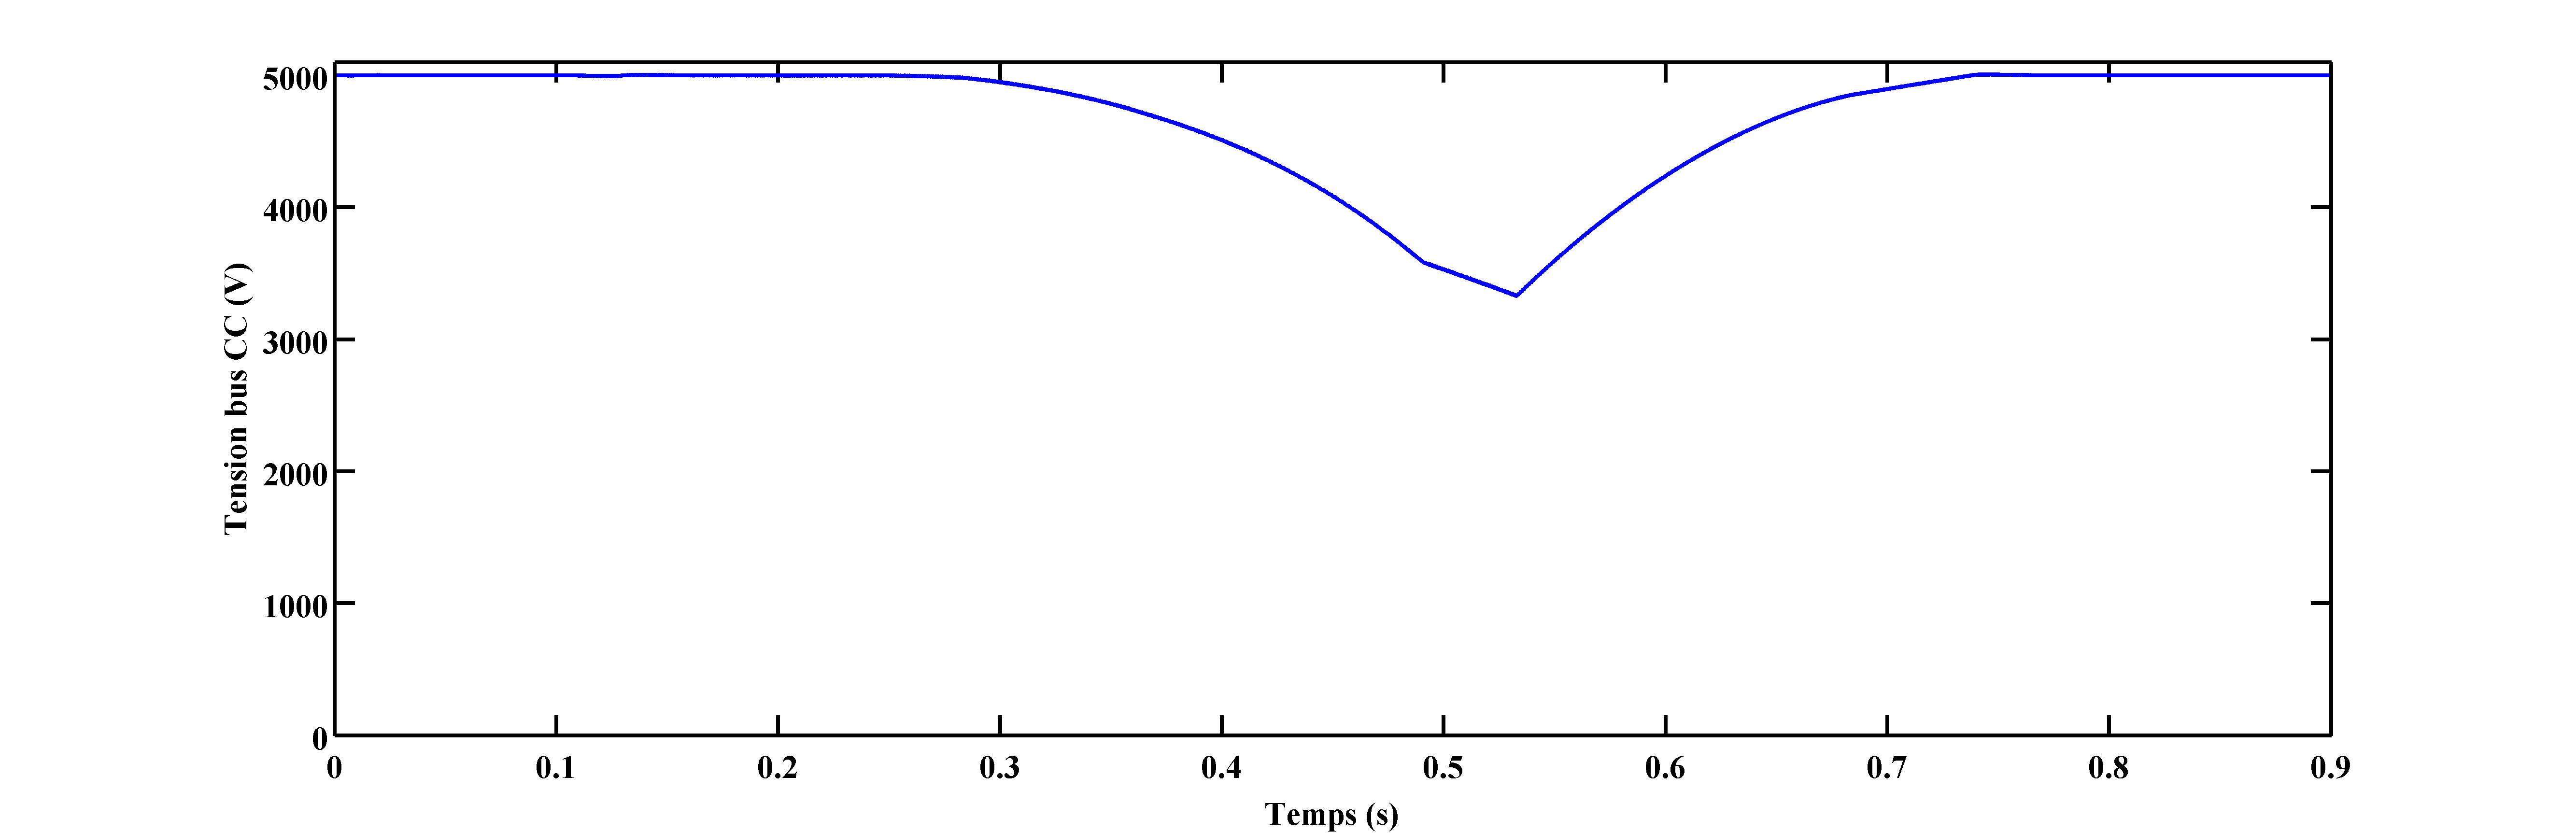
\includegraphics[scale=0.35]{fig/fig_VbusCC.png}
\caption{Tension du bus CC en fonction du temps pour un cycle du PS-Booster}
\label{fig_Tension_BUSCC}
\end{figure}
\section{Fonctionnement d'un redresseur triphasé 3 niveaux NPC}
Le projet implanté au CERN emploie un redresseur triphasé à 3 niveaux NPC dont le schéma est présenté à la figure \ref{circuit_AFE_3L_RC}. L'avantage de cette configuration par rapport à la précédente est au niveau de la tension vue aux bornes des interrupteurs. En fonctionnement normal, l'ajout d'un niveau supplémentaire divise par 2 la tension commutée par les interrupteurs, ce qui permet d'avoir des composantes de dimensions inférieures. Au point de vue logique et commande, les calculs théoriques approximatifs tiennent toujours, le fonctionnement  de base est pratiquement inchangé du point de vue du courant. Cependant, dans cette configuration, les interrupteurs conduisent par paires dans chaque bras, ce qui modifie la commande à appliquer. De plus, l'ajout d'un point milieu \og clampé \fg{} par des diodes modifie substantiellement la stabilité de la tension 0 dans cette configuration. les séquences d'enclenchement des niveaux vont perturber la tension de neutre. En pratique, cette tension doit être équilibrée par un circuit de commande auxiliaire. Aussi, il faut donc dimensionner les interrupteurs de manière à pouvoir commuter la moitiée de la tension du bus CC de  5kV, soit 2.5kV. Le bus CC pouvant monter jusqu'à 5.1kV, il est nécessaire de dimensionner les IGBT pour obtenir une tension de 2.75kV en répétition à leurs bornes.
\chapter{Modélisation du convertisseur CC-CC}
\section{Fonctionnement d'un onduleur monophasé à 2 niveaux}
L'onduleur monophasé à 2 niveaux est composé de deux IGBT. Ils correspondent à un bras d'onduleur, tel que présenté à la figure \ref{circuit_AFE_2L_RC}. Soit une charge $RL$ théorique, dont la résistance se nomme $R$ et l'inductance $L$, on constate que si l'on applique un échelon de tension à la grille de l'IGBT supérieur et que l'on considère l'IGBT comme étant sans pertes et que l'on suppose qu'il entre en saturation avec un échelon unitaire, l'équation de circuit se résume à celle présentée à l'équation \ref{eq1}. À noter que l'échelon unitaire est défini comme: $u(t<0) = 0, u(t\geq 0) = 1)$.

\begin{equation}
\label{eq1}
v(t) = R i(t) + L \frac{d i(t)}{dt}
\end{equation}

On considère que les diodes branchées en parallèle avec les IGBT servent à assurer la continuité du courant lors des commutations.Si l'on néglige la chute de tension aux bornes des IGBT et des diodes, il est possible d'exprimer le courant en fonction de la tension:

\begin{eqnarray}
v(t) &=& V_{DC} u(t)\\
i(t) &=& \frac{V_{DC}}{R} + K \mbox{e}^{\frac{-R}{L}t}\\
i(t=0) &=& i_0\\
K &=& i_0 - \frac{V_{DC}}{R} \\
i(t) &=& i_0  + \frac{V_{DC}}{R}\left(1 - \mbox{e}^{\frac{-R}{L}t}\right)u(t)
\end{eqnarray}

Si l'on définit le temps total d'une modulation par $T$, le temps de conduction de l'alternance positive par $t_{on}$ et le temps de conduction de l'alternance négative par $t_{off}$ il est possible de définir le rapport de modulation $m = \frac{t_{on}}{T} = \frac{1-t_{off}}{T}$. Supposons un rapport de modulation $m_x$, il est possible, si l'on considère le courant initial nul, d'exprimer le courant dans la charge RL pour une période de modulation étant égale à $T$. L'évolution du courant pour une tension appliquée pendant un cycle de modulation est présenté à la figure \ref{eq1}
\begin{figure}
\centering
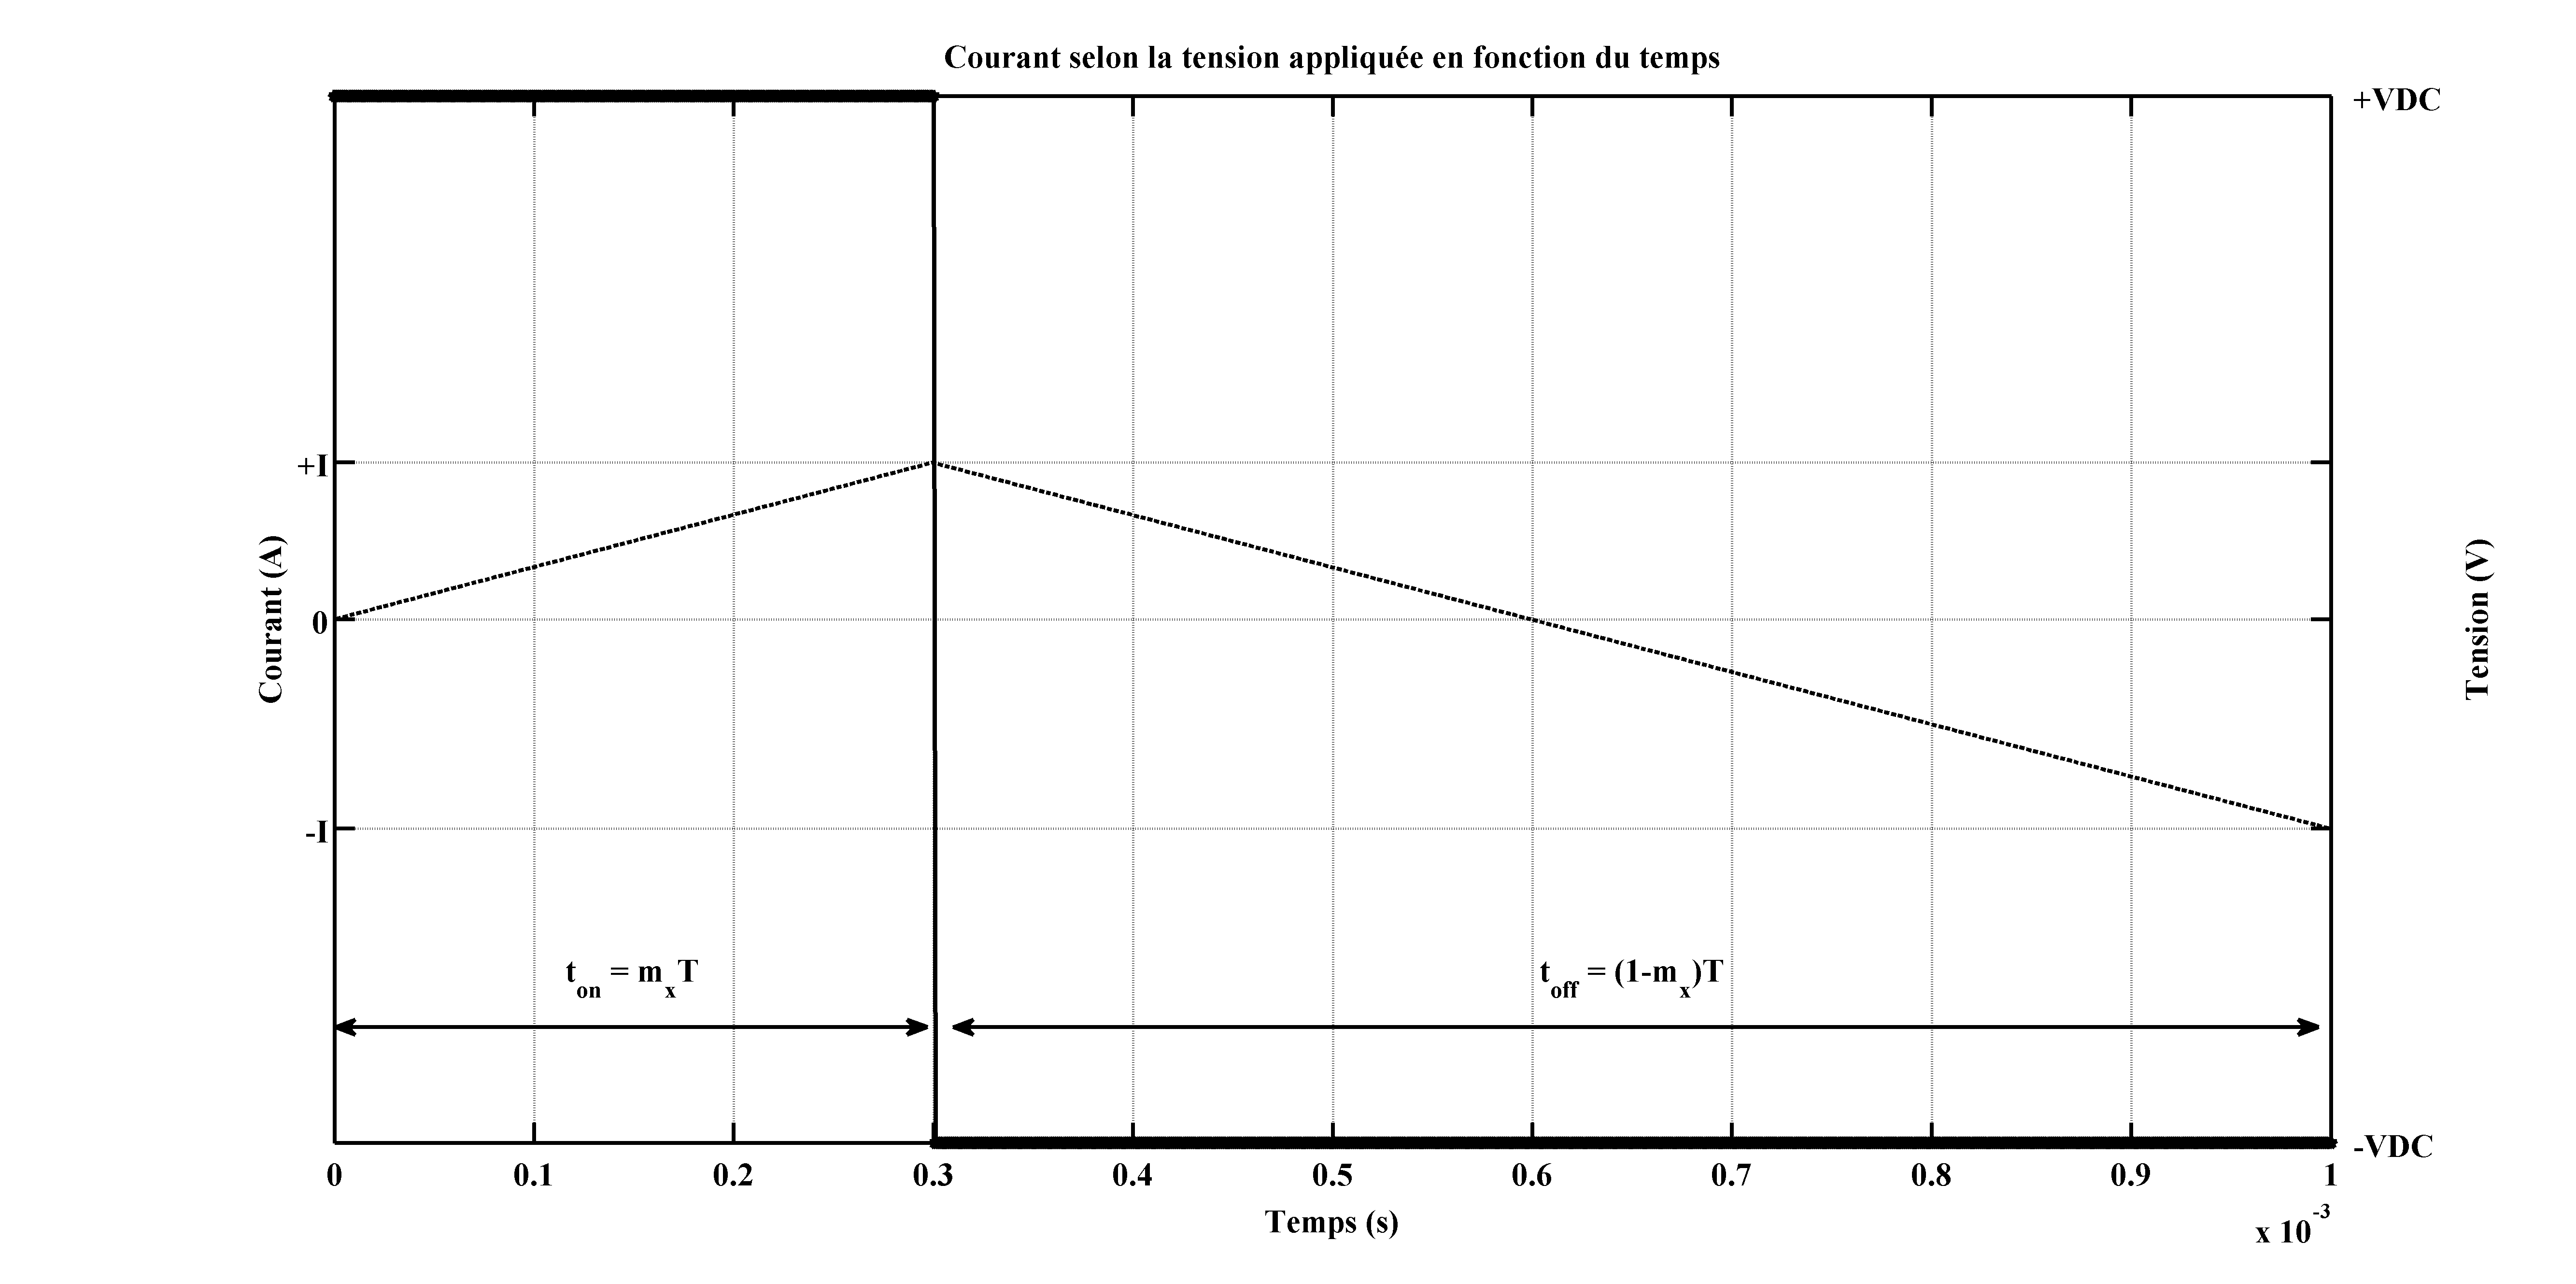
\includegraphics[scale=0.4]{fig/fig_courant_tension_mod.png}
\caption{Courant dans la charge selon une tension $+V_{DC}$ appliquée pendant un temps $t_{on}$ et une tension $-V_{DC}$ appliquée pendant un temps $t_{off}$ pour un cycle de modulation.}
\end{figure}
\begin{eqnarray}
t_{on} &=& m_x T, i_0 = 0\\
i\left(t = t_{on}\right) &=& \frac{V_{DC}}{R}\left(1 - \mbox{e}^{\frac{-R}{L}m_x T}\right)\\
i\left(t = T\right) &=& i\left(t = t_{on}\right) -  \frac{V_{DC}}{R}\left(1 - \mbox{e}^{\frac{-R}{L}(1-m_x)T}\right)
\end{eqnarray}

Afin de faciliter les calculs, on peut approximer $i(t)$ comme une droite de pente constante. On en déduit que $i(t) = \frac{V_{DC}}{L}t$, pour $0\leq t \leq m_x T$ et $i(t) = \frac{V_{DC}}{L} m_x T \left( 2 - t\right)$, pour $m_x\leq t \leq T$. La valeur moyenne sur une période se calcule comme suit:

\begin{eqnarray}
I_{moy} &=& \int_0^{t_{on}} i(t) + \int_{t_{on}}^{T} i(t)\\\label{eq_Imoy}
I_{moy} &\approx & \frac{V_{DC}}{LT}\left(\frac{m_x^2 T^2}{2} -(3m_x^2 -4m_x +1)\frac{T^2}{2}\right)
\end{eqnarray}

Par l'analyse des formes d'ondes en traçant le courant moyen en fonction du rapport de modulation, présenté à la figure \ref{eq1}, on remarque que si l'on a un rapport de modulation inférieur à 0.2929, le courant moyen est négatif et que si le rapport de modulation est supérieur à cette valeur, le courant moyen est positif.

\begin{figure}[htb]
\centering
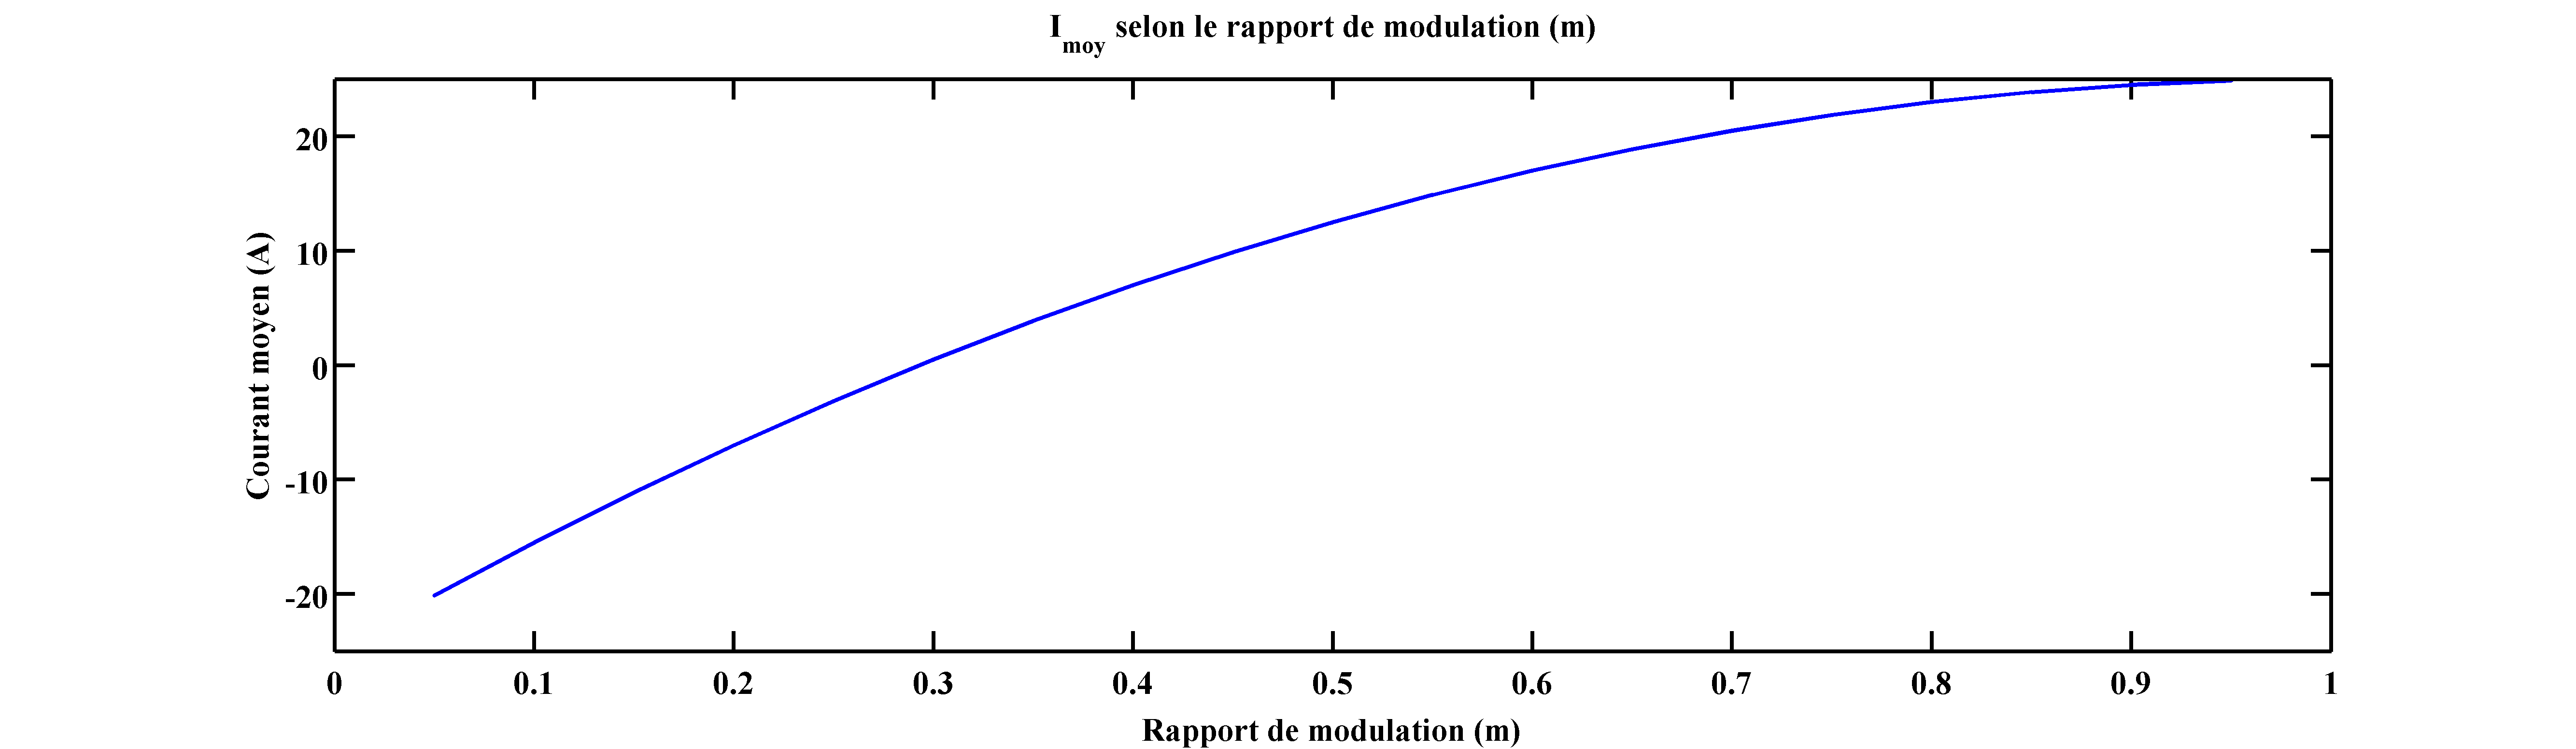
\includegraphics[scale=0.4]{fig/Imoy_m.png}
\caption{Courant moyen en fonction du rapport de modulation dans un onduleur monophasé}
\end{figure}

\section{Fonctionnement d'un onduleur monophasé NPC à 3 niveaux}
Le schéma d'un onduleur monophasé NPC à 3 niveaux est présenté à la figure \ref{eq1}. Un onduleur monophasé NPC à 3 niveaux est composé de 4 transistors, de 6 diodes et de deux condensateurs rattachés au point neutre (point central sur la figure \ref{eq1}). La configuration présentée a pour objectif d'obtenir des niveaux distincts de tension $V_{DC}$ à appliquer aux bornes des électroaimants. Dans cette configuration, chaque transistor ne commute pas toute la tension $V_{DC}$, l'avantage étant qu'on peut utiliser des composantes dont le dimensionnement est moins imposant que celles nécessaire pour fournir une puissance équivalente dans un montage à 2 niveaux classique. 

\paragraph{}Il existe 4 transistors IGBT qui commutent par paires. Les séquences possibles et les tensions produites sont décrites dans le tableau suivant:

\begin{table}[htb]
\centering
\begin{tabular}{ |c|c|c| }
\hline
  Type de séquence & Transistors activés & Niveau de tension \\\hline\hline
  P & [1,2] & $+V_{DC}$ \\\hline
  N & [3,4] & $-V_{DC}$ \\\hline
  O & [1,3] & $0$ \\\hline
  O & [1,4] & $0$ \\\hline
  O & [2,4] & $0$ \\\hline
\end{tabular}
\end{table}

En excluant les états redondants, il existe 3 états distincts, soit l'état P ([1,2]), l'état N([3,4] et l'état 0([1,3]). Une stratégie de commande simple et applicable est celle d'une modulation MLI à plusieurs niveaux. On réfère ici à la figure \ref{fig_MLI_ML} pour une illustration graphique de la commande MLI multiniveaux. À chaque période de commutation, une comparaison entre l'onde désirée et le signal en dent de scie. Pendant la période où le signal est plus grand (en valeur absolue) que le signal en dent de scie, la paire de transistor associée est activée pendant la période de conduction calculée. 

\begin{figure}[htb]
\centering
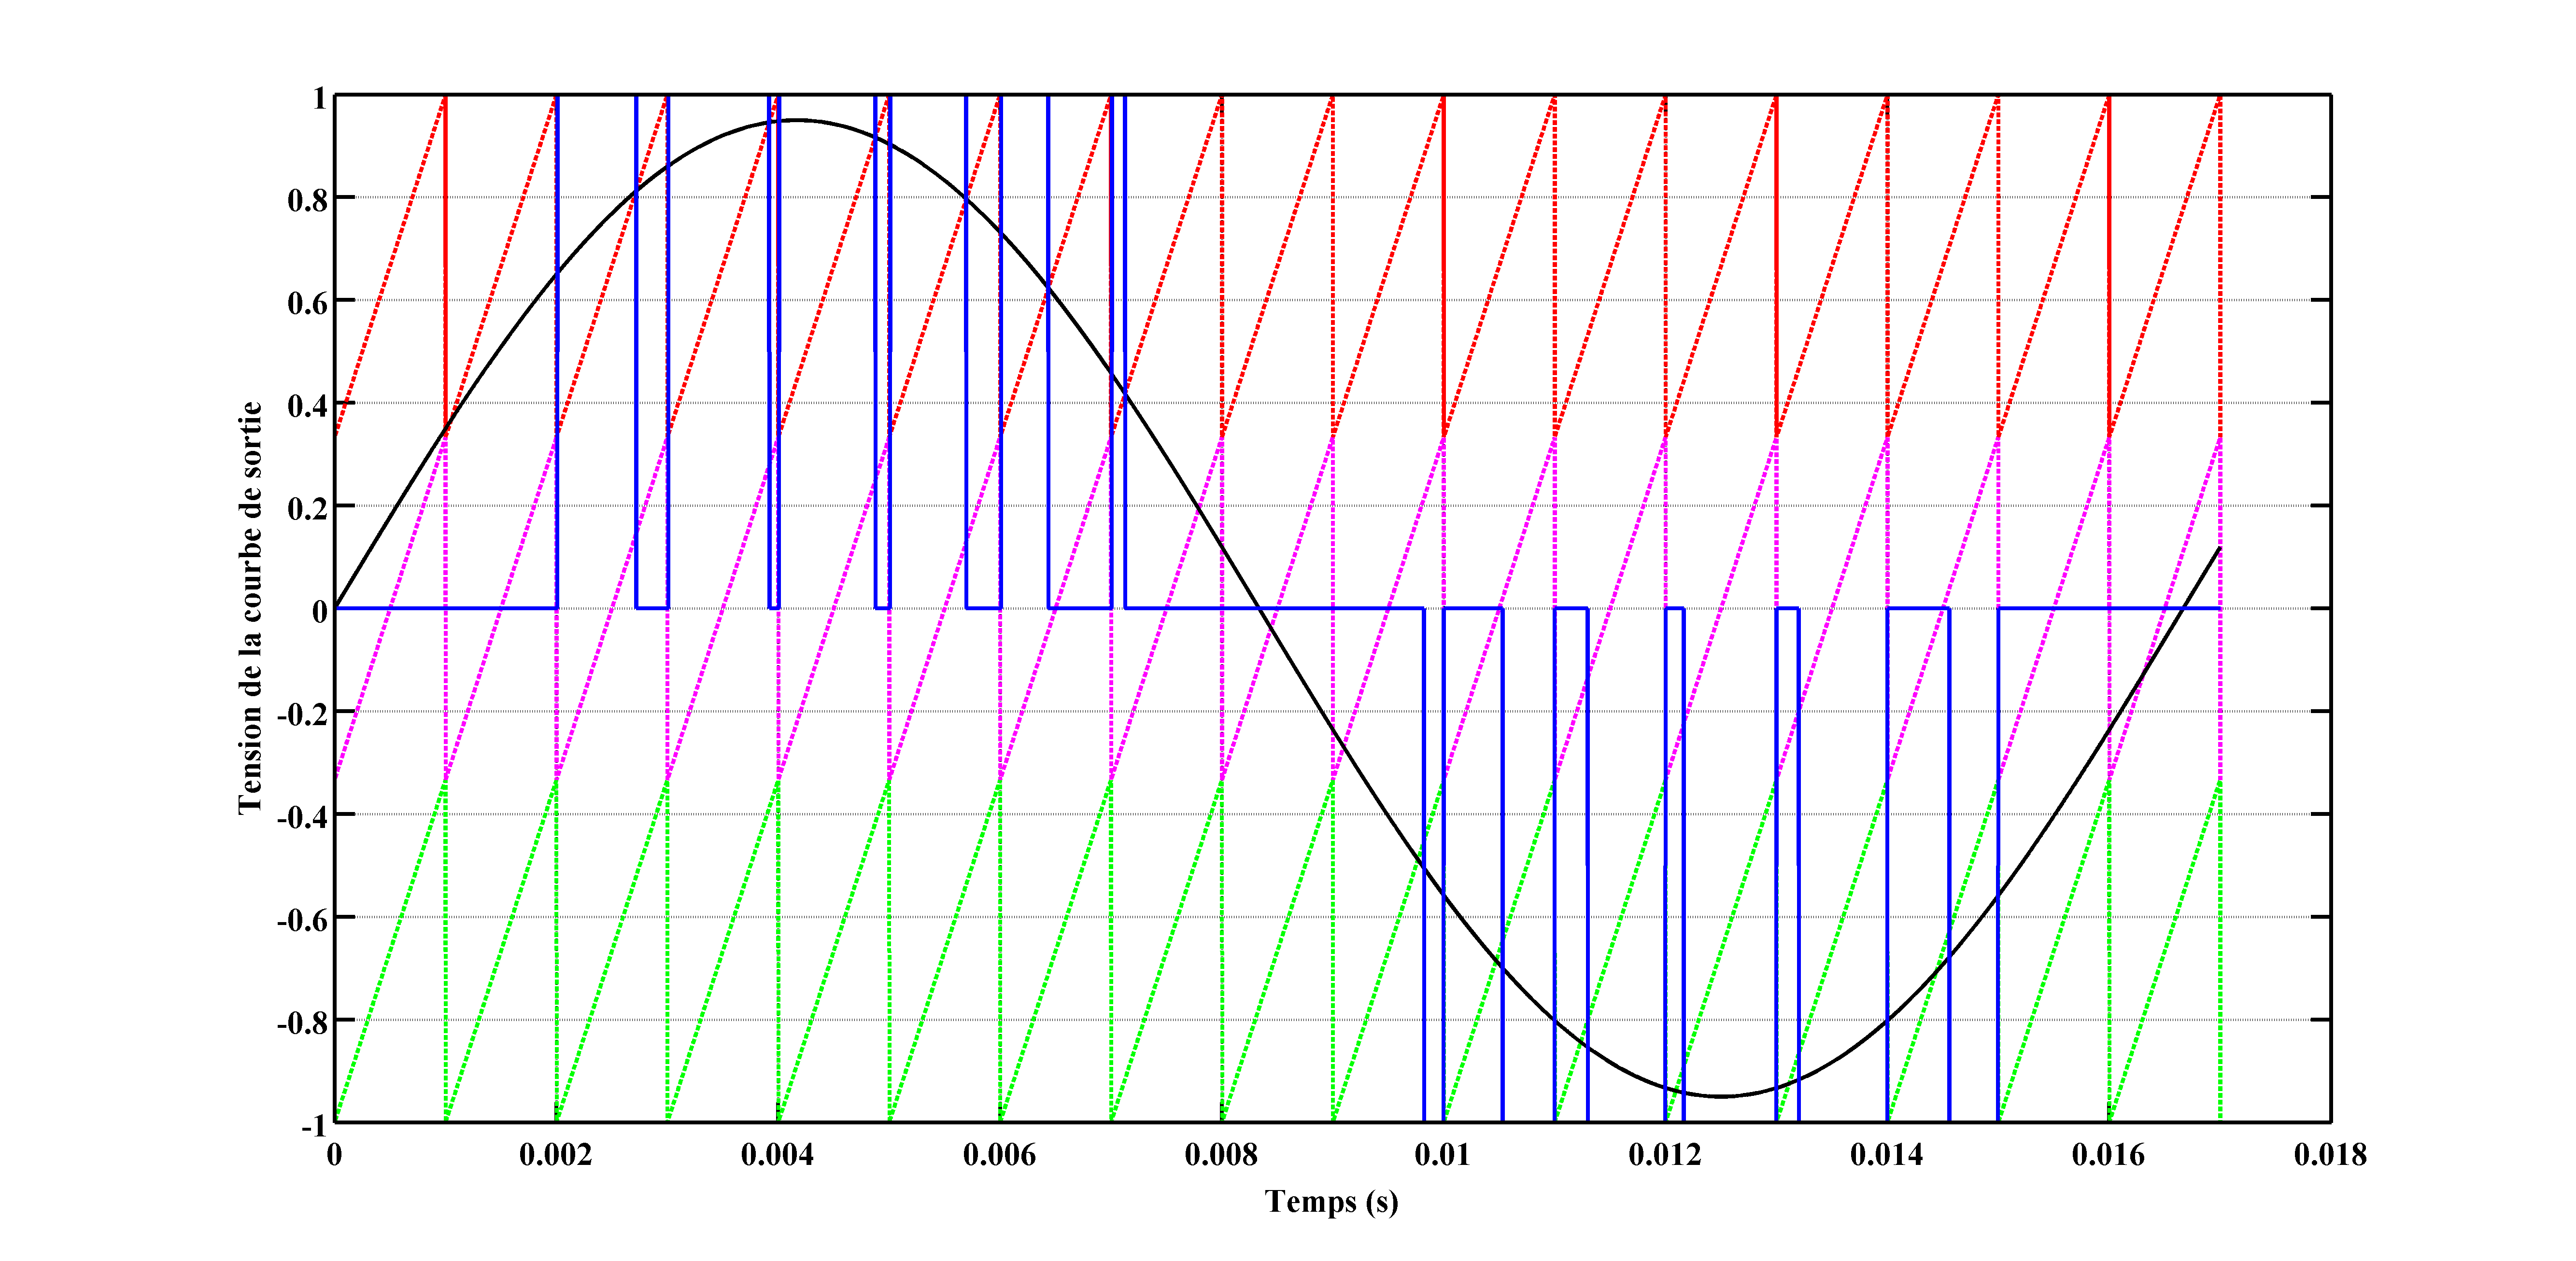
\includegraphics[scale=0.4]{fig/commande_NPC_1.png}
\caption{Commande MLI multiniveaux pour une consigne sinusoïdale}
\label{fig_MLI_ML}
\end{figure}

\section{Calculs théoriques liés à l'onduleur NPC 3 niveaux}
L'avantage d'une configuration NPC 3 niveaux est la diminution de la tension vue par chaque interrupteur. On considère premièrement que le bus d'alimentation est un bus CC parfait d'une tension de 5kV (selon les spécifications du projet) et qu'il n'y a pas de baisse de tension en fonctionnement normal. Chaque interrupteur est amorcé au tiers de la fréquence vue à la charge, soit à 330Hz, de plus comme l'onduleur proposé par le client utilise un décalage des phases d'un tiers de période, la conduction de chaque bras est donc limitée à 1ms sur 3ms. La tension vue sur l'interrupteur supérieur est limitée à 2.5kV, étant donné la présence d'un point milieu. L'utilisation de 2 cellules NPC 3 niveau permet d'appliquer $\pm$ 5kV aux bornes de la charge. Les interrupteurs doivent donc minimalement tenir une tension de 2.5kV. 

\paragraph{}L'entrelacement des bras et l'utilisation d'une tension suffisamment élevée sur le bus DC permet de limiter le temps de conduction des IGBT et donc, le courant moyen qui y est vu. Le courant maximal demandé par la charge est de 6000A. Afin de calculer le temps d'exposition maximal d'un interrupteur à ce courant, on utilise la tension minimale atteinte par le bus CC. Cette tension est de l'ordre de 3.25kV. Chaque interrupteur voit la moitié de cette tension. soit 1.625kV. La charge étant modélisée comme une inductance pure de 0.1H. En appliquant l'équation \ref{eq_Imoy}, on détermine que le rapport de modulation minimal est de 0.2929, afin de maintenir un courant moyen nul autour d'une consigne, en supposant qu'on ait un courant dans la charge dont la valeur moyenne ait atteint la consigne désirée. La valeur obtenue à partir de cette équation permet de fournir une première itération pour le calcul du courant $RMS$ circulant dans les interrupteurs. En supposant un rapport de modulation de 0.2929, pour une période de 3ms, avec un courant Imax de 6000A, on peut calculer le courant $RMS$ circulant dans l'interrupteur:
\begin{eqnarray}
I_{RMS} &=& \sqrt{\frac{1}{T}\int_0^{m_xT}I_{max}^2 dt}\\
I_{RMS} &=& \sqrt{333\int_0^{878\mu s}6000^2 dt}\\
I_{RMS} &=& 3244.2A RMS
\end{eqnarray}
Selon la commande appliquée, le $m_x$ peut changer étant donné qu'on ne fixe pas nécessairement un courant $I_{moy}$ à 0. Aussi, il est impératif de considérer les pertes qui peuvent faire fluctuer les résultats. Afin de calculer le courant moyen dans la charge, on suppose qu'une période est égale à 2.4s, tel que spécifié dans la documentation du CERN. Afin de simplifier les calculs, on suppose que chaque bras conduit $\frac{1}{3}$ du temps et donc que la période, vue d'un bras, est de 7.2s. Soit la forme de courant présentée à la figure \ref{fig_ref_courant}. Il est possible de calculer la valeur RMS du courant selon l'équation précédemment décrite précédemment. L'intégrale est réalisée au moyen de Matlab. On trouve que le courant RMS moyen d'un interrupteur d'un bras pour un cycle de 2.4s (7.2s vue de l'interrupteur), est de 1107A. 

\begin{figure}[htb]
\centering
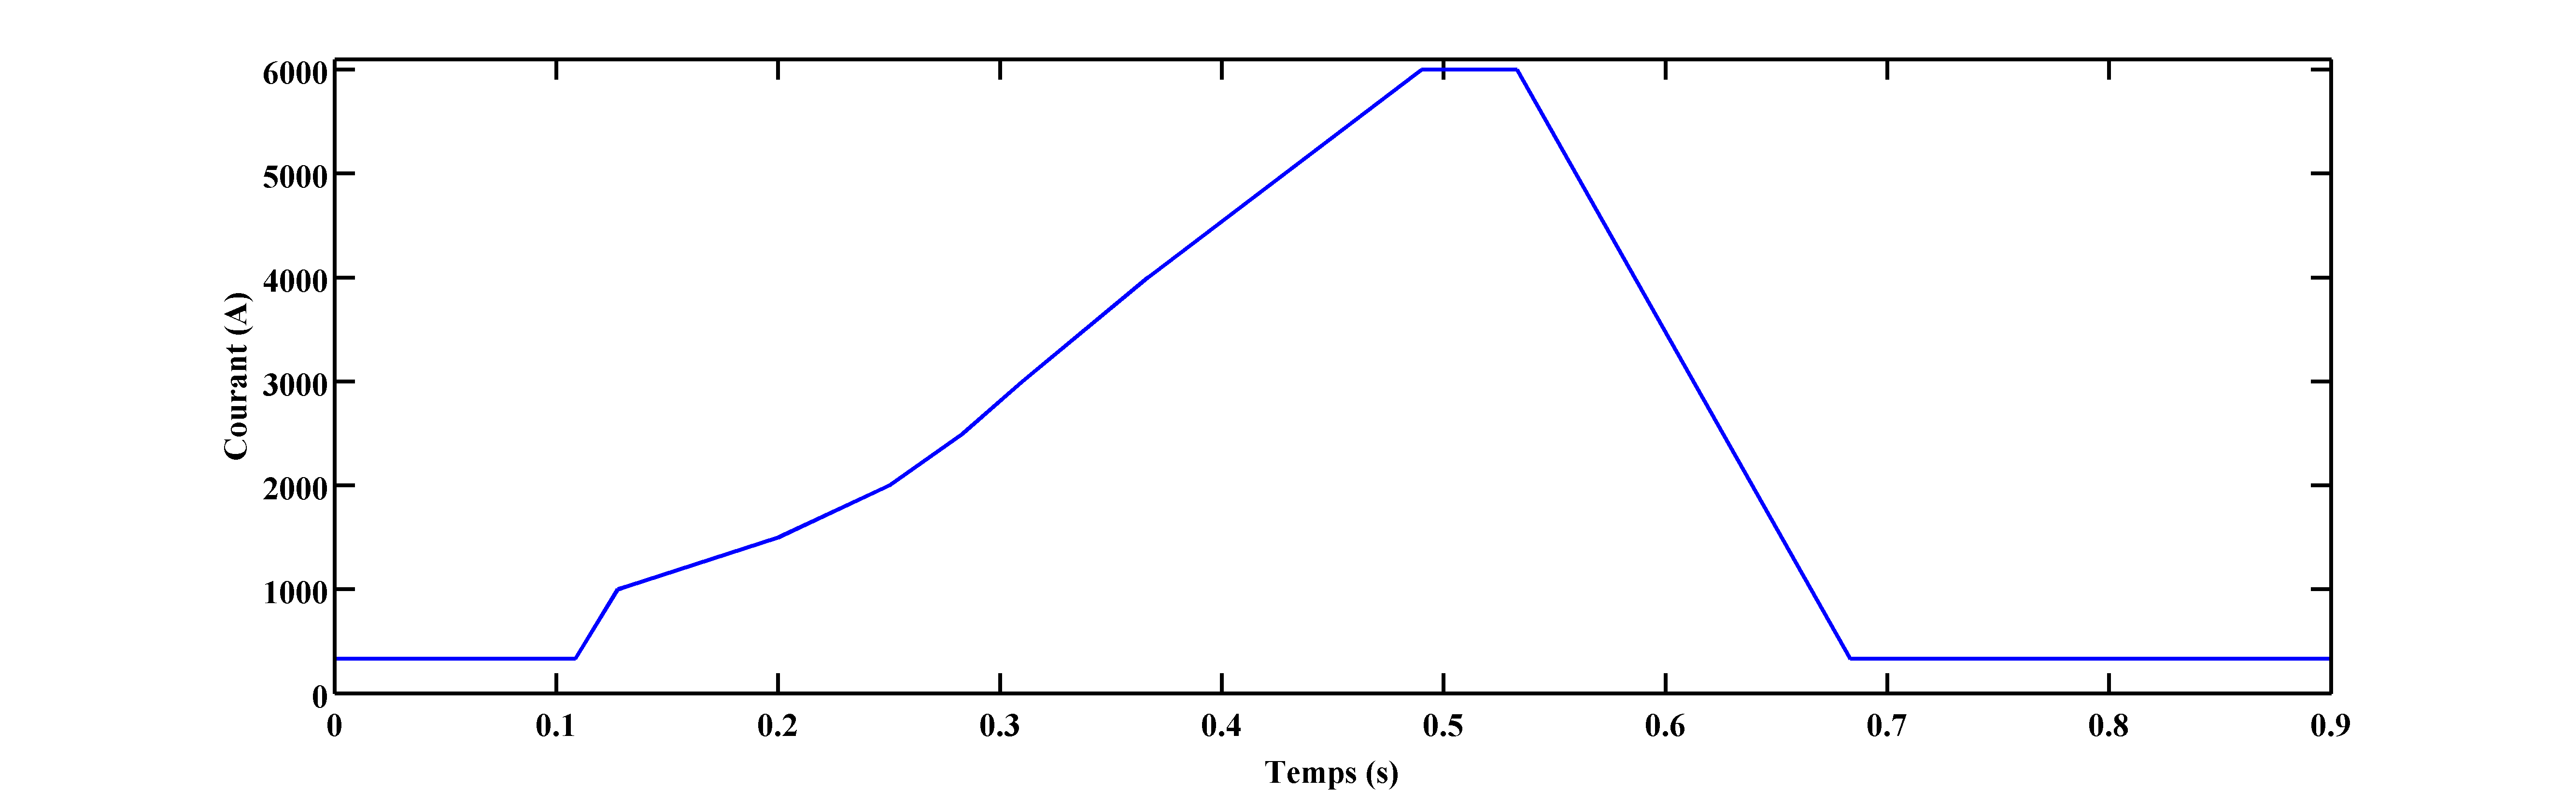
\includegraphics[scale=0.4]{fig/fig_ref_courant.png}
\caption{Référence de courant des électroaimants en A en fonction du temps (s)}
\label{fig_ref_courant}
\end{figure}

\section{Comparaison des résultats de dimensionnement théoriques obtenus par rapport à ceux du CERN}
Les résultats théoriques et ceux fournis par le CERN sont présentés au tableau \ref{tab_comp_1}. On remarque qu'il est possible d'obtenir un ordre de grandeur respectable des valeurs fournies par le CERN en effectuant des approximations théoriques et en utilisant une version échantillonnée à la main de la courbe de référence de courant. On comprend que les interrupteurs du CERN ne sont pas maintenus à un courant moyen de 0, tel qu'il était prévu, ils sont maintenu à un rapport cyclique (sur 3ms) de 0.25. Ne disposant pas précisément des méhodes de commandes et des formes d'ondes vues à la charge, il est difficile d'obtenir une approximation plus précise. Cependant, on remarque que les interrupteurs sont dimensionnés pour les valeurs RMS maximales vue sur la crête de 6kA et que la valeur moyenne (RMS) des interrupteurs est calculée sur un cycle de 2.4s. L'écart étant faible entre les données calculées théoriquement et celles du CERN, on suppose qu'à cet effet ils utilisent un rapport cyclique de 1/3, soit 1ms/3ms, par interrupteur. La valeur moyenne de tension tient compte que la tension du bus CC peut monter à 5100V. Aussi, si l'on se réfère aux spécifications techniques des interrupteurs employés pour les tests, on remarque que la tension qu'ils tiennent est de l'ordre de 4.5kV. Le courant maximal moyen en valeur RMS varie de 1460 A à 1780 A, selon le type d'interrupteur. La valeur crête du courant RMS respecte les valeurs $I_{MaxComm}$ qui vont de 4000 A à 5500 A.

\begin{table}[htb]
\centering
\begin{tabular}{ |c|c|c| }
\hline
  Paramètre & Théorie & CERN\\\hline\hline
  $I_{FAVRMS}$ (A) & 1107 A & 1070 A \\\hline
  $I_{PeakRMS}$ & 3244 A & 3000 A \\\hline
  $I_{Peak}$ & 6 kA & 6 kA \\\hline
  $V_{AV}$ & 2.5 kV & 2.75 kV \\\hline
\end{tabular}
\caption{Comparatif des résultats théoriques et de ceux fournis par le CERN}
\label{tab_comp_1}
\end{table}
\chapter{Validation croisée entre les simulateurs}
Ce chapitre présente une comparaison des simulateurs selon les paramètres des simulation critiques: courant dans les électroaimants, tension aux bornes des électroaimants, courant à l'entrée de l'AFE, tension du bus CC, courants et tensions dans les IGBT. Les sous-modèles se séparent en plusieurs catégories, soit les simulations représentant l'AFE, ceux représentant le convertisseur CC-CC et ceux représentant un montage avec un AFE et un convertisseur CC-CC. Il est à noté que le temps de simulation qui est employé pour fins d'analyse est de 1$\mu$s. 

\section{Comparaison entre PSIM et SPS}
Cette section décrit des comparaisons faites sur le fonctionnement des éléments de bases fondamentaux pour le projet, dans les simulateurs PSIM et SPS.
\subsection{Algorithmes de simulation sur PSIM et SPS}
PSIM et SPS utilisent des méthodes de résolution différentes. SPS est un outil de simulation puissant et générique. Il établit un système d'équations d'états à partir du modèle de simulation, ces équations permettant de déterminer la solution du circuit. Les éléments non-linéaires sont modélisés comme des sources de courants. Les interrupteurs sont modélisés par une faible résistance en conduction et une forte résistance en blocage. Afin d'obtenir des modèles discrets, SPS discrétise les équations d'états continues en utilisant la méthode de Tustin  \footnote{http://www.mathworks.com/products/simpower/description4.html, 17 avril 2014}, la figure \ref{fig_solving_SPS} présente un résumé schématique de l'implémentation. Afin d'augmenter la vitesse de simulation de l'électronique de puissance, SPS utilise un algorithme dans lequel les commutations sont idéales. Il existe deux méthodes de détection des passages par zéro dans SPS , soit la méthode Tustin  (équivalente à une méthode trapézoïdale) et la méthode Backward Euler. La méthode trapézoïdale offre une meilleur précision pour un temps de calcul fixe, mais peut parfois présenter des oscillations numériques. La méthode Backward Euler est moins précise pour un pas de simulation donné, mais permet d'éviter les oscillations numériques. PSIM implémente les modèles au moyen d'une matrice d'admittance nodale\footnote{http://powersimtech.com/support/frequently-asked-questions/, 17 avril 2014}. Les interrupteurs sont idéaux et représentés par une résistance faible en conduction et par une résistance élevée en blocage. La méthode de simulation de PSIM est moins adaptée à l'étude des transitoires pour l'électronique. Elle est cependant plus rapide et permet des études de plus haut niveau. La méthode de détection des passages par zéro de PSIM est une méthode trapézoïdale. 

\begin{figure}
\centering
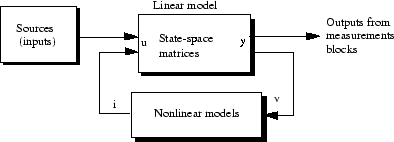
\includegraphics[scale=0.7]{Fig/Comp/improving_performance5.png}
\caption{Méthode de solution des systèmes implantée dans SPS}
\label{fig_solving_SPS}
\end{figure}

\subsection{Comparaison des modèles d'IGBT}

\begin{figure}[htb]
\centering
\includegraphics[scale=0.5]{fig/Comp/IGBT.jpg}
\caption{Commutation d'un IGBT à un pas de calcul de 5$\mu$s}.
\label{IG}
\end{figure}

Les IGBT sont les interrupteurs utilisés dans chacun des sous-modèles simulés du projet. On remarque sur la figure \ref{IG} que le  courant traversant l'IGBT est identique dans le cas d'un IGBT sur une charge résistive de 50k$\Omega$. Le pas de calcul employé sur les deux plateformes est de 5$\mu$s. L'indice de modulation des IGBT est de 0.5 et la fréquence de commutation de 1 kKHz. Le montage est alimenté par une tension continue de 1kV et possède une résistance interne de 0.01$\Omega$. 

Sur SPS, l'IGBT possède un snubber RC intégré, tandis que sur PSIM il faut l'incorporer manuellement. Pour les deux simulations, le snubber employé est une résistance de 100k$\Omega$.
 
\subsection{Contrôleur proportionnel-intégrateur (PI)}
L'implantation des blocs PI est différente entre SPS et PSIM. Sur SPS, il est possible d'obtenir une forme idéale ainsi qu'une forme parallèle, tandis que sur PSIM, les blocs par défaut ne comportent que la forme idéale. La forme parallèle doit être implantée manuellement. On remarque sur la figure \ref{PI} que les résultats sont identiques entre une implantation manuelle sur PSIM et le bloc par défaut de SPS. La valeur du gain intégrateur du PI est de 50 et celle du gain proportionnel de 0.071. 

\begin{figure}[htb]
\centering
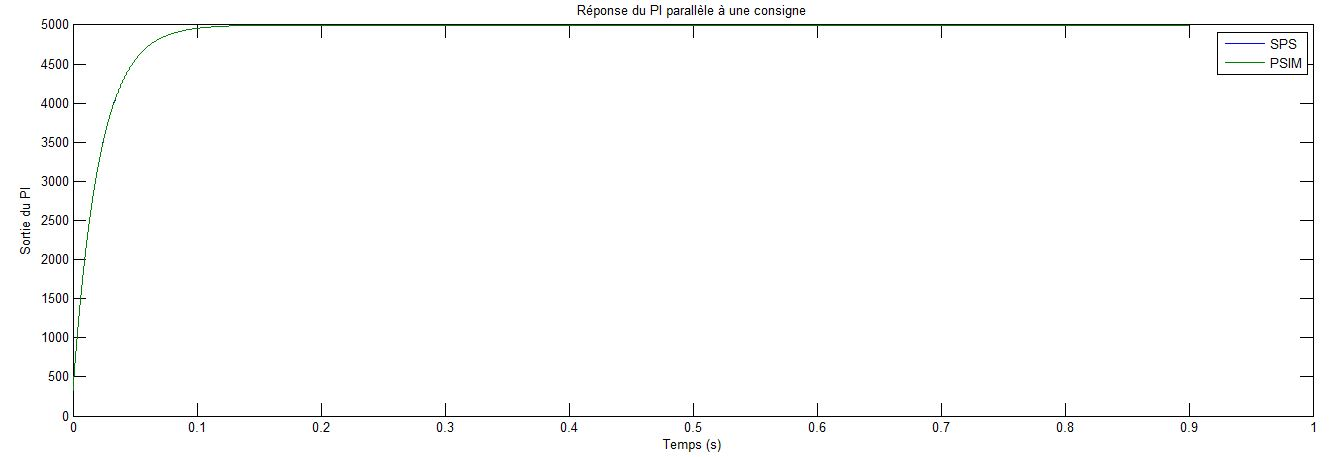
\includegraphics[scale=0.5]{fig/Comp/PI.jpg}
\caption{Réponse d'un contrôleur PI suite à une consigne d'erreur}.
\label{PI}
\end{figure}

\clearpage
\subsection{Calibration des contrôleurs (PI)}
Les contrôleurs PI sont calibrés en utilisant des modèles continus équivalents des charges alimentées par les convertisseurs et ce, en excluant l'impact de la modulation. L'objectif étant d'obtenir la constante de temps dominante du circuit. Soit un circuit RL série, qui représente les électroaimants à alimenter, il est possible d'établir que la constante de temps dominante du contrôleur PI du convertisseur est de $T_i = \tau = L/R$. Le modèle de base d'un contrôleur PI pouvant être représenté par une équation dans le domaine de Laplace de la forme: $H(s) = \frac{1 + K_p T_is}{T_i s}$. Il suffit par la suite de procéder à une analyse dynamique du comportement du convertisseur afin de déterminer le gain $K_p$ fournissant la réponse optimale. Par la suite, il est nécessaire de procéder à une discrétisation du régulateur selon le pas de calcul, selon la méthode de Tustin. 
\section{Convertisseur CC-CC 4 quadrants à 4 interrupteurs IGBT}
Le hacheur 4 quadrants, à proprement parlé, est constitué de 4 interrupteurs IGBT commandés au moyen d'une régulation MLI. La figure \ref{i_hach} présente le circuit électrique associé à un tel convertisseur. Ce type de montage est un montage de base utilisé afin de valider le concept de fonctionnement d'un convertisseur CC-CC et d'établir la méthodologie de comparaison des simulations. Le tableau \ref{p_hash} présente les paramètres utilisés pour le hacheur 4 quadrants.

\begin{figure}[htb]
\centering
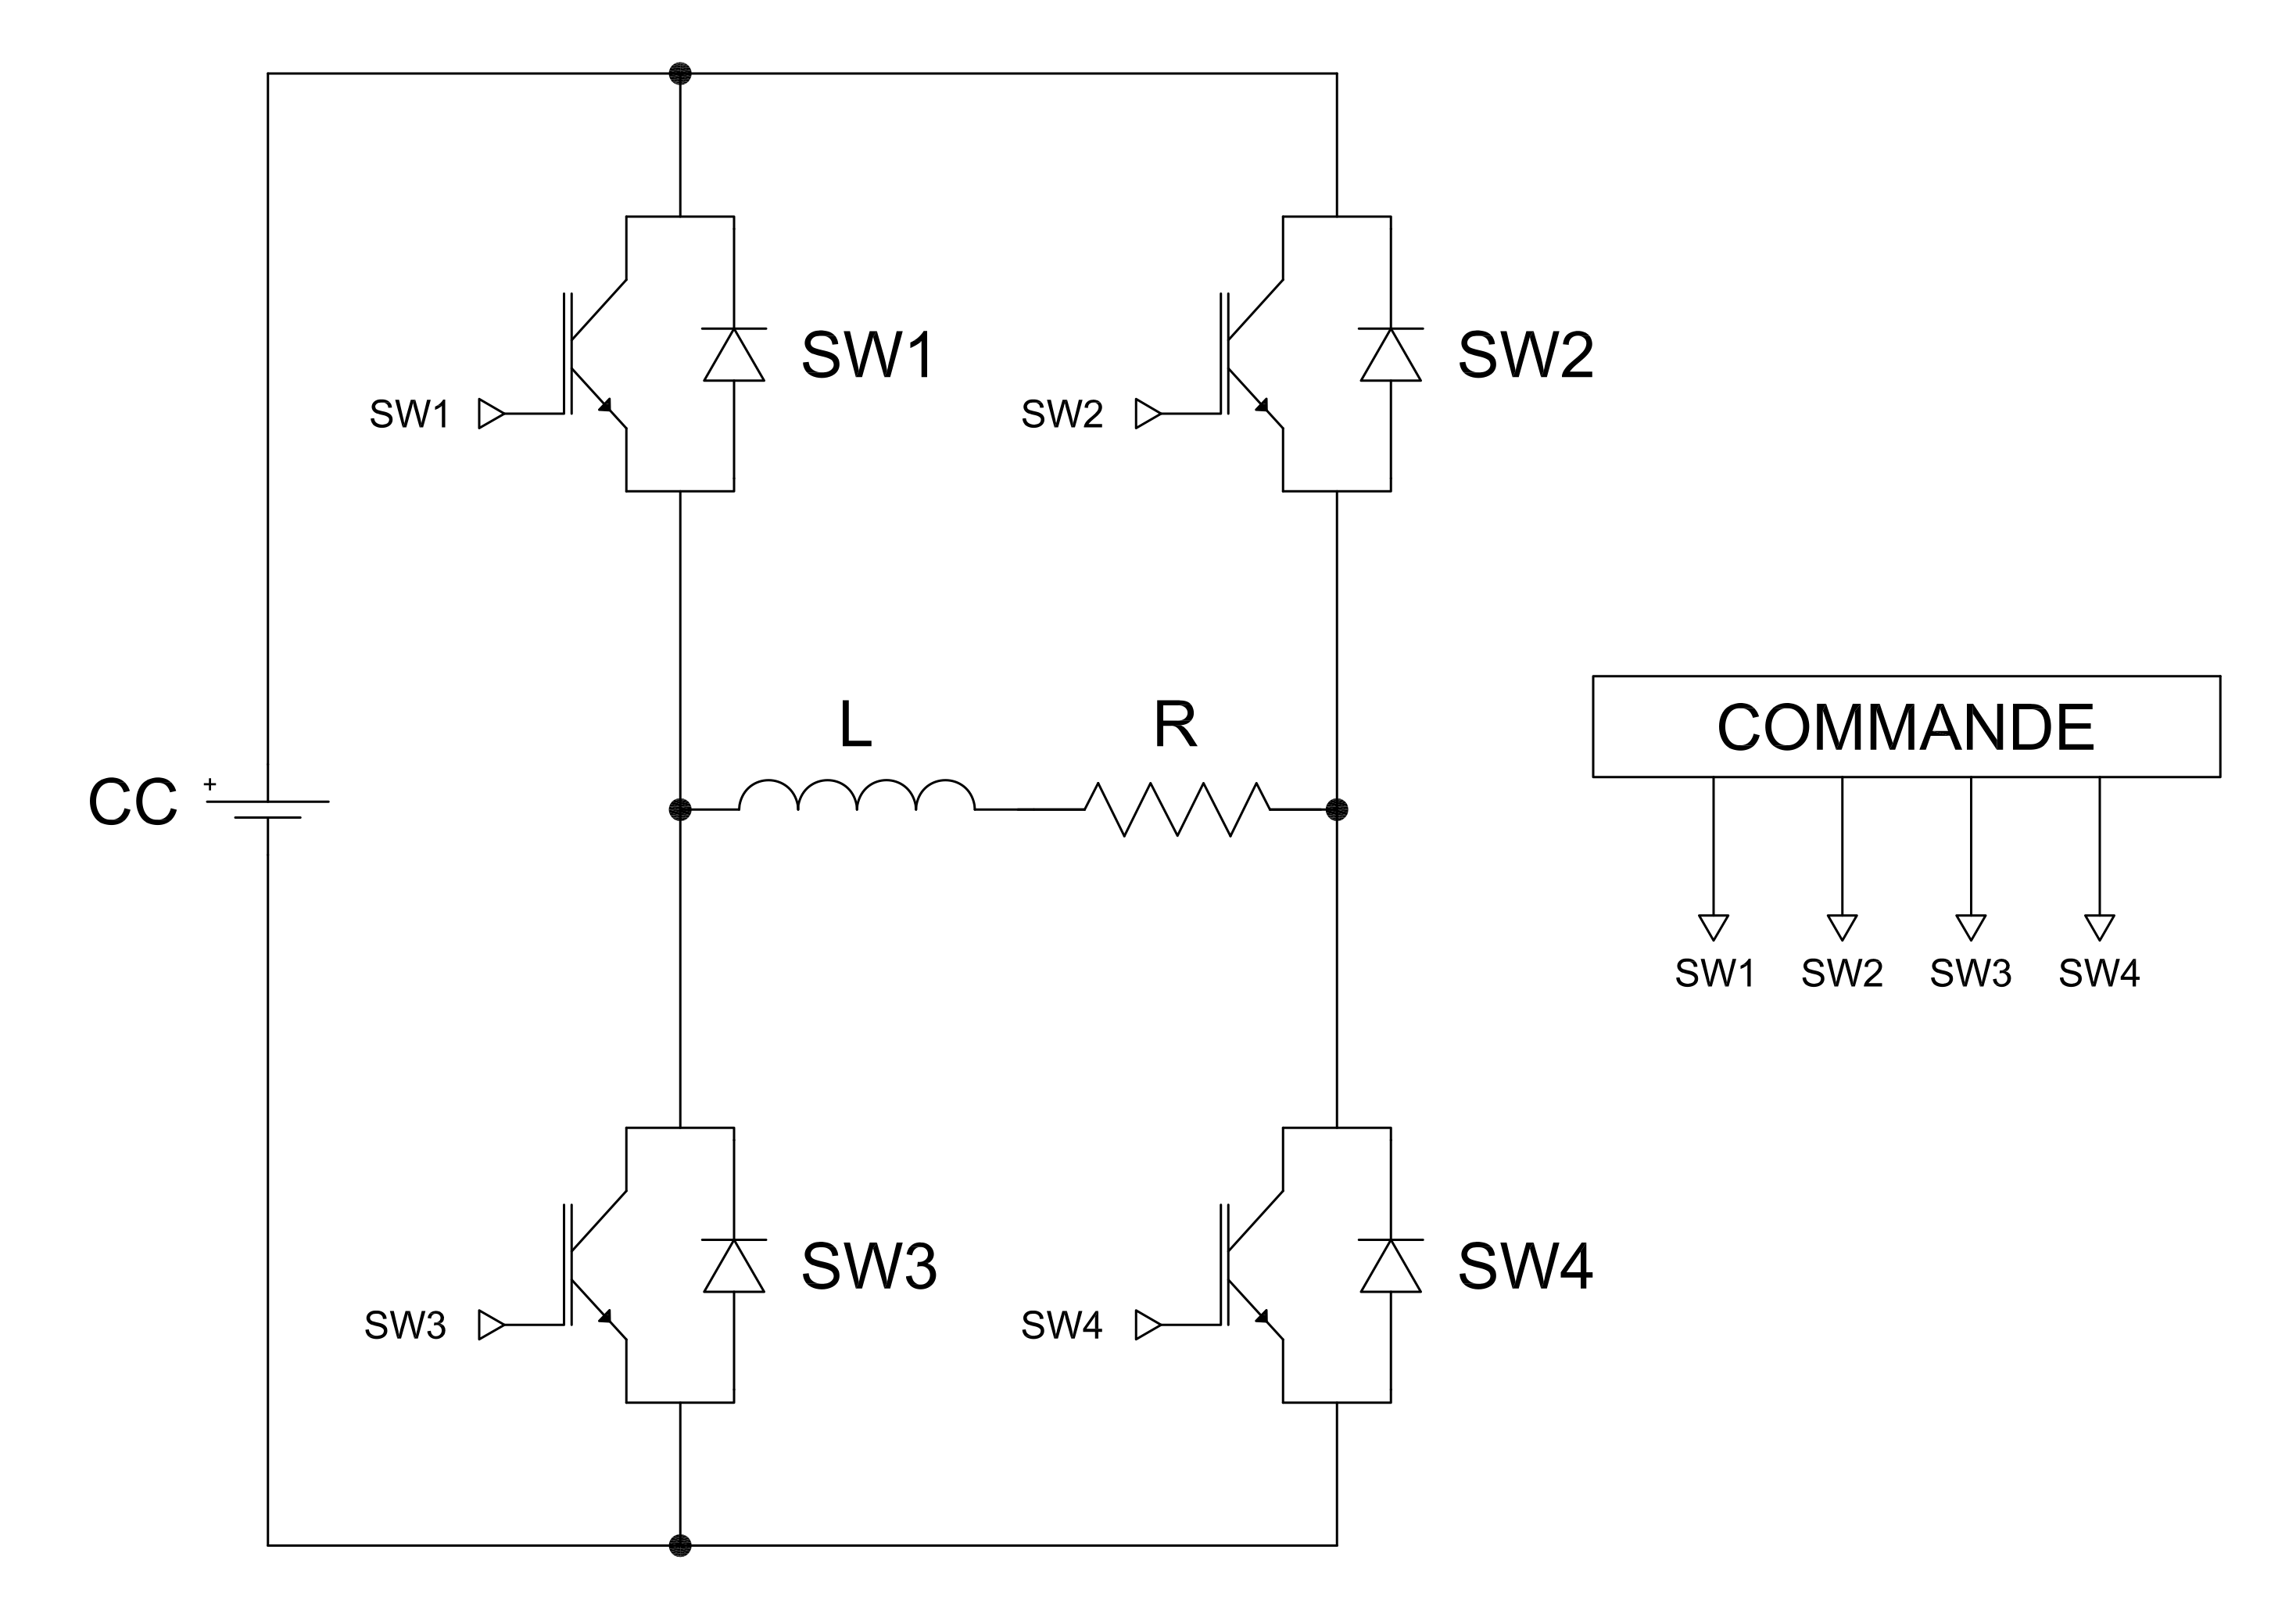
\includegraphics[scale=0.5]{fig/H4Q.png}
\caption{Circuit électrique du convertisseur CC-CC 4 quadrants à 4 interrupteurs IGBT}.
\label{i_hach}
\end{figure}

\begin{table}[htb]
\centering
\begin{tabular}{|l|c|} 
  \hline
  \textbf{Paramètre} & \textbf{Valeur}  \\
  \hline\hline
  Tension CC & 5000 V\\ \hline
  Fréquence de modulation & 1000 Hz\\ \hline
  Rapport cyclique maximal & 0.95 \\ \hline \hline
  \multicolumn{2}{|l|}{\textbf{IGBT}}\\ \hline
  Résistance interne & 0.001 $\Omega$\\
  Résistance du snubber & 100k $\Omega$\\ \hline \hline
   \multicolumn{2}{|l|}{\textbf{PI}}\\ \hline
  Gain proportionnel & 0.071 \\
  Gain intégrateur & 50 \\ \hline \hline
  \multicolumn{2}{|l|}{\textbf{Charge}}\\ \hline
  Résistance & 0.28 $\Omega$\\
  Inductance & 0.1 H\\
  \hline
\end{tabular}
\caption{Paramètres de simulation pour le convertisseur CC-CC à 4 interrupteurs}
\label{p_hash}
\end{table}

\subsection{Résultats de simulation pour SPS et PSIM pour un pas de calcul de 1$\mu$s}
Cette section présente les résultats de simulations du convertisseur CC-CC 4 quadrants, formé avec 4 interrupteurs IGBT, pour un pas de calcul de 1$\mu$s. 


\begin{figure}[htb]
\centering
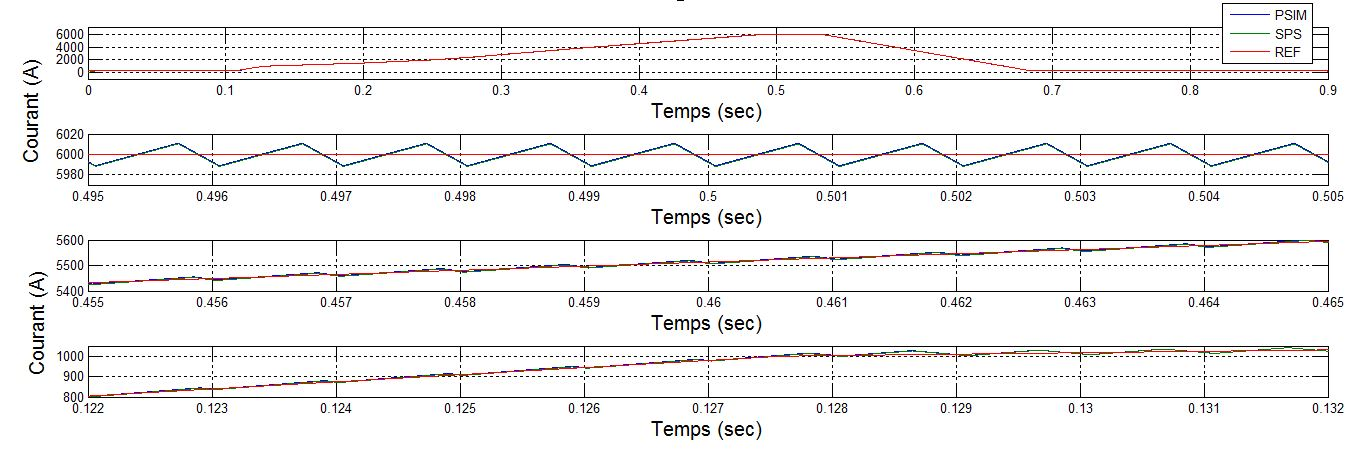
\includegraphics[scale=0.5]{fig/Hacheur4Quadrants/HacheurCourantCharge1u.jpg}
\caption{Courant traversant la charge sur PSIM et SPS pour un pas de calcul de 1$\mu$s, pour le hacheur 4 quadrants}
\label{hc_cou_ch_1}
\end{figure}


\begin{figure}[htb]
\centering
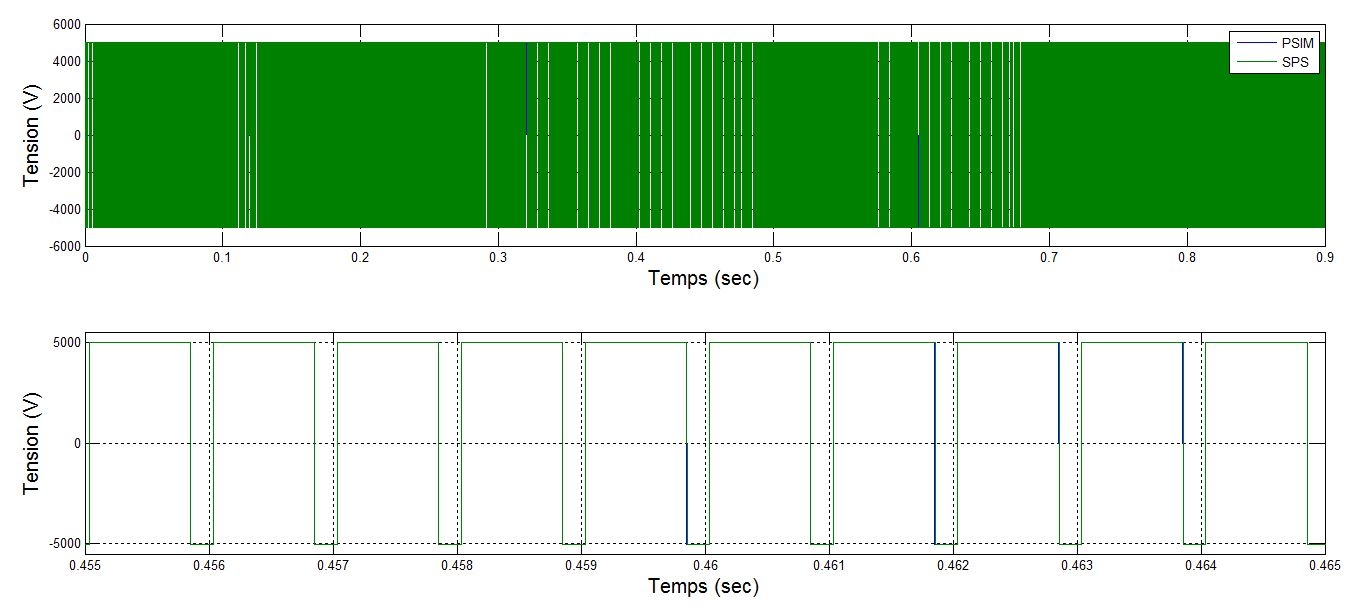
\includegraphics[scale=0.5]{fig/Hacheur4Quadrants/HacheurTensionCharge1u.jpg}
\caption{Tension aux bornes de la charge sur PSIM et SPS pour un pas de calcul de 1$\mu$s, pour le hacheur 4 quadrants}
\label{hc_ten_ch_1}
\end{figure}


\begin{figure}[htb]
\centering
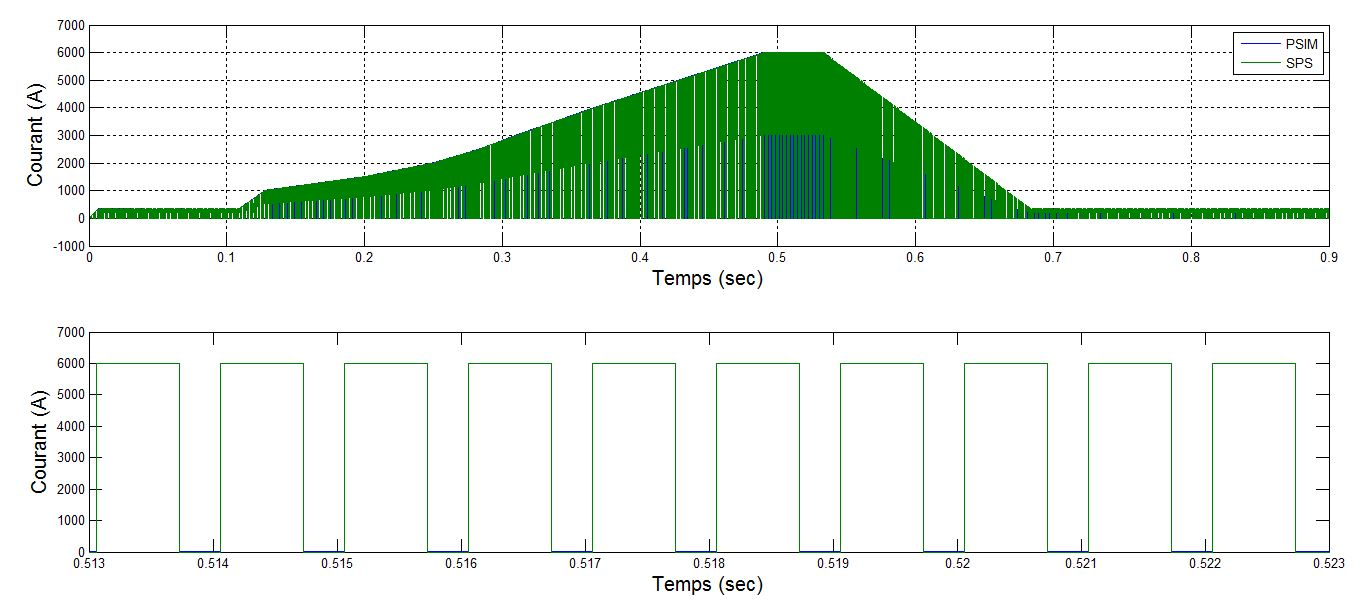
\includegraphics[scale=0.5]{fig/Hacheur4Quadrants/HacheurCourantIGBT1u.jpg}
\caption{Courant traversant un IGBT sur PSIM et SPS pour un pas de calcul de 1$\mu$s, pour le hacheur 4 quadrants}
\label{hc_IG_cou_1}
\end{figure}

\begin{figure}[htb]
\centering
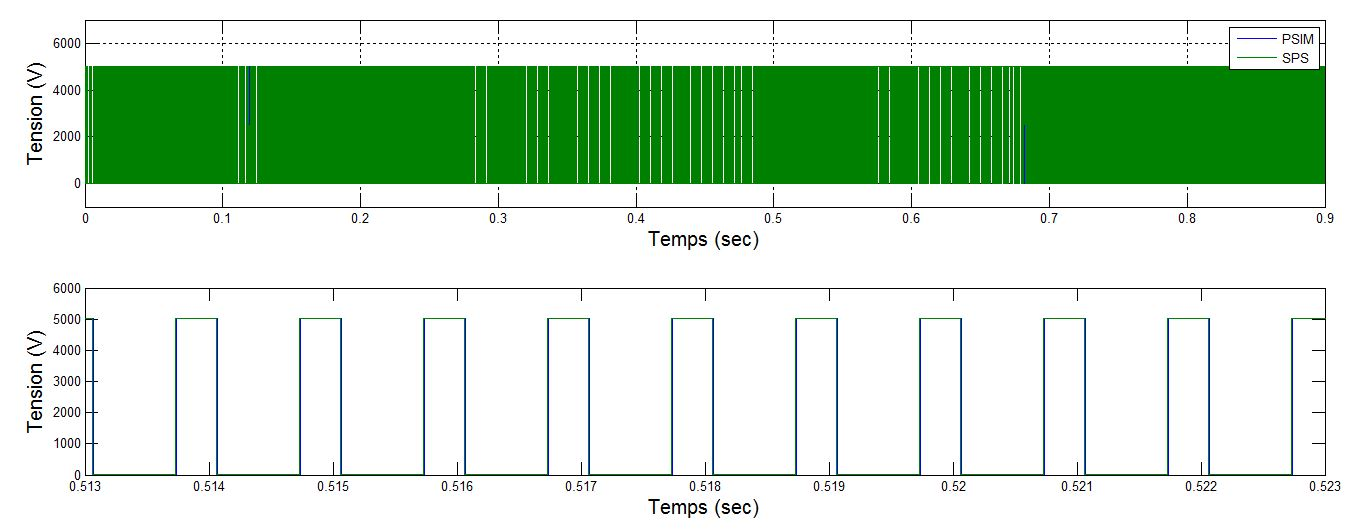
\includegraphics[scale=0.5]{fig/Hacheur4Quadrants/HacheurTensionIGBT1u.jpg}
\caption{Tension aux bornes d'un IGBT sur PSIM et SPS pour un pas de calcul de 1$\mu$s, pour le hacheur 4 quadrants}
\label{hc_IG_ten_1}
\end{figure}


\clearpage
\subsection{Analyse des résultats comparatifs de SPS et de PSIM pour un pas de calcul de 1$\mu$s}

Les résultats obtenus pour la simulation du hacheur 4 quadrants permettent d'établir la méthodologie du projet. On note que les simulations confirment le fonctionnement dans la zone de maintien du courant à 6kA, ce qu'on peut remarquer à la figure \ref{hc_cou_ch_1}. Il est pratiquement impossible de discerner des différentes dans les résultats de simulation pour ce cas. À la même figure, il est possible de noter les courants dans les différentes phases du cycle des électroaimants. On remarque que les courbes de PSIM et SPS sont presque parfaitement supersposée en montée. La figure \ref{hc_ten_ch_1} permet d'observer la tension aux bornes de la charge. On remarque qu'il est presque impossible de discerner une différence à l'échelle de la commutation entre les simulations. La conclusion est identique pour les figures représentant la tension et le courant vus par l'un des IGBT. Cette simulation simple d'un convertisseur CC-CC permet d'assoir la méthodologie de conception et d'observer le comportement du convertisseur CC-CC escompté Les considérations de filtrage de l'onde ont été prises en compte et on remarque qu'il ne semble pas y avoir une quantité de réammorçages excessives. La bande passante observée correspond donc à celle désirée et le comportement est corrélé à travers 2 simulateurs




\section{Convertisseur CC-CC 4 quadrants formé de 2 convertisseurs 3 niveaux NPC}
Le montage implanté au CERN est un convertisseur CC-CC formé de 2 onduleurs triphasés 3 niveaux NPC. La cellule supérieure est dénotée par DCP et la cellule inférieure par DCN. L'assemblage des onduleurs est tel qu'il permet le fonctionnement dans les 4 quadrants. Cette version reproduit le fonctionnement du hacheur 4 quadrants de base avec un plus grand degré de liberté. Il est composé au total de 24 interrupteurs IGBT/DIODE commandé par MLI ainsi que de 12 diodes de point milieu. La figure \ref{circuit_DCP_DCN} présente le circuit électrique du convertisseur. Le tableau \ref{p_DCP} présente les données utilisées pour ce sous-système.


\begin{figure}[htb]
\centering
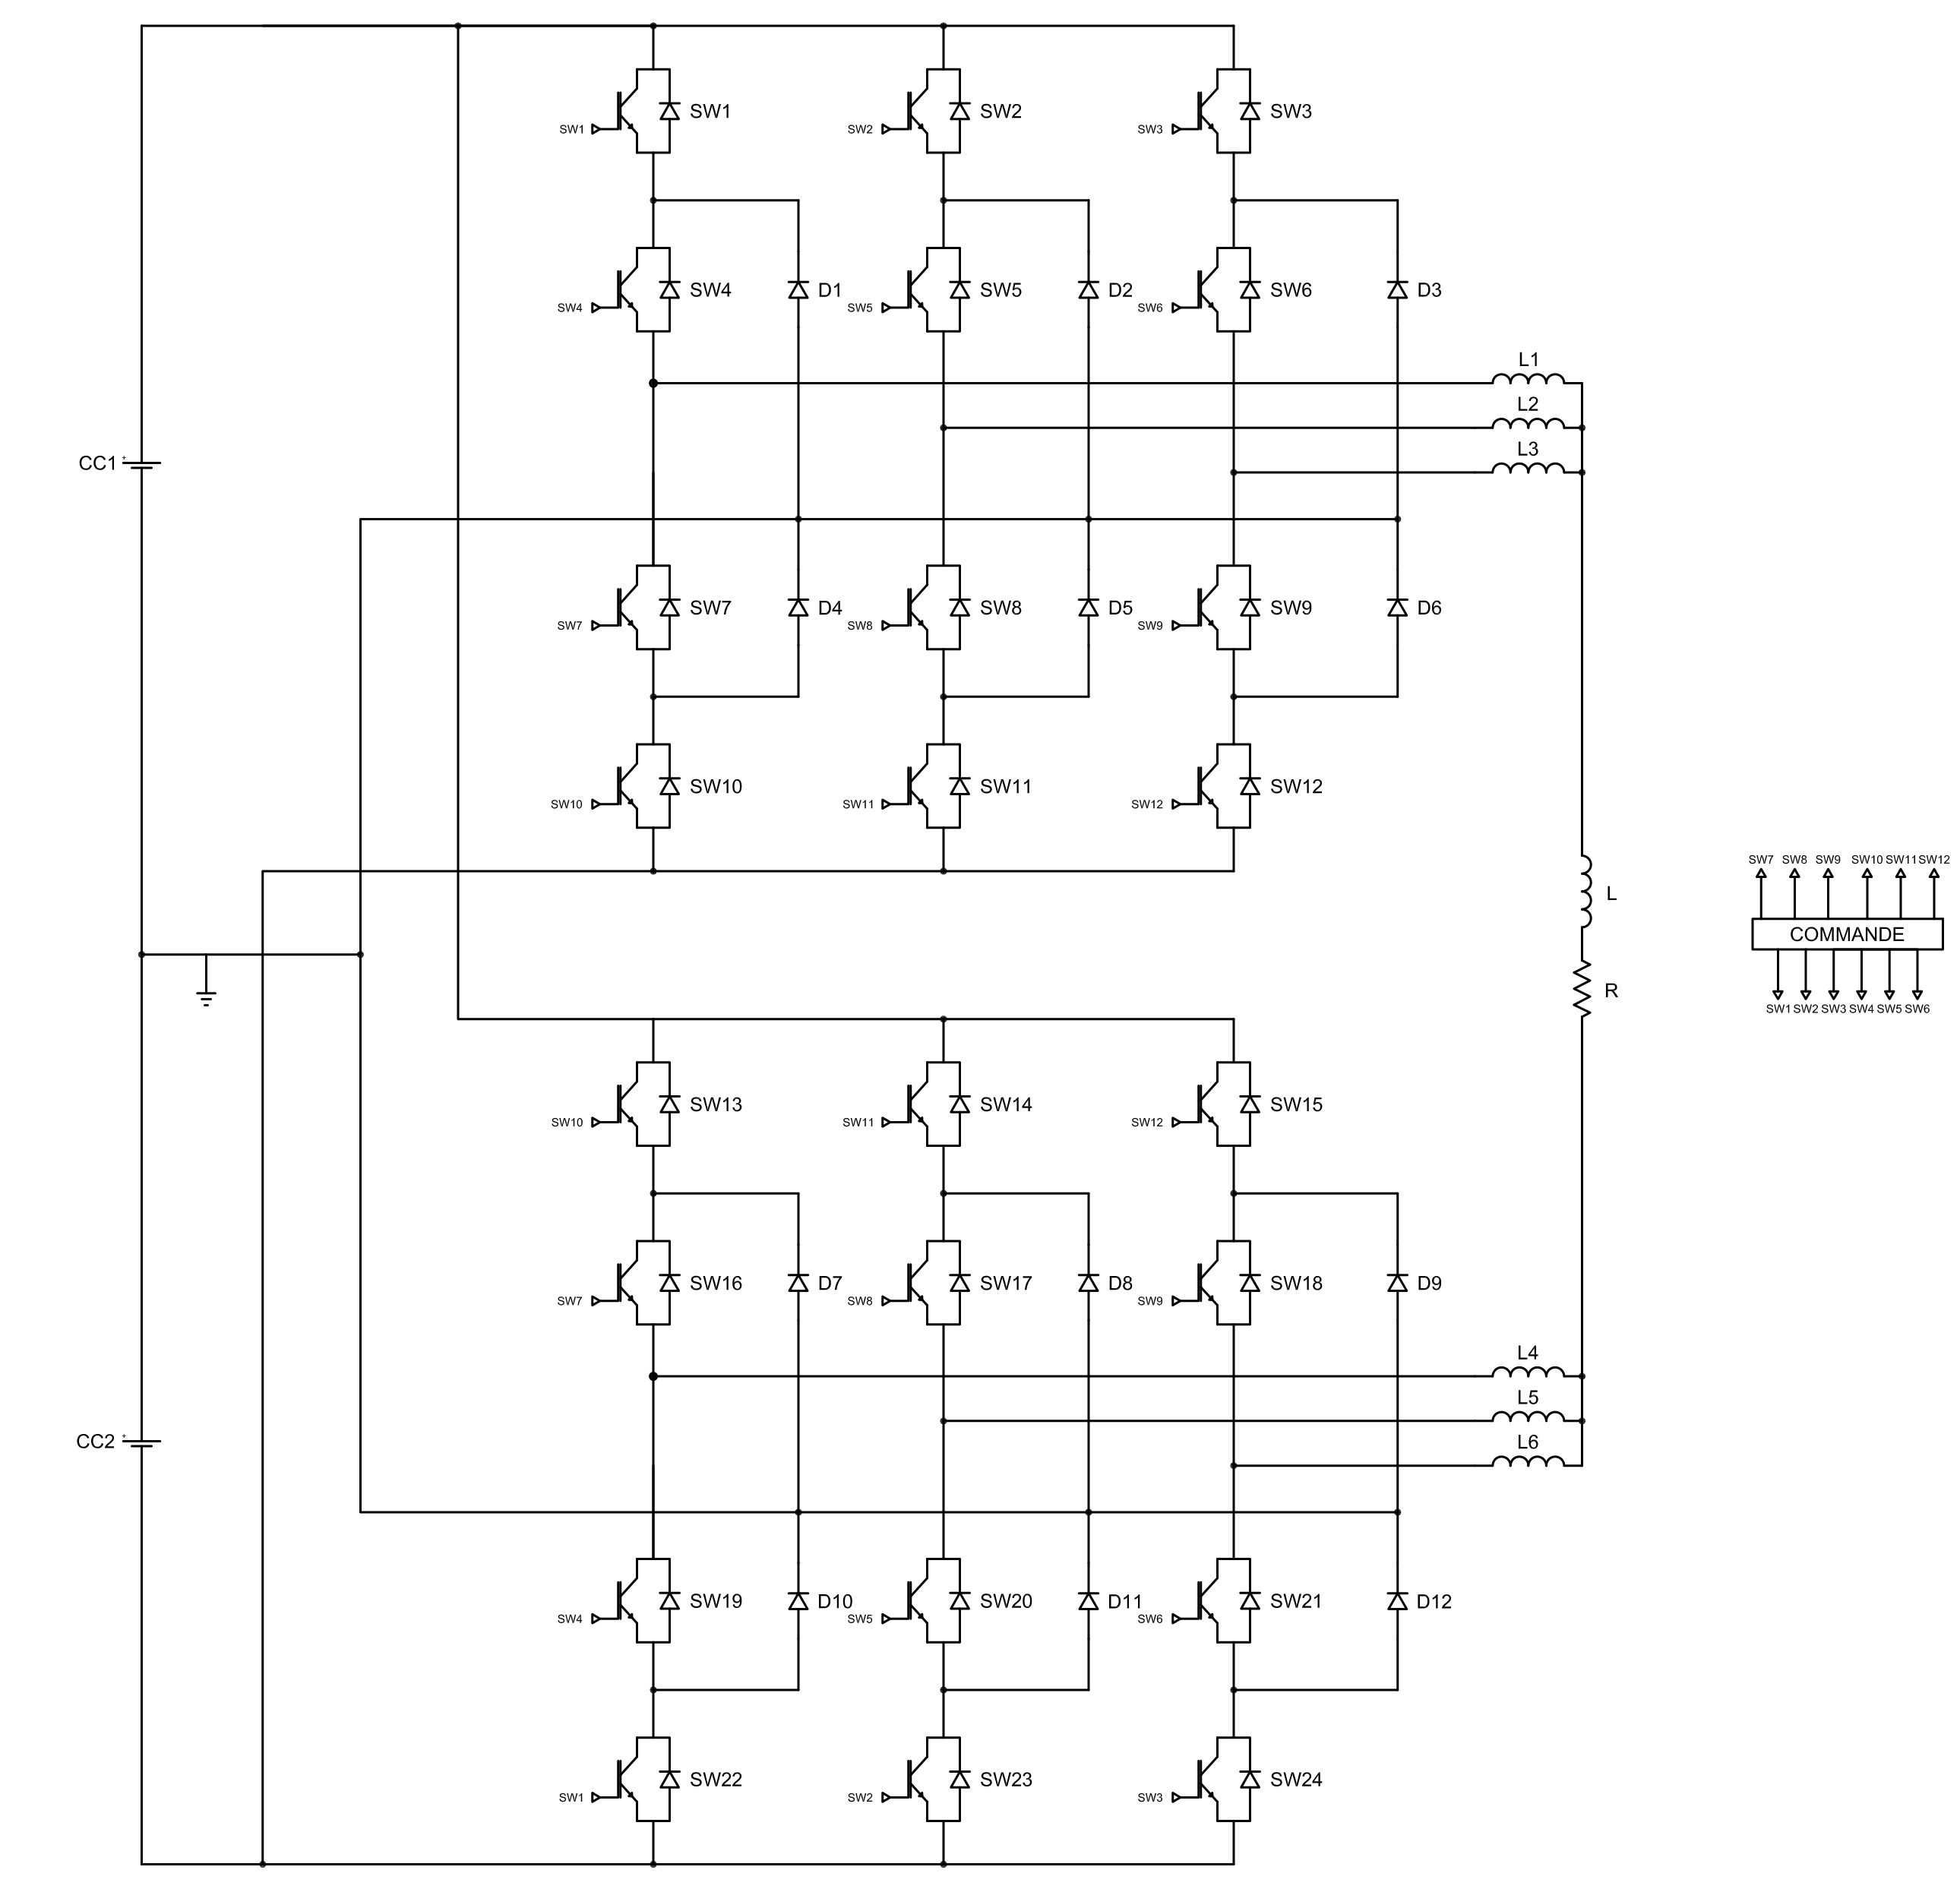
\includegraphics[scale=0.75]{fig/DCP_DCN.png}
\caption{Circuit électrique du convertisseur CC-CC 4 quadrants formé de 2 convertisseurs 3 niveaux NPC}
\label{circuit_DCP_DCN}
\end{figure}


\begin{table}[htb]
\centering
\begin{tabular}{|l|c|} 
  \hline
  \textbf{Paramètre} & \textbf{Valeur}  \\
  \hline\hline
  Tension CC & 5000 V\\ \hline
  Fréquence de modulation & 1000 Hz\\ \hline
  Rapport cyclique maximal & 1 \\ \hline
  Inductance de couplage & 10e-6 H \\ \hline \hline
  \multicolumn{2}{|l|}{\textbf{IGBT}}\\ \hline
  Résistance interne & 0.001 $\Omega$\\
  Résistance du snubber  & 100k $\Omega$\\ \hline \hline
   \multicolumn{2}{|l|}{\textbf{PI}}\\ \hline
  Gain proportionnel & 1.5611 \\
  Gain intégrateur & 24.6 \\ \hline \hline
  \multicolumn{2}{|l|}{\textbf{Charge}}\\ \hline
  Résistance & 0.28 $\Omega$\\
  Inductance & 0.1 H \\
  \hline
\end{tabular}
\caption{Paramètres de simulation pour le DCP/DCN}
\label{p_DCP}
\end{table}
\clearpage


\subsection{Résultats de simulation pour SPS et PSIM pour un pas de calcul de 1$\mu$s}
Cette section présente les résultats de simulation obtenus sur PSIM et SPS pour le convertisseur CC-CC 4 quadrants formé de 2 cellules NPC 3 niveaux, pour un pas de calcul discret de 1$\mu$s.



\begin{figure}[htb]
\centering
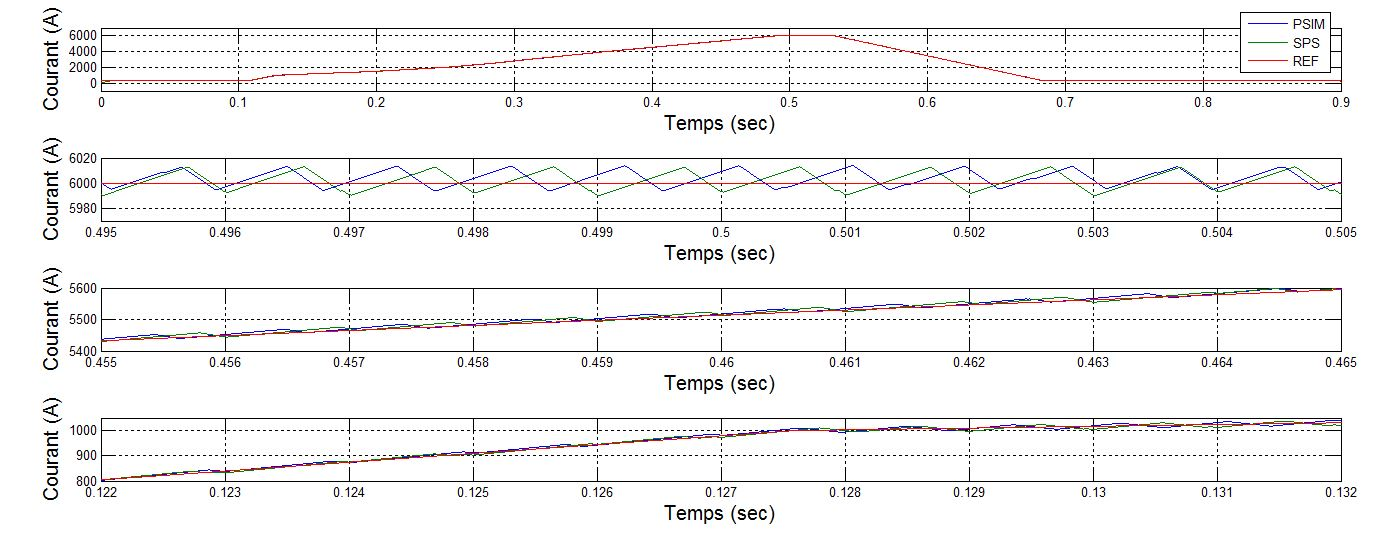
\includegraphics[scale=0.5]{fig/DCPDCN/DCPCourantCharge1u.jpg}
\caption{Courant traversant la charge sur PSIM et SPS pour un pas de calcul de 1$\mu$s pour le DCP/DCN}
\label{DC_ch_cou_1}
\end{figure}



\begin{figure}[htb]
\centering
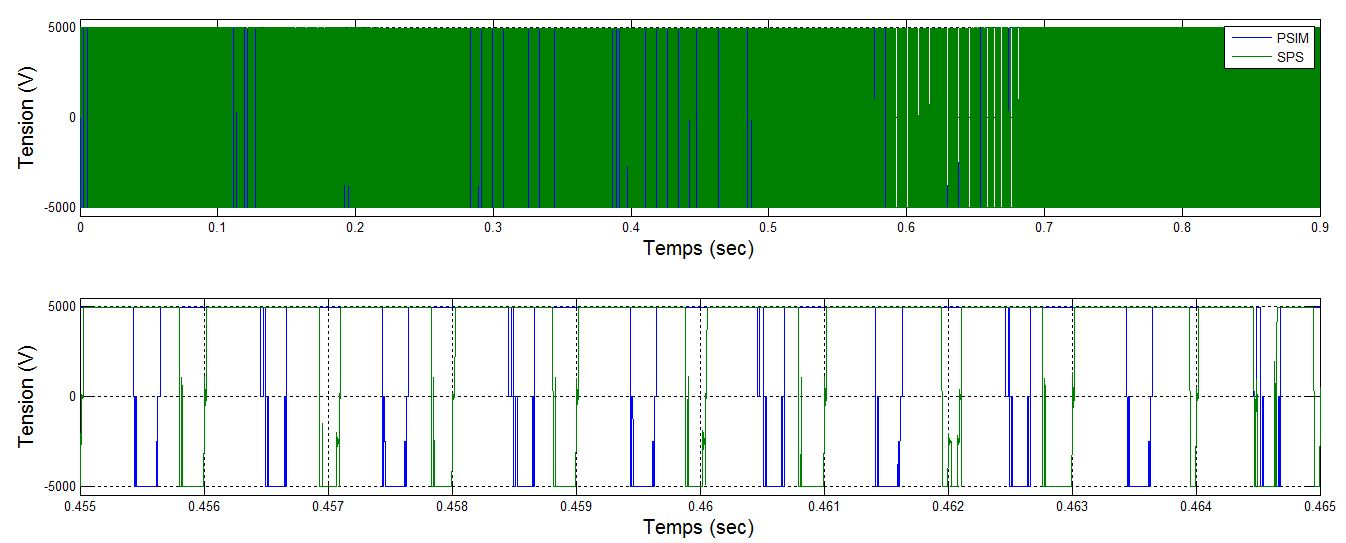
\includegraphics[scale=0.5]{fig/DCPDCN/DCPTensionCharge1u.jpg}
\caption{Tension aux bornes de la charge sur PSIM et SPS pour un pas de calcul de 1$\mu$s pour le DCP/DCN}
\label{DC_ch_ten_1}
\end{figure}


\begin{figure}[htb]
\centering
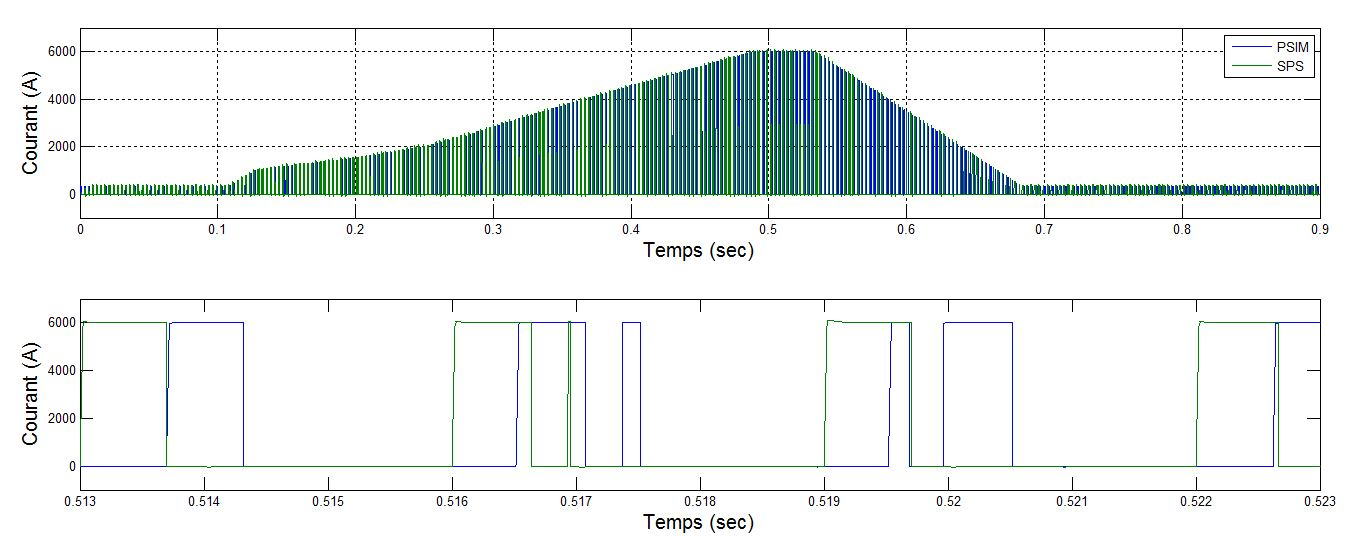
\includegraphics[scale=0.5]{fig/DCPDCN/DCPCourantIGBT1u.jpg}
\caption{Courant traversant un IGBT sur PSIM et SPS pour un pas de calcul de 1$\mu$s pour le DCP/DCN}
\label{DC_IG_cou_1}
\end{figure}


\begin{figure}[htb]
\centering
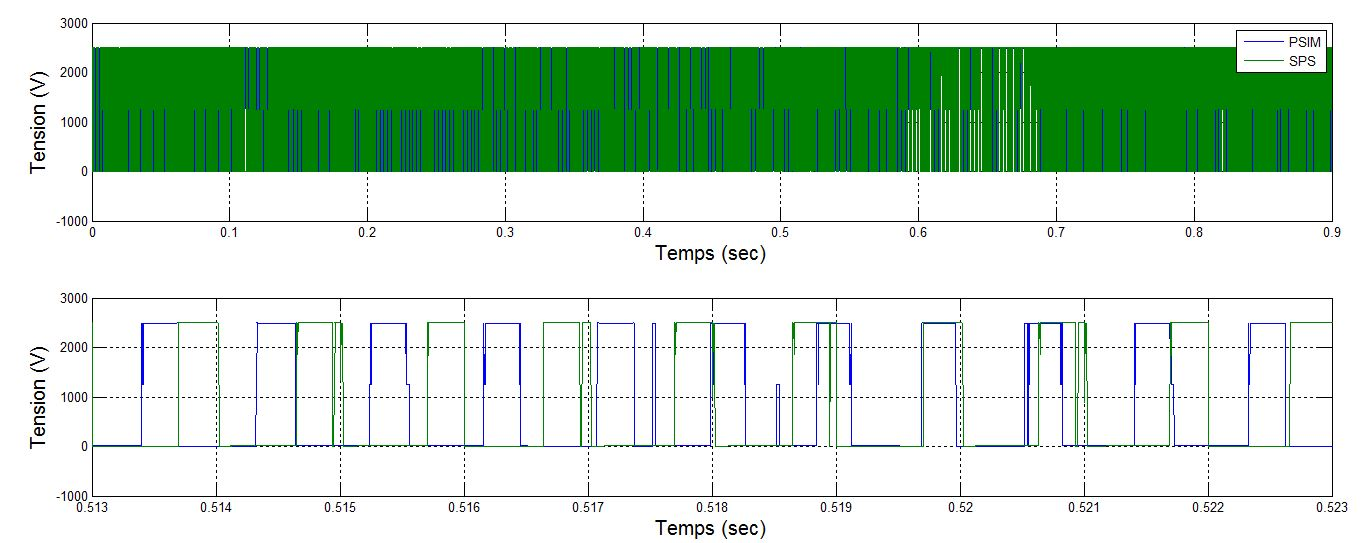
\includegraphics[scale=0.5]{fig/DCPDCN/DCPTensionIGBT1u.jpg}
\caption{Tension aux bornes d'un IGBT sur PSIM et SPS pour un pas de calcul de 1$\mu$s pour le DCP/DCN}
\label{DC_IG_ten_1}
\end{figure}


\clearpage

\subsection{Analyse des résultats comparatifs de SPS et de PSIM pour un pas de calcul de 1$\mu$s}

La figure \ref{DC_ch_cou_1} présente le courant dans la charge de manière globale , dans la zone de maintien, en montée initiale et et montée rapide. On remarque dans la figure montrant le courant dans la charge dans la zone de maintien que la fréquence de l'un des 2 simulateurs glisse par rapport à l'autre. La simulation de PSIM utilisant une analyse nodale et SPS des matrices d'équations d'états, on se doute que la détection des passages par 0 ne s'effectue pas nécessairement de manière synchrone dans les 2 simulations. De plus, la discrétisation est effectuée de manière différente dans les 2 simulations, ce qui rend les instants de détection par 0 potentiellement différents dans les 2 simulations. Les paramètres de SPS ont été réglés de manière à utiliser une méthode similaire à une méthode trapézoïdale, mais qui n'est pas nécessairement implantée de la même façon. On comprend, par rapport au hacheur 4 quadrants simple, que l'augmentation de la taille de la matrice d'équations d'états (SPS) et l'augmentation de la matrice d'admittance nodale (PSIM) permettent de constater les différences cumulatives des 2 méthodes de résolution. Les formes de courant en montée initiale et rapide montrent le même phénomène qu'en maintien, soit un glissement de la fréquence. Cependant, il est à noter que la symétrie est préservée ainsi que les amplitudes des variations.
\section{AFE 2 niveaux avec contrôle par hystérésis débitant sur une source idéale}
L'AFE (Active Front End) est un redresseur triphasé permettant de réguler le facteur de puissance à l'entrée du montage. La charge étant une source idéale pour cette simulation, il est possible d'en observer le fonctionnement dans les 4 quadrants. Ce convertisseur CA/CC est constitué de 6 interrupteurs, soit deux par bras. Ce système a pour fonction d'alimenter un bus CC et de maintenir sa tension à 5kV avec un facteur de puissance variable vu à l'entrée. Une méthode de contrôle par hystérésis est employée afin de réguler le courant (en amplitude et en phase) du côté du réseau. La figure \ref{circuit_AFE_IDEAL} présente le circuit électrique du convertisseur. Le tableau~\ref{p_AF_ID} présente les paramètres utilisés pour la simulation.

\begin{figure}[htb]
\centering
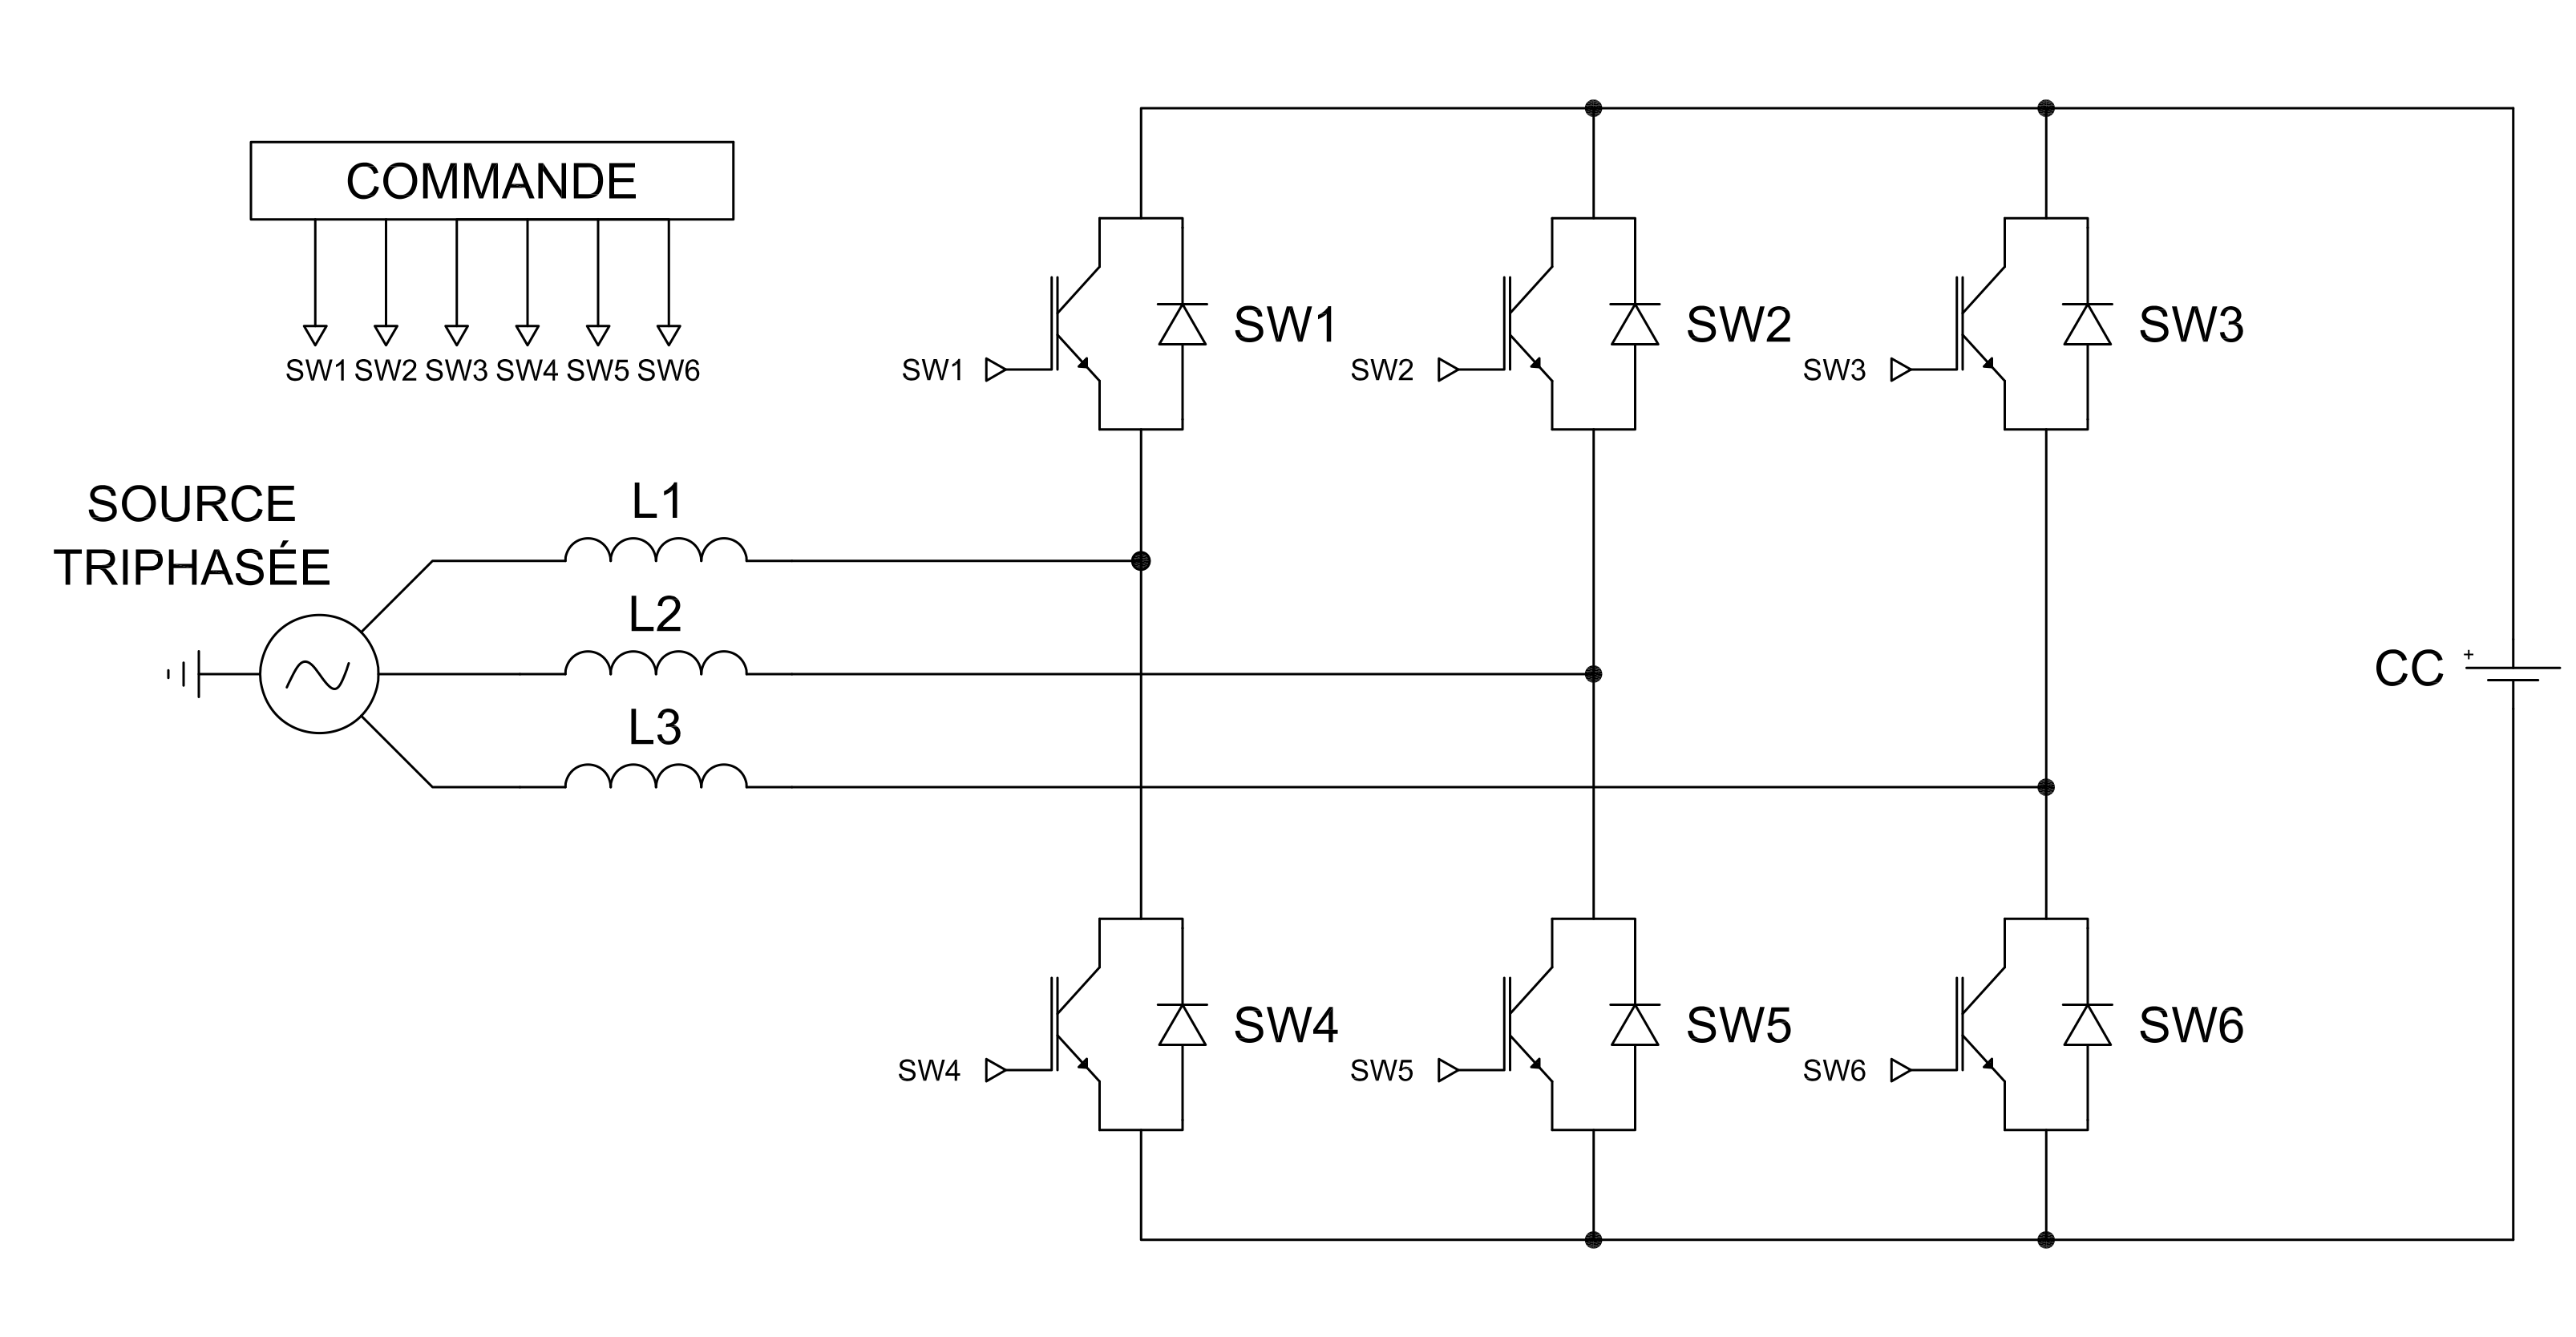
\includegraphics[scale=0.6]{fig/AFE_IDEAL.png}
\caption{Circuit électrique de l'AFE 2 niveaux sur source parfaite}
\label{circuit_AFE_IDEAL}
\end{figure}


\begin{table}[htb]
\centering
\begin{tabular}{|l|c|} 
  \hline
  \textbf{Paramètre} & \textbf{Valeur}  \\
  \hline\hline
  Tension bus CC & 5000\\ \hline
  Courant référence & 1000A\\ \hline
  Seuil hystérésis & 450A\\ \hline
  Inductance côté AC& 81.487 mH\\ \hline
  Courant maximal à l'entrée& 1500A \\ \hline \hline
  \multicolumn{2}{|l|}{\textbf{IGBT}}\\ \hline
  Résistance interne & 0.001$\Omega$\\
  Résistance du snubber & 100k$\Omega$\\ \hline \hline
   \multicolumn{2}{|l|}{\textbf{PI de courant}}\\ \hline
  Gain proportionnel & 5 \\
  Gain intégrateur & 20 \\ \hline \hline
  \multicolumn{2}{|l|}{\textbf{PI de phase}}\\ \hline
  Gain proportionnel & 0.48 \\
  Gain intégrateur & 8 \\ \hline \hline
  \hline
\end{tabular}
\caption{Paramètres de simulation pour l'AFE débitant sur une source idéale}
\label{p_AF_ID}
\end{table}
\clearpage

\subsection{Résultats de simulation pour SPS et PSIM pour un pas de calcul de 1$\mu$s}
Cette section présente les résultats de simulation de l'AFE 2 niveaux avec contrôle par hystérésis, débitant sur une source idéale, pour un pas de calcul discret de 1$\mu$s. 


\begin{figure}[htb]
\centering
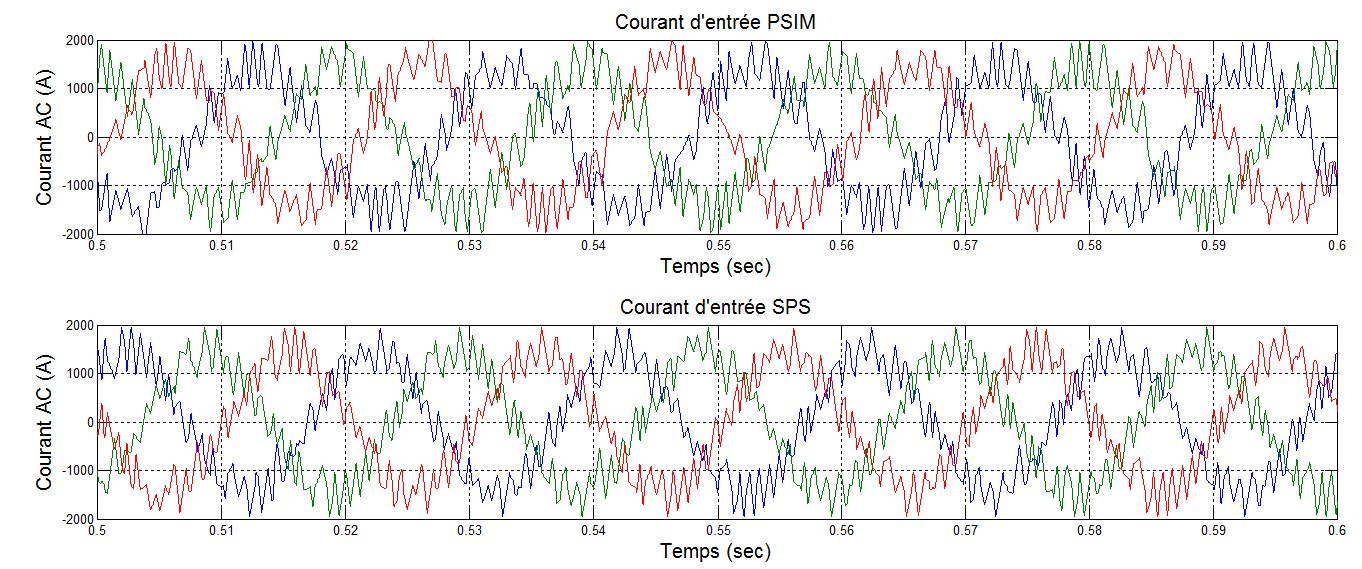
\includegraphics[scale=0.5]{fig/AFEIDEAL/CourantAC.jpg}
\caption{Le courant d'entrée avec un pas de calcul de 1$\mu$s pour l'AFE 2 niveaux avec contrôle par hystérésis sur source idéale}
\label{AF_I_cou}
\end{figure}



\begin{figure}[htb]
\centering
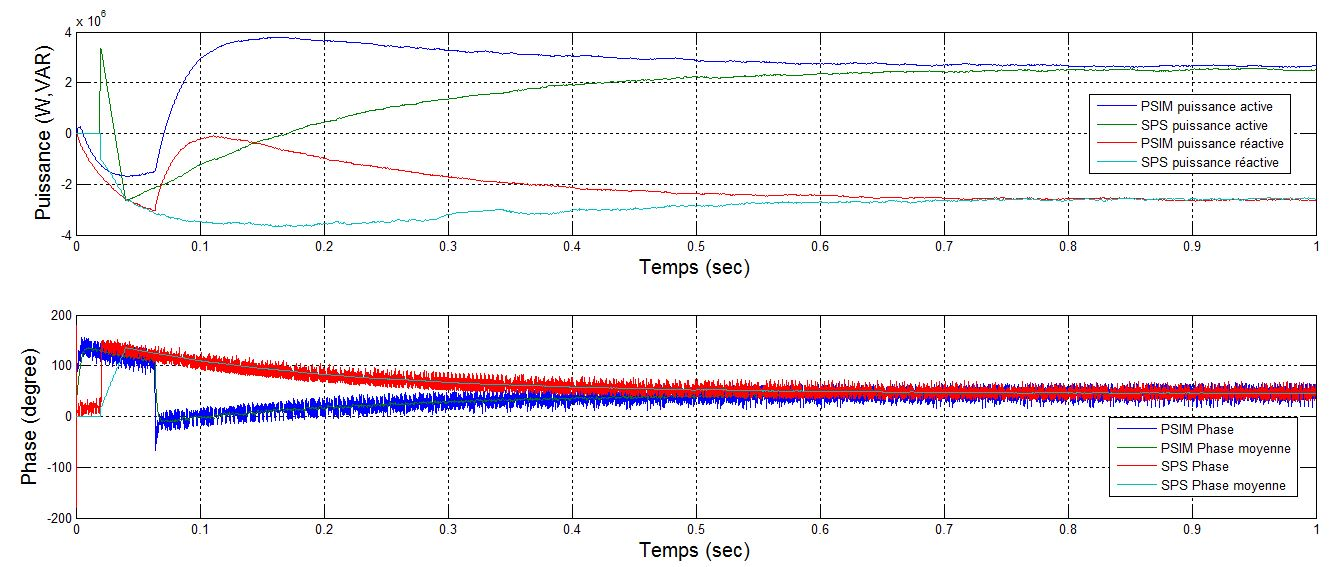
\includegraphics[scale=0.5]{fig/AFEIDEAL/pui45.jpg}
\caption{Puissances active et réactive pour une courant déphasé de 45 degré pour un pas de calcul 1$\mu$s}
\label{AF_I_pui_45}
\end{figure}

\begin{figure}[htb]
\centering
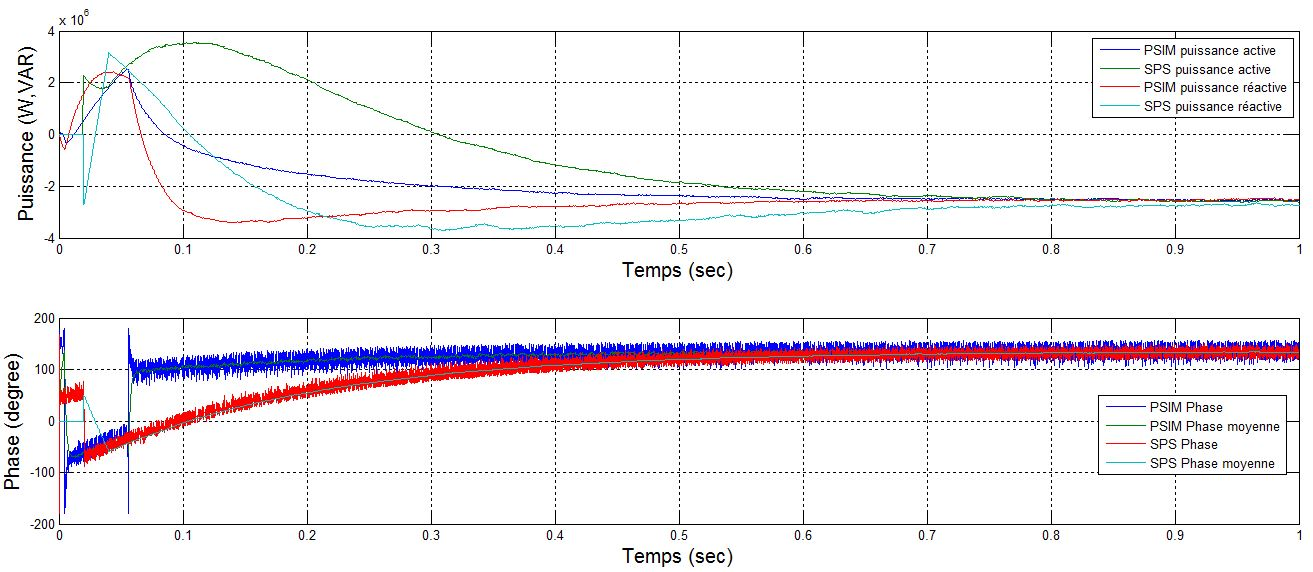
\includegraphics[scale=0.5]{fig/AFEIDEAL/pui135.jpg}
\caption{Puissances active et réactive pour une courant déphasé de 135 degré pour un pas de calcul 1$\mu$s}
\label{AF_I_pui_135}
\end{figure}

\begin{figure}[htb]
\centering
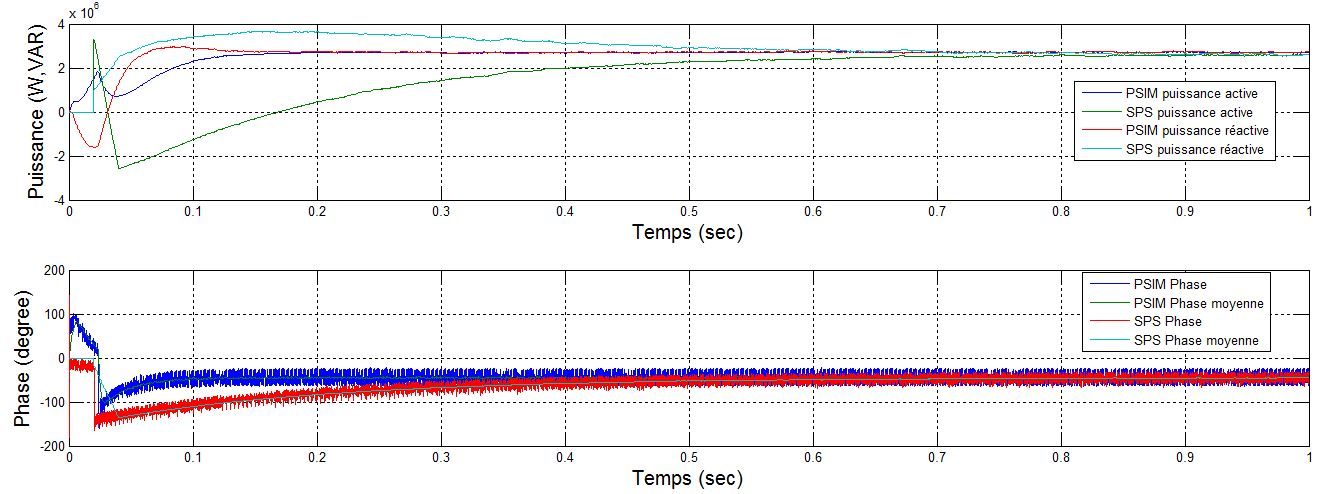
\includegraphics[scale=0.5]{fig/AFEIDEAL/pui_45.jpg}
\caption{Puissances active et réactive pour une courant déphasé de -45 degré pour un pas de calcul 1$\mu$s}
\label{AF_I_pui__45}
\end{figure}

\begin{figure}[htb]
\centering
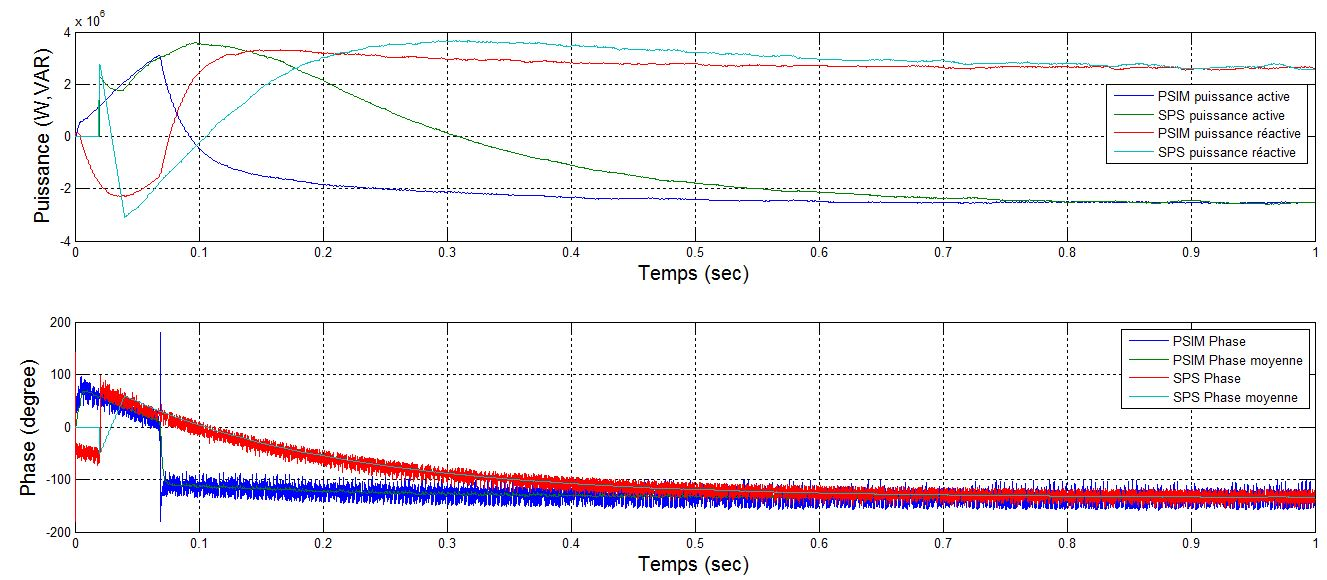
\includegraphics[scale=0.5]{fig/AFEIDEAL/pui_135.jpg}
\caption{Puissances active et réactive pour une courant déphasé de -135 degré pour un pas de calcul 1$\mu$s}
\label{AF_I_pui__135}
\end{figure}


\clearpage

\subsection{Analyse des résultats comparatifs de SPS et de PSIM pour un pas de calcul de 1$\mu$s}
La figure \ref{AF_I_cou} présente le courant à l'entrée du redresseur. On remarque que les patrons de courants sont similaires, mais qu'il existe un décalage entre les 2 simulations. Il existe des différences notables dans l'onde lorsque celle-ci dépasse une valeur angulaire de ($\pi/2$), si l'on suppose un sinus. Cette différence ainsi que le décalage s'expliquent par l'implantation de la fonction d'hystérésis qui n'est pas identique dans les 2 simulateurs. On note que les fonctions non-linéaires comme la fonction de seuillage par hystérésis sont sensibles aux méthodes de calculs et aux particularités des simulateurs. On peut le constater par la figure du courant d'entrée.

Ls figure \ref{AF_I_pui_45} présente la puissance active et réactive mesurée dans les 2 simulateurs pour une valeur d'angle imposée de 45$^\circ$ de déphasage du courant par rapport à la tension. On note rapidement que la lecture n'est précise qu'à partir d'un nombre important de cycles, l'initialisation du calcul étant intrinsèquement liés aux méthode de simulation jumelé à l'implantation du bloc dans le simulateur. La mesure de puissance implique des transformations fréquentielles ainsi que des filtres qui réduisent la dynamique du système. Les filtres employés sont sensibles au pas de calcul et peuvent présenter des différences entre les simulateurs. On note que les mesures sont lentes à comparer du procédé.

Les figures \ref{AF_I_pui_135}, \ref{AF_I_pui__45} et \ref{AF_I_pui__135} présentent la puissance active et réactive sur les 2 simulateurs pour des valeurs de déphasage de courant qui sont de 135$^\circ$, -45$^\circ$ et -135$^\circ$. Les constatations sont analogues à celles effectuées précédemment. Ces résultats montrent le fonctionnement 4 quadrant de l'AFE sur source idéale avec régulation de courant côté source et permettent de constater l'usage d'un tel dispositif, soit d'imposer le facteur de puissance vu de la source. 
\section{AFE 2 niveaux avec contrôle par hystérésis débitant sur une charge RC}
Le modèle de redresseur 2 niveaux AFE avec contrôle par hystérésis débitant sur une charge RC est le même que celui présenté à la section précédente. Le circuit du convertisseur est présenté à la figure \ref{circuit_AFE_2L_RC}. La source idéale du montage précédent est remplacée par une charge RC, composée d'une résistance de 9.26$\Omega$ et d'un condensateur initialement chargé à 5000V, d'une capacité de 330mF. De plus, contrairement au montage précédent, il n'y a plus de rétroaction sur l'angle du courant. L'angle de la référence de courant est en phase avec la tension du réseau (pour un fonctionnement à facteur unitaire). La figure \ref{fft_RC} représente le calcul de transformée de Fourier discrète (fft) d'une phase du courant d'entrée. Les paramètres de l'hystérésis ont été ajustés afin que la fréquence de commutation (qui glisse avec cette méthode de commande), soit proche de 1kHz. Le tableau \ref{p_AF_RC} présente les paramètres utilisés pour l'AFE 2 niveaux débitant sur une charge RC.

\begin{figure}[htb]
\centering
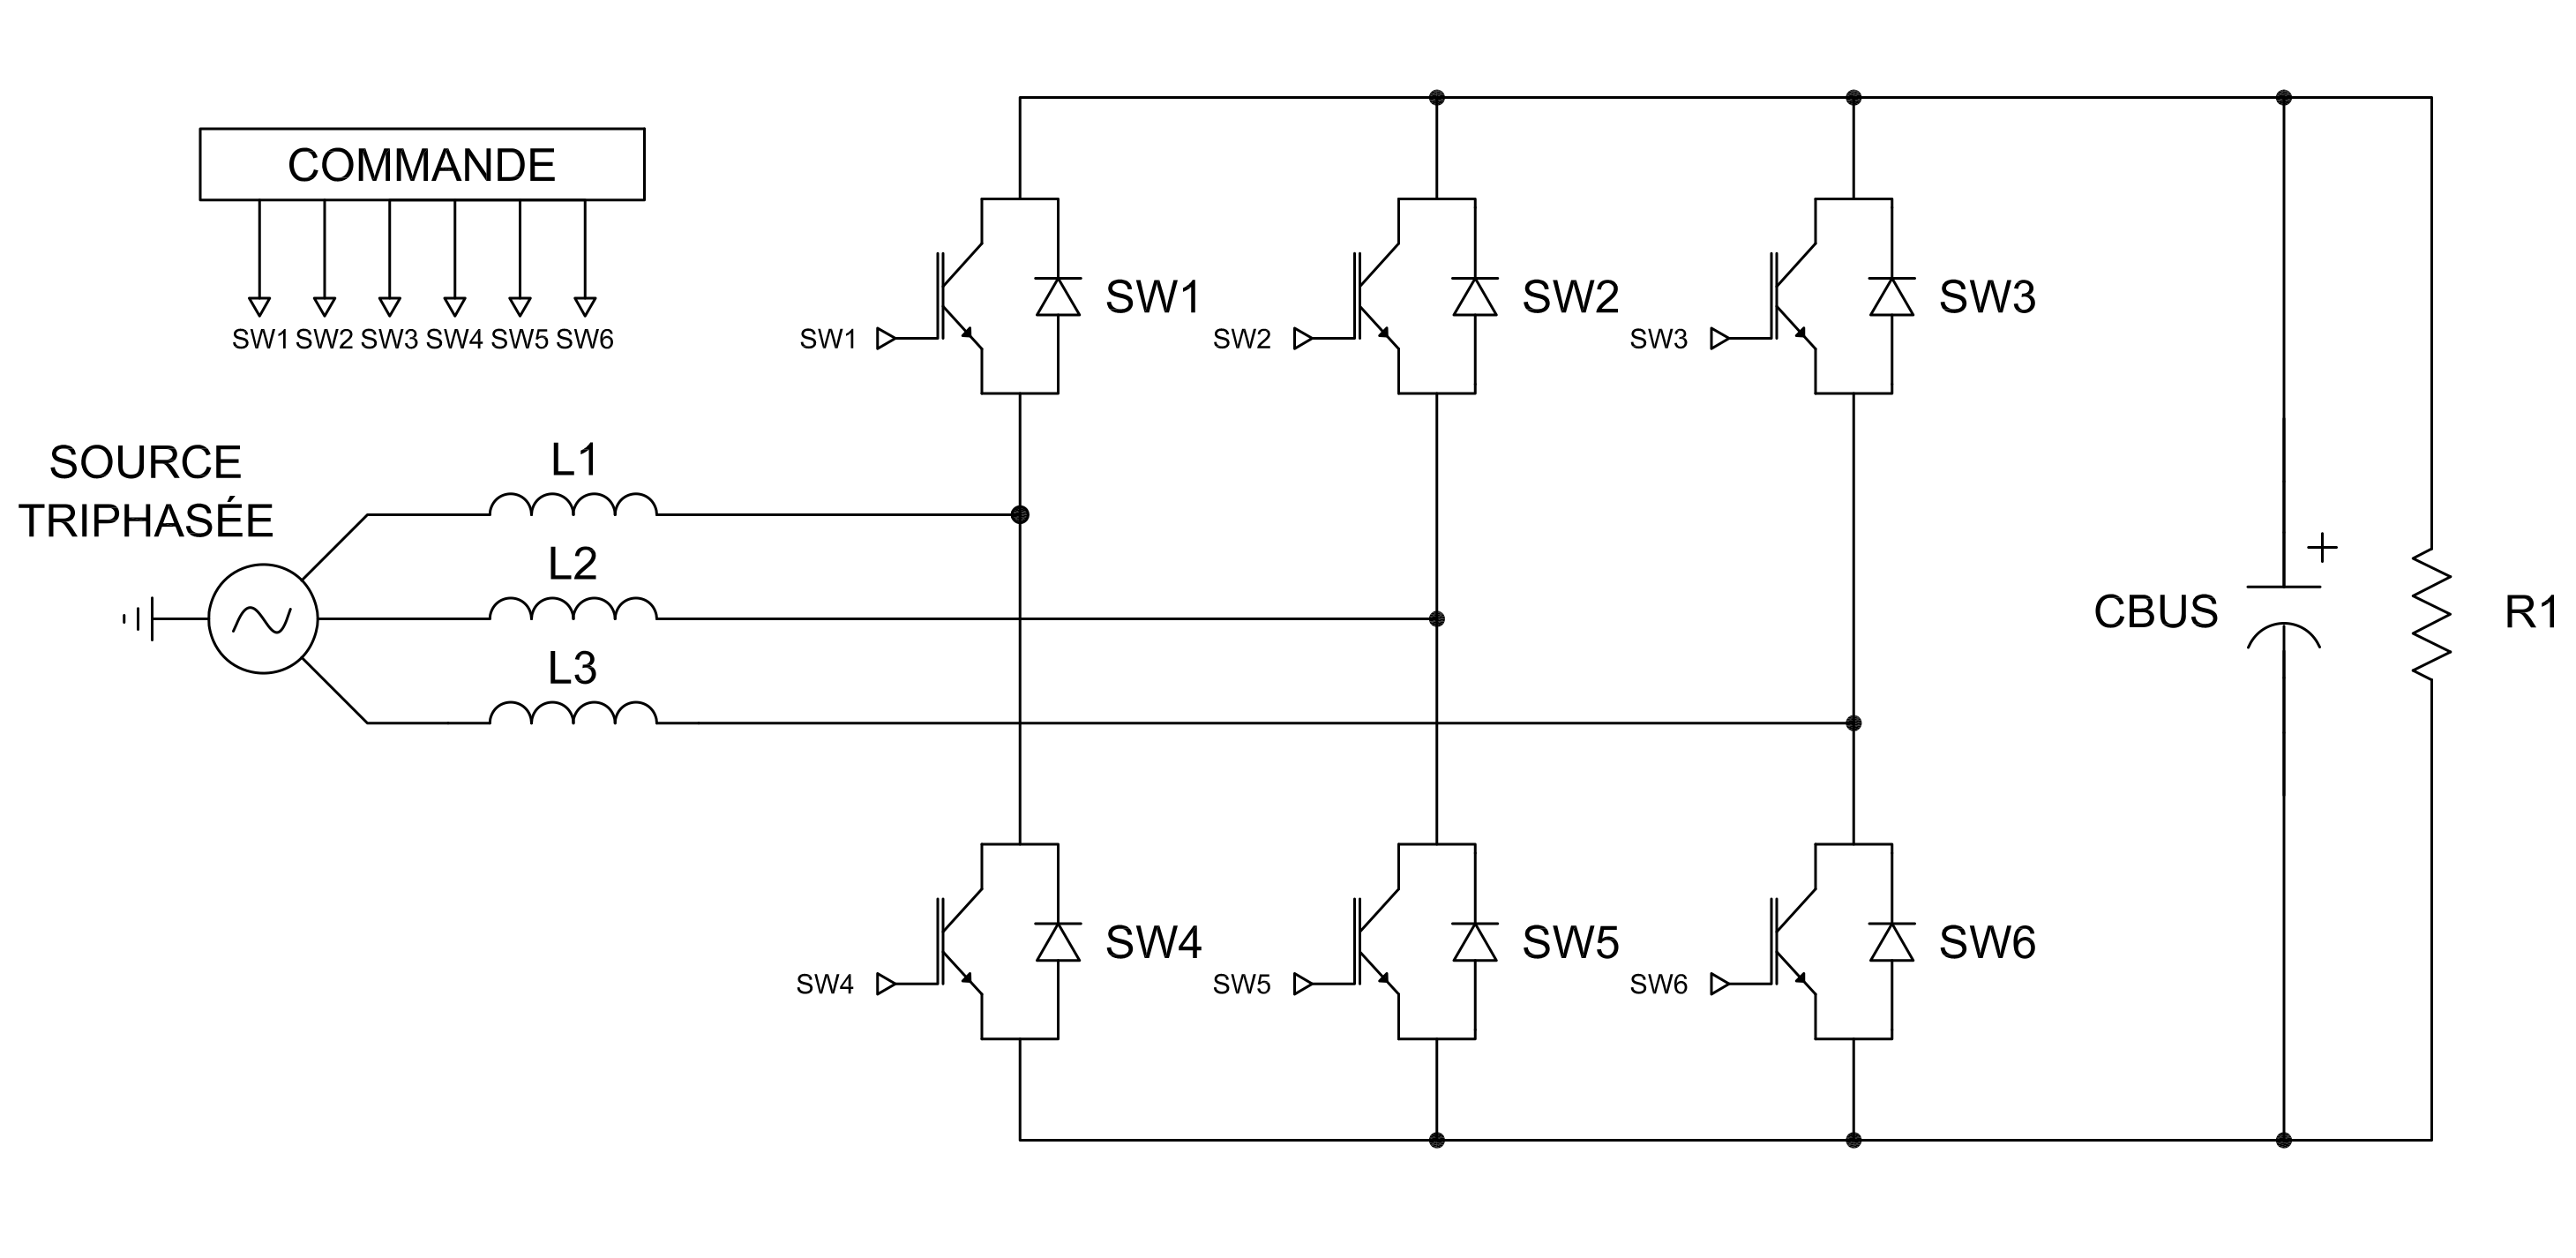
\includegraphics[scale=0.6]{fig/AFE_2L_RC.png}
\caption{Circuit électrique de l'AFE 2 niveaux sur une charge RC}
\label{circuit_AFE_2L_RC}
\end{figure}


\begin{figure}[htb]
\centering
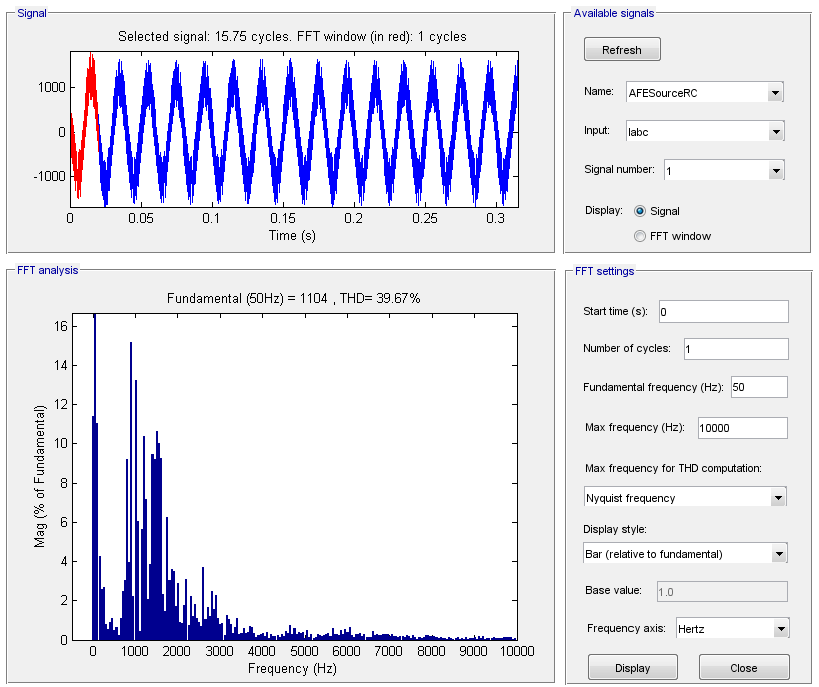
\includegraphics[scale=0.5]{fig/AFERC/FFTAnalysisToolResult5u.png}
\caption{La transformée de Fourier discrète (fft) du courant d'entrée à 1$\mu$s}
\label{fft_RC}
\end{figure}


\begin{table}[htb]
\centering
\begin{tabular}{|l|c|} 
  \hline
  \textbf{Paramètre} & \textbf{Valeur}  \\
  \hline\hline
  Tension de référence CC & 5000 V\\ \hline
  Seuil hystérésis & 450 A\\ \hline
  Inductance côté AC& 81.487 mH\\ \hline
  Courant maximal à l'entrée& 1500 A \\ \hline \hline
  \multicolumn{2}{|l|}{\textbf{IGBT}}\\ \hline
  Résistance interne & 0.001 $\Omega$\\
  Résistance du snubber & 100k $\Omega$\\ \hline \hline
   \multicolumn{2}{|l|}{\textbf{PI courant}}\\ \hline
  Gain proportionnel & 150 \\
  Gain intégrateur & 1.2e4 \\ \hline \hline
  \multicolumn{2}{|l|}{\textbf{Charge}}\\ \hline
  Résistance & 9.26 $\Omega$ \\
  Capacité d'entrée & 330 mF\\
  \hline
\end{tabular}
\caption{Paramètres de simulation pour l'AFE 2 niveaux avec contrôle par hystérésis débitant sur charge RC}
\label{p_AF_RC}
\end{table}

\clearpage

\subsection{Résultats de simulation pour SPS et PSIM pour un pas de calcul de 1$\mu$s}
Cette section présente les résultats de simulation de l'AFE 2 niveaux avec contrôle pas hystérésis sur charge RC, pour un pas de calcul discret de 1$\mu$s. 




\begin{figure}[htb]
\centering
\includegraphics[scale=0.5]{fig/AFERC/cour_al.jpg}
\caption{Le courant d'entré à 1$\mu$s pour l'AFE sur charge RC}
\label{AF_RC_cou}
\end{figure}




\begin{figure}[htb]
\centering
\includegraphics[scale=0.5]{fig/AFERC/vch.jpg}
\caption{La tension à la charge à 1$\mu$s pour l'AFE sur charge RC}
\label{AF_RC_ten}
\end{figure}



\begin{figure}[htb]
\centering
\includegraphics[scale=0.5]{fig/AFERC/IGBT.jpg}
\caption{La tension et le courant au bornes d'un IGBT à 1$\mu$s pour l'AFE sur charge RC}
\label{AF_RC_igbt}
\end{figure}

\clearpage

\subsection{Analyse des résultats comparatifs de SPS et de PSIM pour un pas de calcul de 1$\mu$s}

La figure \ref{AF_RC_cou} présente le courant à l'entrée de l'AFE pour les 2 simulateurs. Tout comme dans la section précédente, force est de constater que le comportement de l'hystérésis impact sur la qualité de l'onde dans PSIM. On remarque que le comportement dans SPS est plus régulier et permet d'obtenir un fonctionnement plus réaliste et potentiellement un glissement de fréquence de commutation (dispersion harmonique) plus faible. Les niveaux d'amplitudes sont différents en raison des surtensions dans PSIM. Le déphasage des fondamentales est moins important que dans la simulation précédente, en raison de l'absence de la régulation d'angle. 

La figure \ref{AF_RC_ten} présente la tension du bus CC en fonction du temps pour un condensateur initialement chargé. Le but est d'observer la dynamique de régulation de l'AFE, on constate que les différences sont faibles et que les 2 simulateurs fournissent un résultat similaire, malgré le courant d'entrée qui est différent.

La figure \ref{AF_RC_igbt} présente la tension et le courant d'un IGBT de l'AFE dans les 2 simulateurs. On remarque que la tension des IGBT présente des différences importantes, que l'on attribue au comportement de l'hystérésis qui détermine les temps de conduction. La forme d'onde de tension explique ce qui est observé sur l'onde de courant à l'entrée de l'AFE. Il en est de même pour l'onde de courant qui montre une plus grande régularité dans SPS.


\section{AFE 3 niveaux NPC avec contrôle par MLI}
L'AFE 3 niveaux NPC avec contrôle par MLI est composé de 12 interrupteurs IGBT ainsi que de 6 diodes de point milieu. Il représente la version finale du sous-système de l'AFE. La méthode de commande implantée diffère de celle implantée au CERN qui utilise une transformation de Park afin de simplifier le contrôle. Le circuit électrique de l'AFE 3 niveaux sur charge RC est présenté à la figure \ref{circuit_AFE_3L_RC}. Le tableau \ref{p_AF_3level} présente les paramètres utilisés avec l'AFE 3 niveaux NPC.


\begin{table}[htb]
\centering
\begin{tabular}{|l|c|} 
  \hline
  \textbf{Paramètre} & \textbf{Valeur}  \\
  \hline\hline
  Tension référence CC & 5000 V\\ \hline
  Fréquence de modulation & 1000 Hz \\ \hline
  Inductance côté AC& 81.487 mH\\ \hline
  Courant maximal à l'entrée& 800 A \\ \hline \hline
  \multicolumn{2}{|l|}{\textbf{IGBT}}\\ \hline
  Résistance interne & 0.001 $\Omega$\\
  Résistance du snubber & 100k $\Omega$\\ \hline \hline
   \multicolumn{2}{|l|}{\textbf{PI courant}}\\ \hline
  Gain proportionnel & 150 \\
  Gain intégrateur & 1.2e4 \\ \hline \hline
  \multicolumn{2}{|l|}{\textbf{PI commande}}\\ \hline
  Rapport cyclique maximal & 0.95\\
  Gain proportionnel & 1.5611 \\
  Gain intégrateur & 24.6 \\ \hline \hline
  \multicolumn{2}{|l|}{\textbf{Charge}}\\ \hline
  Résistance & 9.26 $\Omega$ \\
  Capacité d'entrée & 330 mF\\
  \hline
\end{tabular}
\caption{Paramètres de simulation pour l'AFE 3 niveaux NPC avec contrôle par MLI}
\label{p_AF_3level}
\end{table}

\begin{figure}[htb]
\centering
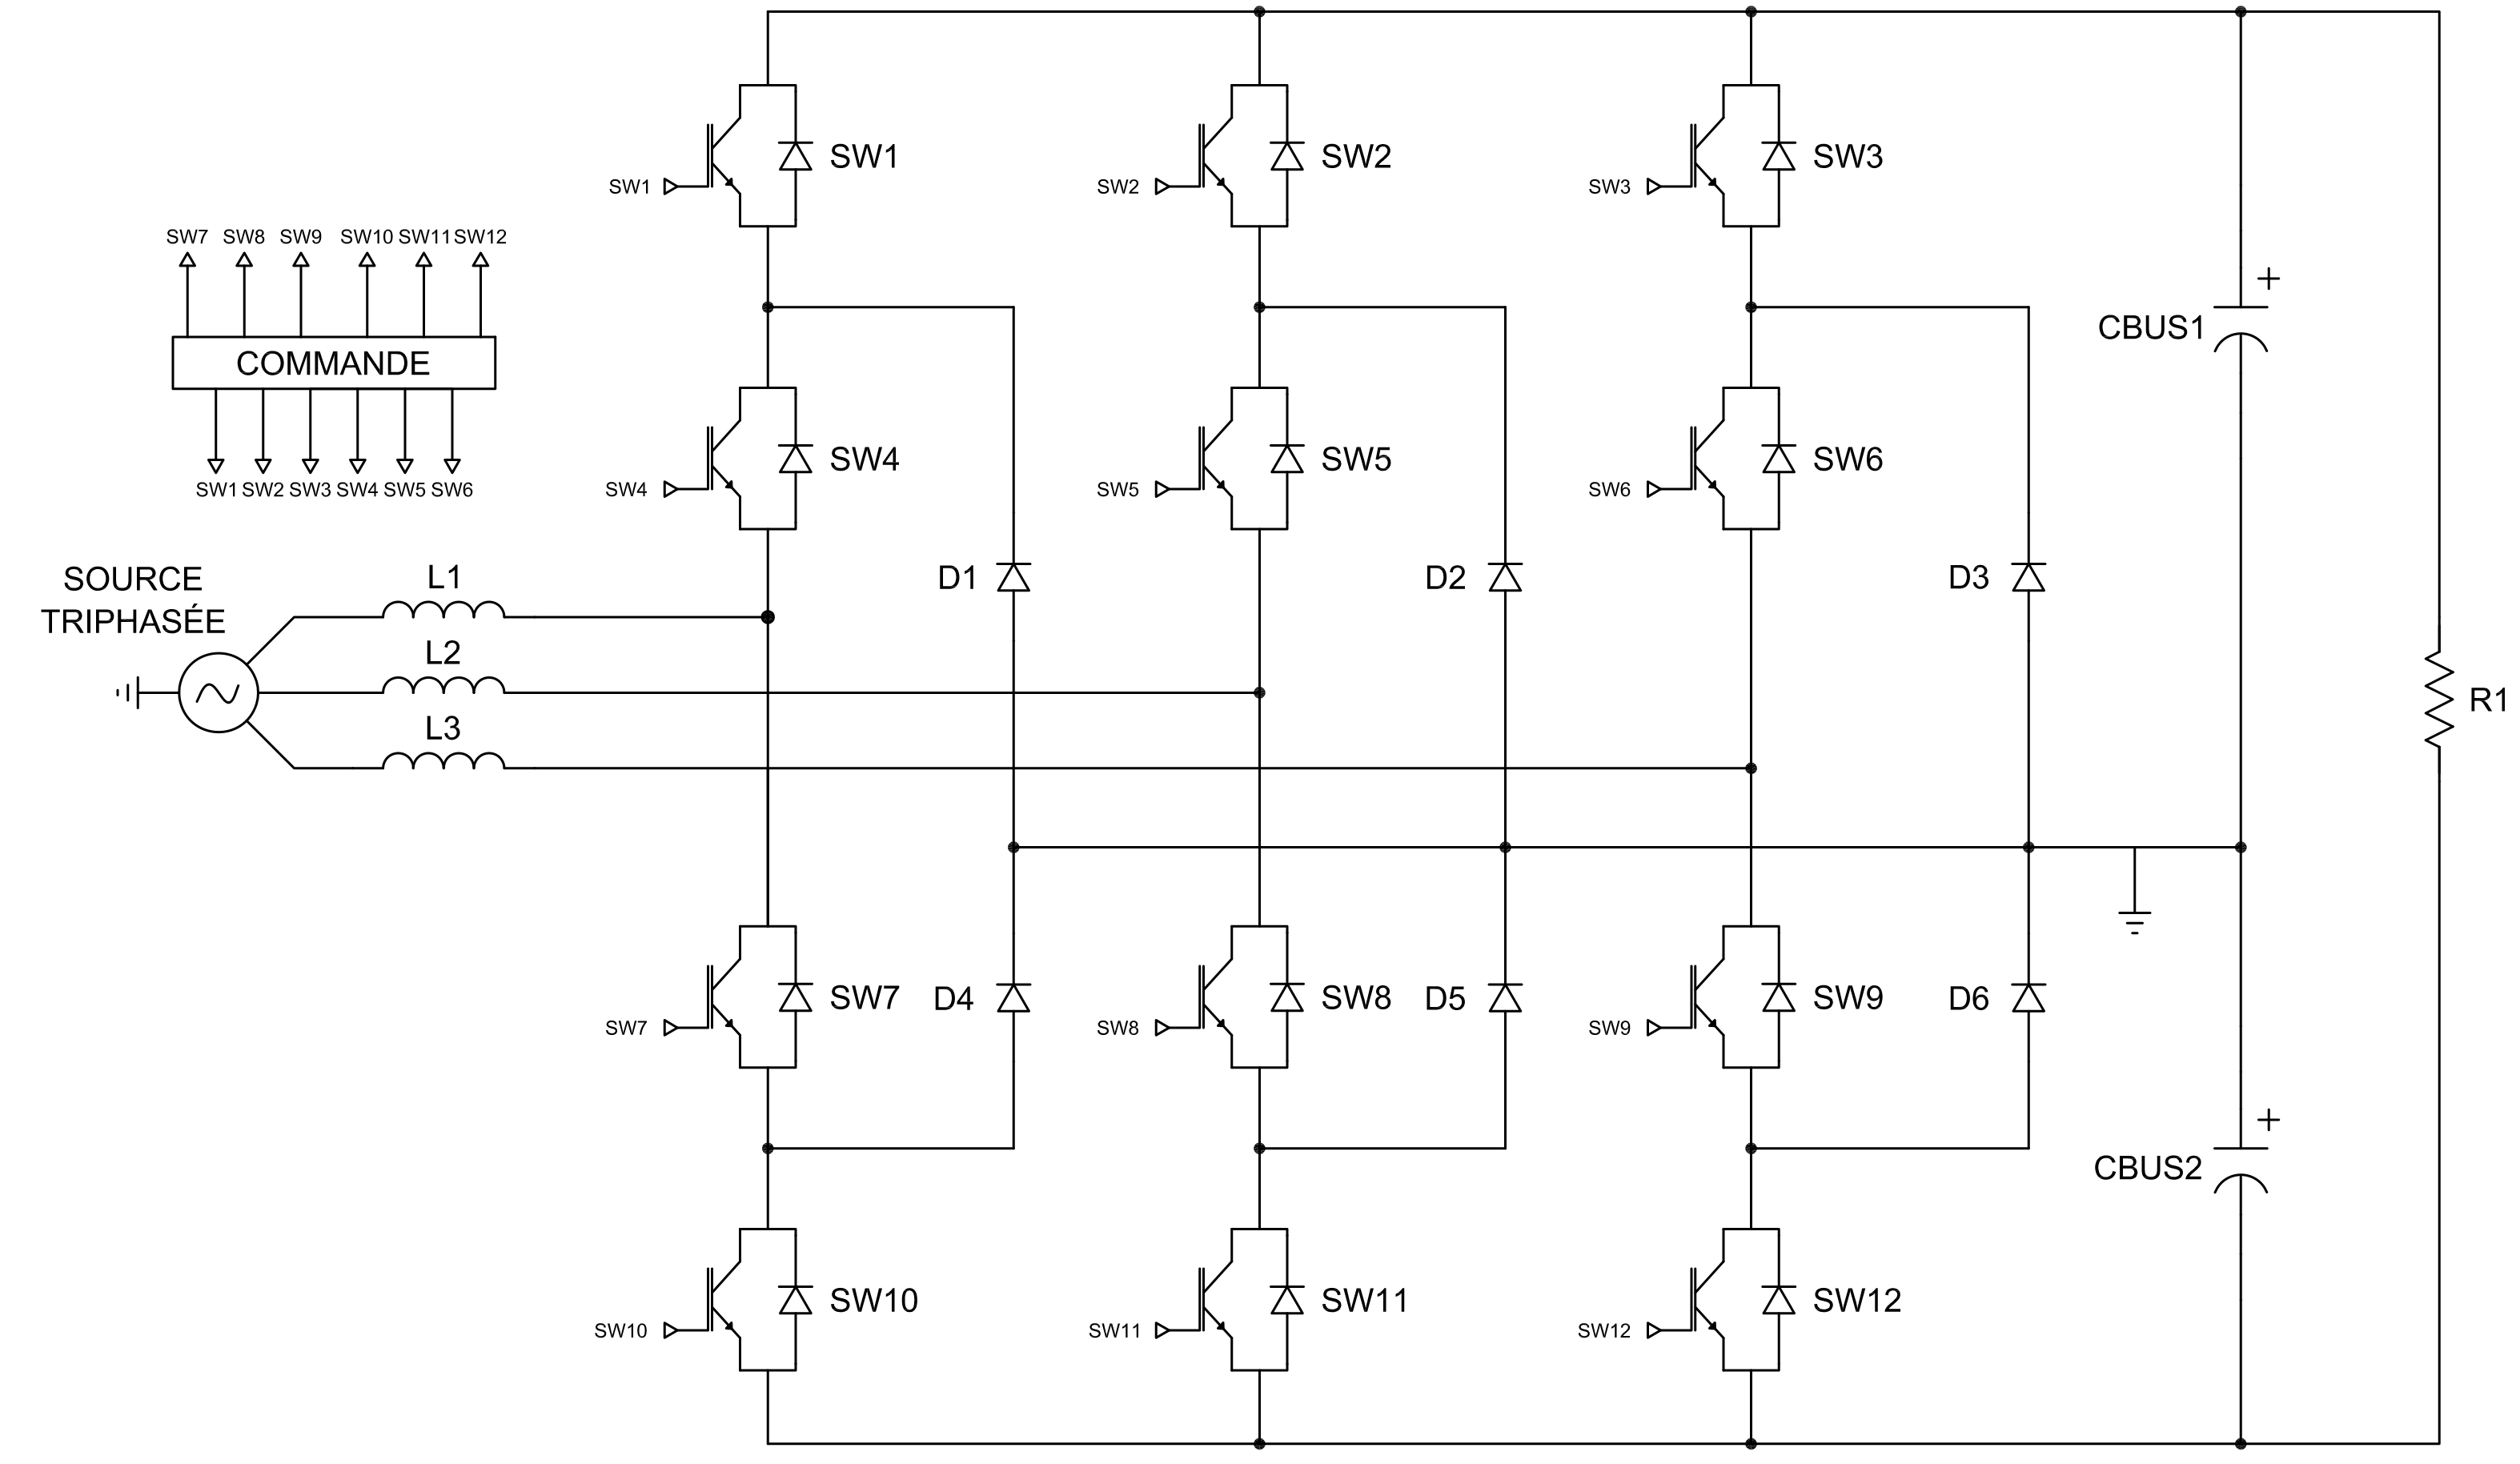
\includegraphics[scale=0.6]{fig/AFE_3L_RC.png}
\caption{Circuit électrique de l'AFE 3 niveaux sur charge RC}
\label{circuit_AFE_3L_RC}
\end{figure}


\clearpage


\subsection{Résultats de simulation pour SPS et PSIM pour un pas de calcul de 1$\mu$s}
Cette section présente les courbes d'intérêt pour la simulation de l'AFE 3 niveaux NPC avec contrôle par MLI, pour un pas de 1$\mu$s. 

\begin{figure}[htb]
\centering
\includegraphics[scale=0.5]{fig/AFE3LEVEL/1u/cour_al.jpg}
\caption{Le courant d'entrée pour un pas de calcul de 1$\mu$s, pour l'AFE 3 niveaux}
\label{AF_3_cou}
\end{figure}


\begin{figure}[htb]
\centering
\includegraphics[scale=0.5]{fig/AFE3LEVEL/1u/vch.jpg}
\caption{La tension à la charge pour un pas de calcul de 1$\mu$s, pour l'AFE 3 niveaux}
\label{AF_3_vch}
\end{figure}


\begin{figure}[htb]
\centering
\includegraphics[scale=0.5]{fig/AFE3LEVEL/1u/IGBT.jpg}
\caption{La tension et le courant au niveau d'un IGBT pour un pas de calcul de 1$\mu$s, pour l'AFE 3 niveaux}
\label{AF_3_IGBT}
\end{figure}

\begin{figure}[htb]
\centering
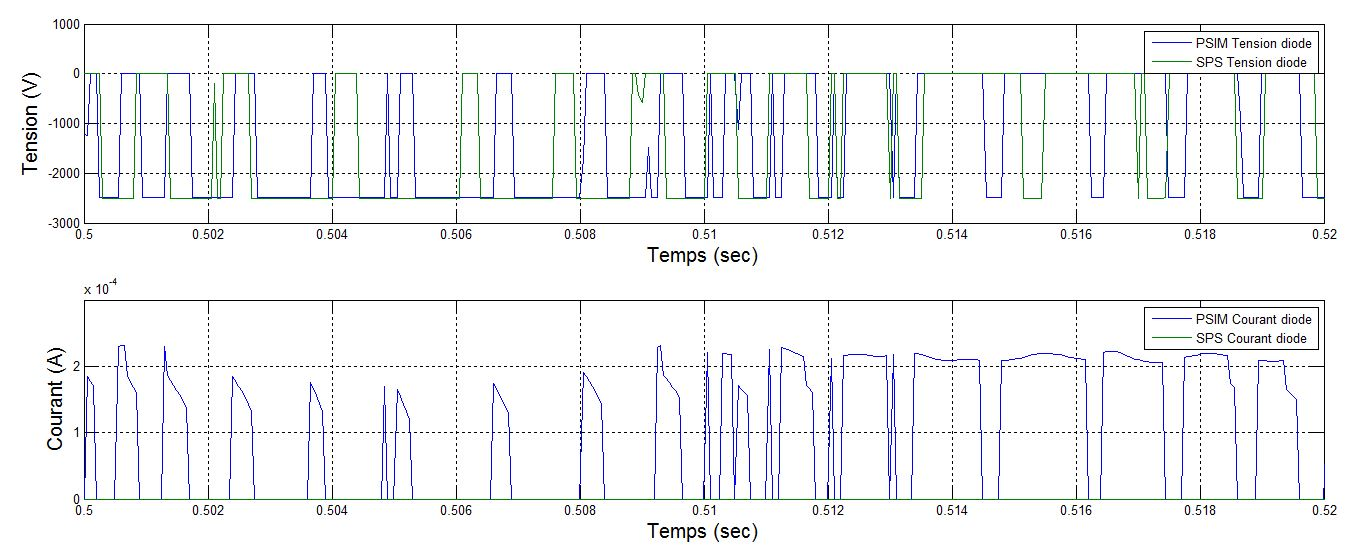
\includegraphics[scale=0.5]{fig/AFE3LEVEL/1u/DIODE.jpg}
\caption{La tension et le courant au niveau d'une diode pour un pas de calcul de 1$\mu$s, pour l'AFE 3 niveaux}
\label{AF_3_DIODE}
\end{figure}


\clearpage

\subsection{Analyse des résultats comparatifs de SPS et de PSIM pour un pas de calcul de 1$\mu$s}
La figure \ref{AF_3_cou} présente le courant d'entrée de l'AFE 3 niveaux avec contrôle par MLI. Contrairement au contrôle par hystérésis, le contrôle par MLI offre un fonctionnement beaucoup plus stable dans les 2 simulateurs. Les courbes sont pratiquement indissociable. Cela signifie que la dynamique d'implantation des PI est pratiquement identique pour les 2 simulateurs.

La figure \ref{AF_3_vch} présente la tension à la charge pour le redresseur 3 niveaux. On remarque que l'ondulation de tension est beaucoup plus faible et que les courbes sont indissociables. 

La figure \ref{AF_3_IGBT} présente la tension et le courant dans l'un des IGBT de l'AFE 3 niveaux. Contrairement à l'AFE 2 niveaux par hystérésis, on remarque une superposition des courbes et des décalages beaucoup plus faible. Les erreurs sont minimes et causées par la détection de passage par 0 qui varie suivant la méthode de solution (équations d'états ou matrice d'admittances) ainsi que selon l'algorithme de détection de passage par 0 (Tustin ou trapézoïdal pur).

La figure \ref{AF_3_DIODE} présente la tension et le courant dans l'une des diode de point milieu de l'AFE 3 niveaux. La tension aux bornes des diodes montre qu'elles s'amorcent aux mêmes instants. Les constats sont les même que ceux des IGBT sur les source d'erreur. 
\section{AFE 2 niveaux avec contrôle par hystérésis et hacheur 4 quadrants à 4 IGBT}
Cette section présente les résultat de simulations obtenus sur PSIM et SPS pour l'AFE 2 niveaux avec contrôle par hystérésis et hacheur 4 quadrants à 4 IGBT. Le circuit électronique des 2 convertisseurs est présenté à la figure \ref{circuit_H4Q_AFE_2L_RC}. Le tableau \ref{p_AF_hash} présente les paramètres utilisés dans les simulations.

\begin{figure}[htb]
\centering
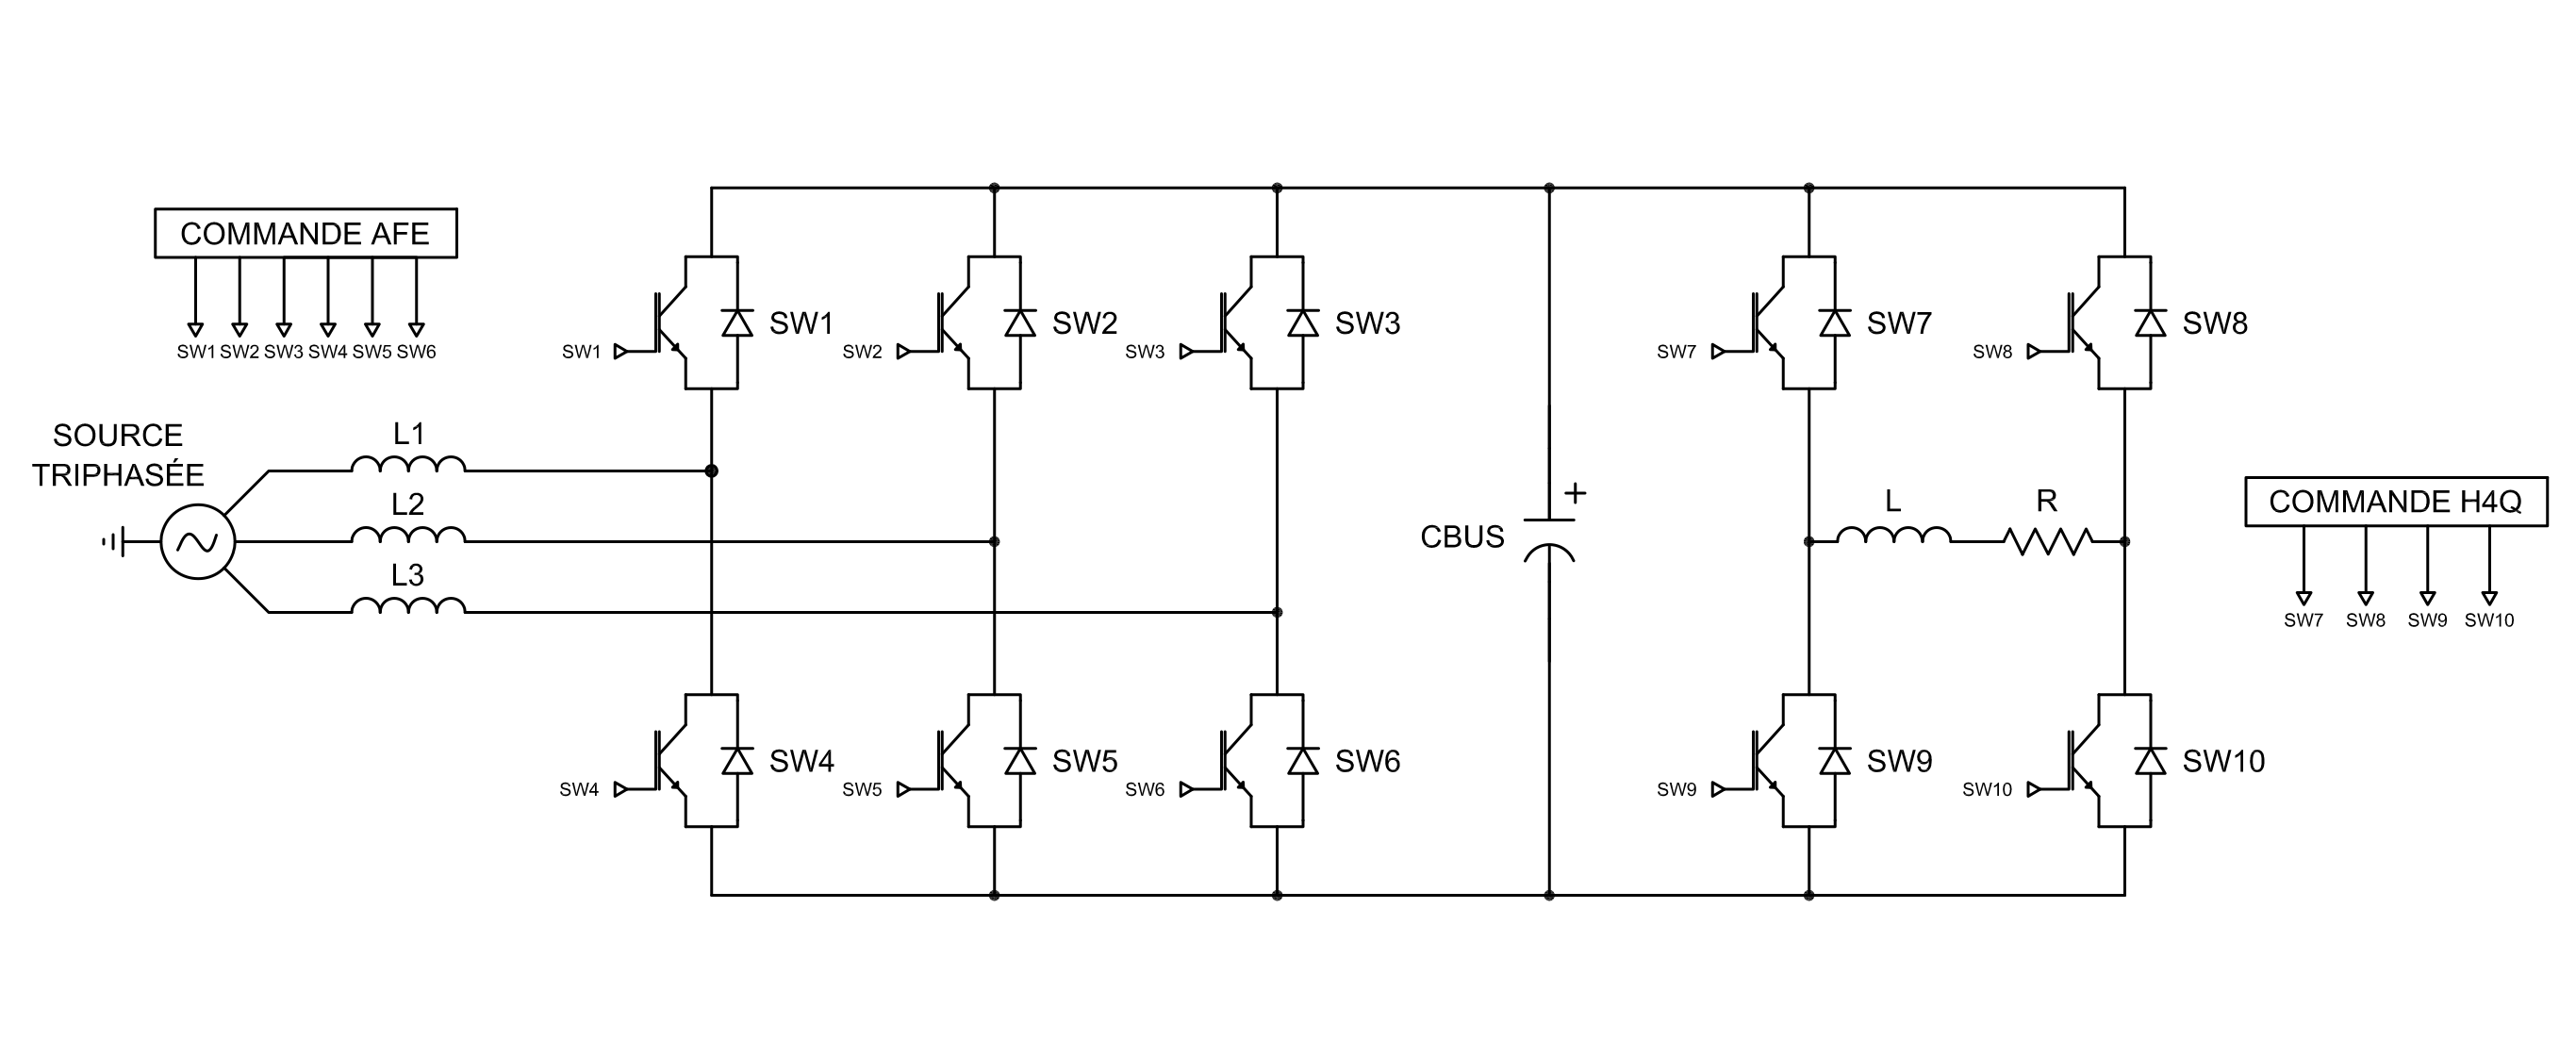
\includegraphics[scale=0.6]{fig/H4Q_AFE_2L_RC.png}
\caption{Circuit électrique de l'AFE 2 niveaux avec contrôle par hystérésis et hacheur 4 quadrants à 4 IGBT}
\label{circuit_H4Q_AFE_2L_RC}
\end{figure}


\begin{table}[htb]
\centering
\begin{tabular}{|l|c|} 
  \hline
  \textbf{Paramètre} & \textbf{Valeur}  \\
  \hline\hline \hline
  \multicolumn{2}{|l|}{\textbf{AFE 2 niveaux}}\\ \hline \hline 
  Tension référence CC & 5000 V\\ \hline
  Seuil hystérésis & 450A\\ \hline
  Inductance côté AC& 81.487 mH\\ \hline
  Courant maximal à l'entrée& 1500A \\ \hline \hline
  \multicolumn{2}{|l|}{\textbf{IGBT AFE}}\\ \hline
  Résistance interne & 0.001 $\Omega$\\
  Résistance du snubber & 100k $\Omega$\\ \hline \hline
   \multicolumn{2}{|l|}{\textbf{PI courant AFE}}\\ \hline
  Gain proportionnel & 150 \\
  Gain intégrateur & 1.2e4 \\ \hline \hline
  \multicolumn{2}{|l|}{\textbf{Bus CC}}\\ \hline
  Capacité d'entrée & 330 mF\\
  \hline \hline \hline
  
  \multicolumn{2}{|l|}{\textbf{Hacheur 4 quadrants}}\\ \hline \hline
  Fréquence de modulation & 1000 Hz\\ \hline
  Rapport cyclique maximal & 0.95 \\ \hline \hline
  \multicolumn{2}{|l|}{\textbf{IGBT hacheur}}\\ \hline
  Résistance interne & 0.001 $\Omega$\\
  Résistance du snubber & 100k $\Omega$\\ \hline \hline
   \multicolumn{2}{|l|}{\textbf{PI hacheur}}\\ \hline
  Gain proportionnel & 0.071 \\
  Gain intégrateur & 50 \\ \hline \hline
  \multicolumn{2}{|l|}{\textbf{Charge}}\\ \hline
  Résistance & 0.28 $\Omega$\\
  Inductance & 0.1 H\\
  \hline
\end{tabular}
\caption{Paramètres de simulation pour l'hacheur 4 quadrants à 4 interrupteurs avec l'AFE 2 niveaux}
\label{p_AF_hash}
\end{table}
\clearpage

\subsection{Résultats de simulation pour SPS et PSIM pour un pas de calcul de 1$\mu$s}
Cette section présente les résultats de simulation pour l'hacheur 4 quadrants à 4 interrupteurs avec l'AFE 2 niveaux sur PSIM et sur SPS, pour un pas de calcul discret de 1$\mu$s. 


\begin{figure}[htb]
\centering
\includegraphics[scale=0.5]{fig/Hach_AFE/1u/cour_al.jpg}
\caption{Le courant d'entré à 1$\mu$s section AFE}
\label{AF_HA_cou1}
\end{figure}


\begin{figure}[htb]
\centering
\includegraphics[scale=0.5]{fig/Hach_AFE/1u/ten_bus.jpg}
\caption{La tension au bus CC à 1$\mu$s section AFE}
\label{AF_HA_vch1}
\end{figure}



\begin{figure}[htb]
\centering
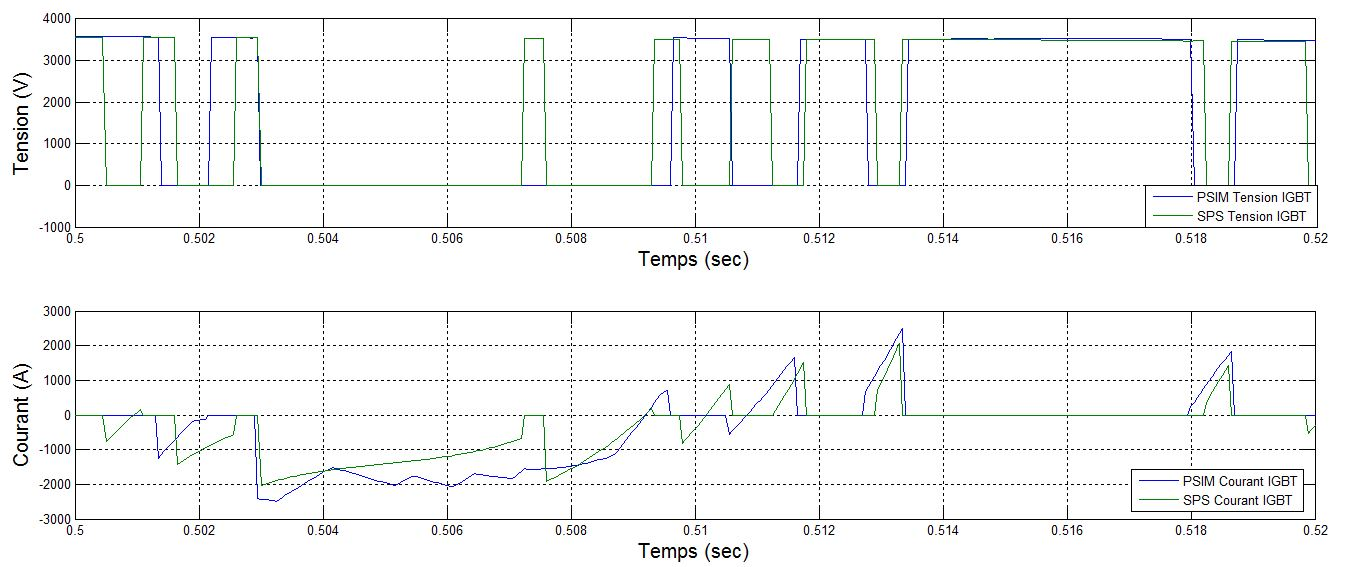
\includegraphics[scale=0.5]{fig/Hach_AFE/1u/IGBT_AFE.jpg}
\caption{La tension et le courant au niveau d'un IGBT à 1$\mu$s au niveau de l'AFE}
\label{AF_HA_IGBT1}
\end{figure}


\begin{figure}[htb]
\centering
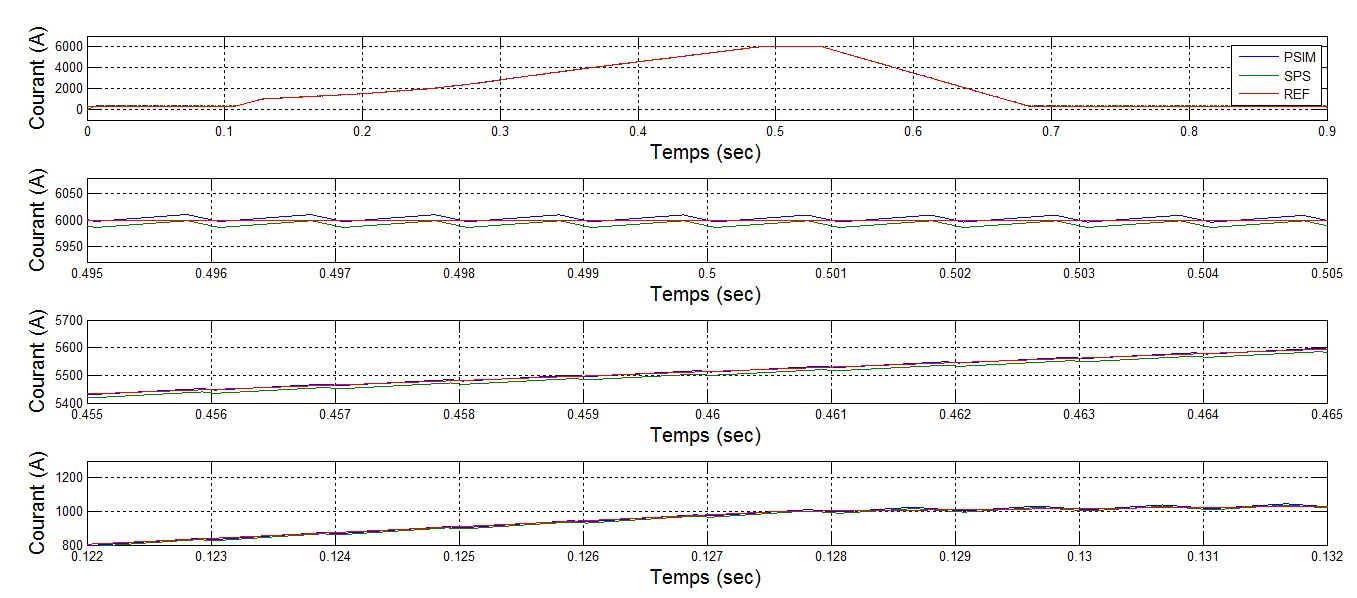
\includegraphics[scale=0.5]{fig/Hach_AFE/1u/hach_cou_ch.jpg}
\caption{Le courant au niveau de la charge à 1$\mu$s}
\label{AF_HA_CHA1}
\end{figure}



\begin{figure}[htb]
\centering
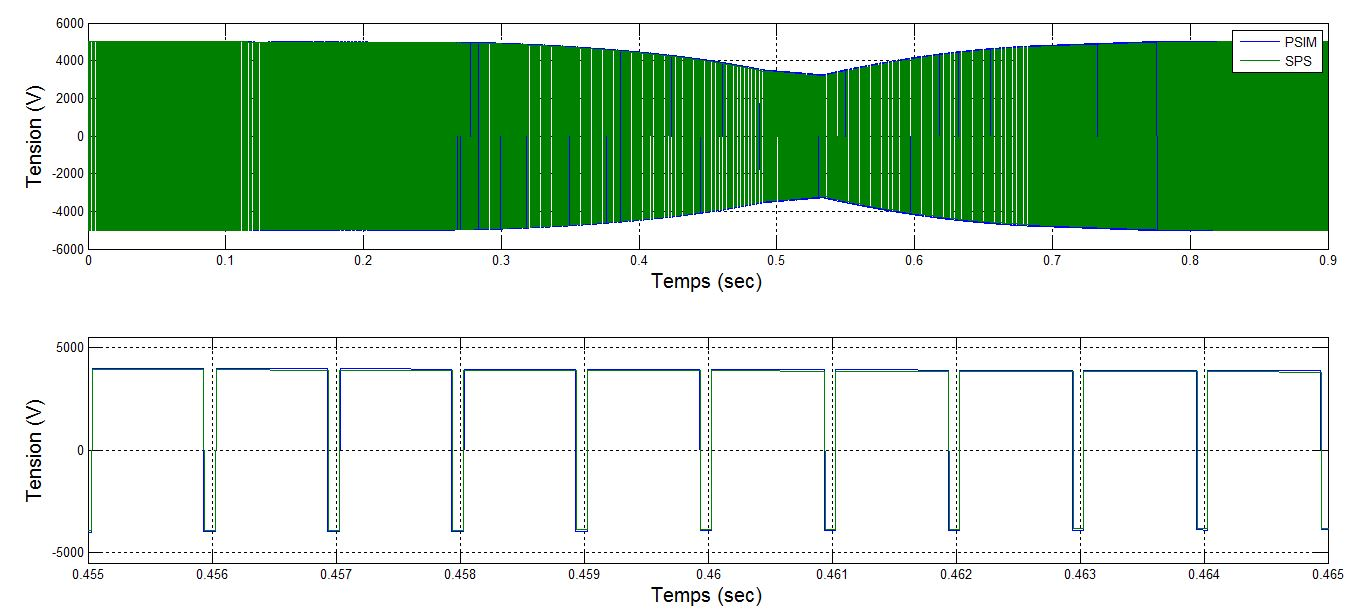
\includegraphics[scale=0.5]{fig/Hach_AFE/1u/hach_ten_ch.jpg}
\caption{La tension au niveau de la charge à 1$\mu$s}
\label{AF_HA_CHV1}
\end{figure}

\begin{figure}[htb]
\centering
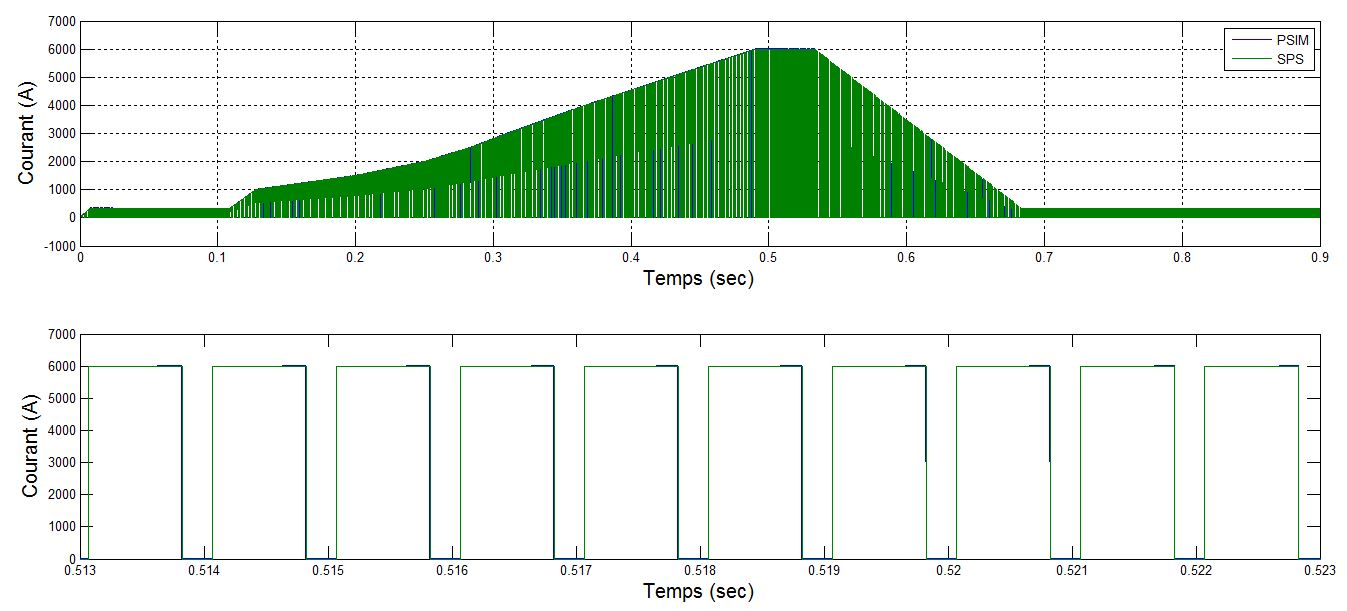
\includegraphics[scale=0.5]{fig/Hach_AFE/1u/IGBT_cou_hach.jpg}
\caption{Le courant aux bornes d'un IGBT à 1$\mu$s pour le hacheur 4 quadrants}
\label{AF_HA_HAA1}
\end{figure}

\begin{figure}[htb]
\centering
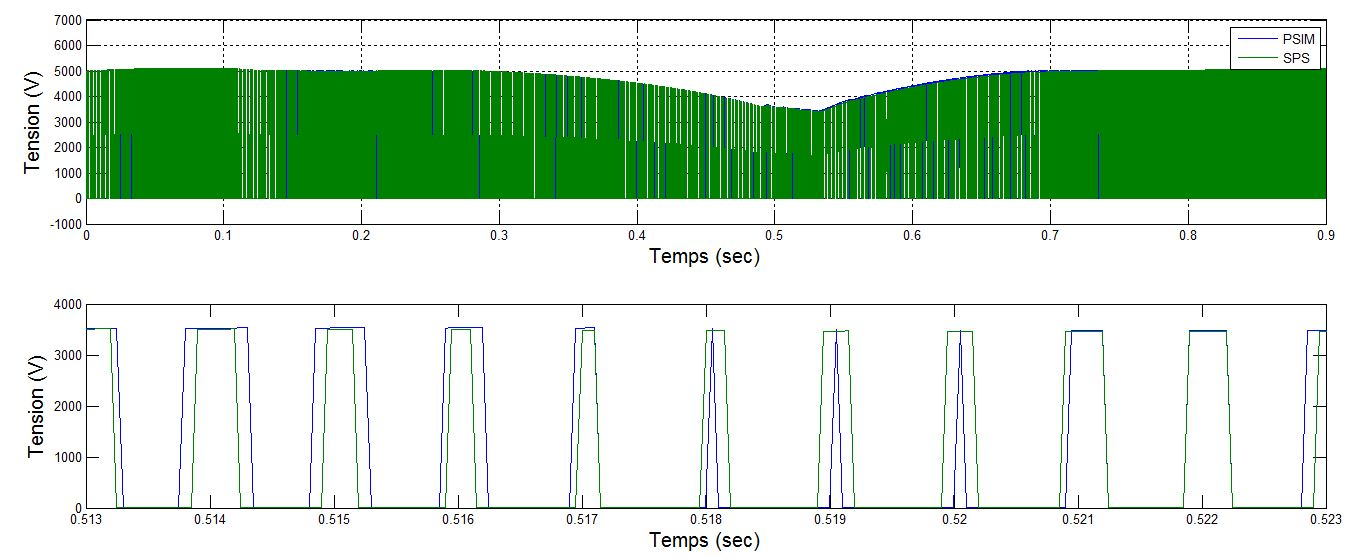
\includegraphics[scale=0.5]{fig/Hach_AFE/1u/IGBT_ten_hach.jpg}
\caption{La tension aux bornes d'un IGBT à 1$\mu$s pour le hacheur 4 quadrants}
\label{AF_HA_HAV1}
\end{figure}



\clearpage

\subsection{Analyse des résultats comparatifs de SPS et de PSIM pour un pas de calcul de 1$\mu$s}

La figure \ref{AF_HA_cou1} présente le courant d'entrée de l'AFE 2 niveaux avec contrôle par hystérésis. On remarque premièrement que les signaux sont en phases et que les amplitudes sont identiques. Cependant, l'impact des commutations sur la forme de courant diffère d'une simulation à l'autre pour les mêmes raisons qu'énoncées à la section portant sur l'AFE 2 niveaux avec controle par hystérésis sur charge RC. On remarque cependant que le fonctionnement est plus régulier.

La figure \ref{AF_DC_vch1} présente la tension du bus CC en fonction du temps pour un cycle d'alimentation des électroaimants. On remarque que les courbes ont exactement la même forme, mais qu'il y a un facteur d'échelle allant jusqu'à 200V entre les courbes. Le fonctionnement du hacheur 4 quadrants à 4 IGBT ne présentant pas de différences par rapport à celui analysé précédemment, tel qu'on peut l'observer aux figures \ref{AF_HA_CHA1} et \ref{AF_HA_CHV1}. Comme il a déjà été statué que les contrôleurs possédaient la même dynamique selon les simulateurs, il ne reste que les blocs d'hystérésis qui peuvent occasionner des différences telles que notées. La forme d'onde de courant étant différente, on se doute que la puissance instantanée est différente et qu'en contrôle dynamique, les erreurs sont cumulatives. Les hypothèses peuvent être confirmée par le courant et la tension des IGBT de l'AFE, présenté à la figure \ref{AF_HA_IGBT1}. On voit clairement les différence entre les formes de tension et de courant, ce qui confirme qu'ils ne conduisent pas aux mêmes moments. Cependant, à la figure \ref{AF_HA_HAA1} ainsi qu'à la figure \ref{AF_HA_HAV1} on constate que les interrupteurs du hacheur conduisent au mêmes moments. La preuve est donc faite que la source d'erreur apparente est inhérente aux modèles d'interrupteurs et est reliée à l'implantation de l'hystérésis du côté de l'AFE. 

\section{AFE 3 niveaux NPC avec contrôle par MLI avec convertisseur CC-CC formé de 2 cellules NPC 3 niveaux}
Cette section présente les résultats de simulations obtenus sur PSIM et sur SPS pour le système complet, formé d'un redresseur AFE 3 niveaux avec régulation MLI et d'un convertisseur CC-CC composé de 2 cellules NPC 3 niveaux.  Le circuit électronique du système complet est présenté à la figure \ref{circuit_AFE_3L_RC_DCP_DCN}. Le tableau \ref{p_AF_DCP} présente les paramètres utilisés dans les sous-systèmes.

\begin{figure}[htb]
\centering
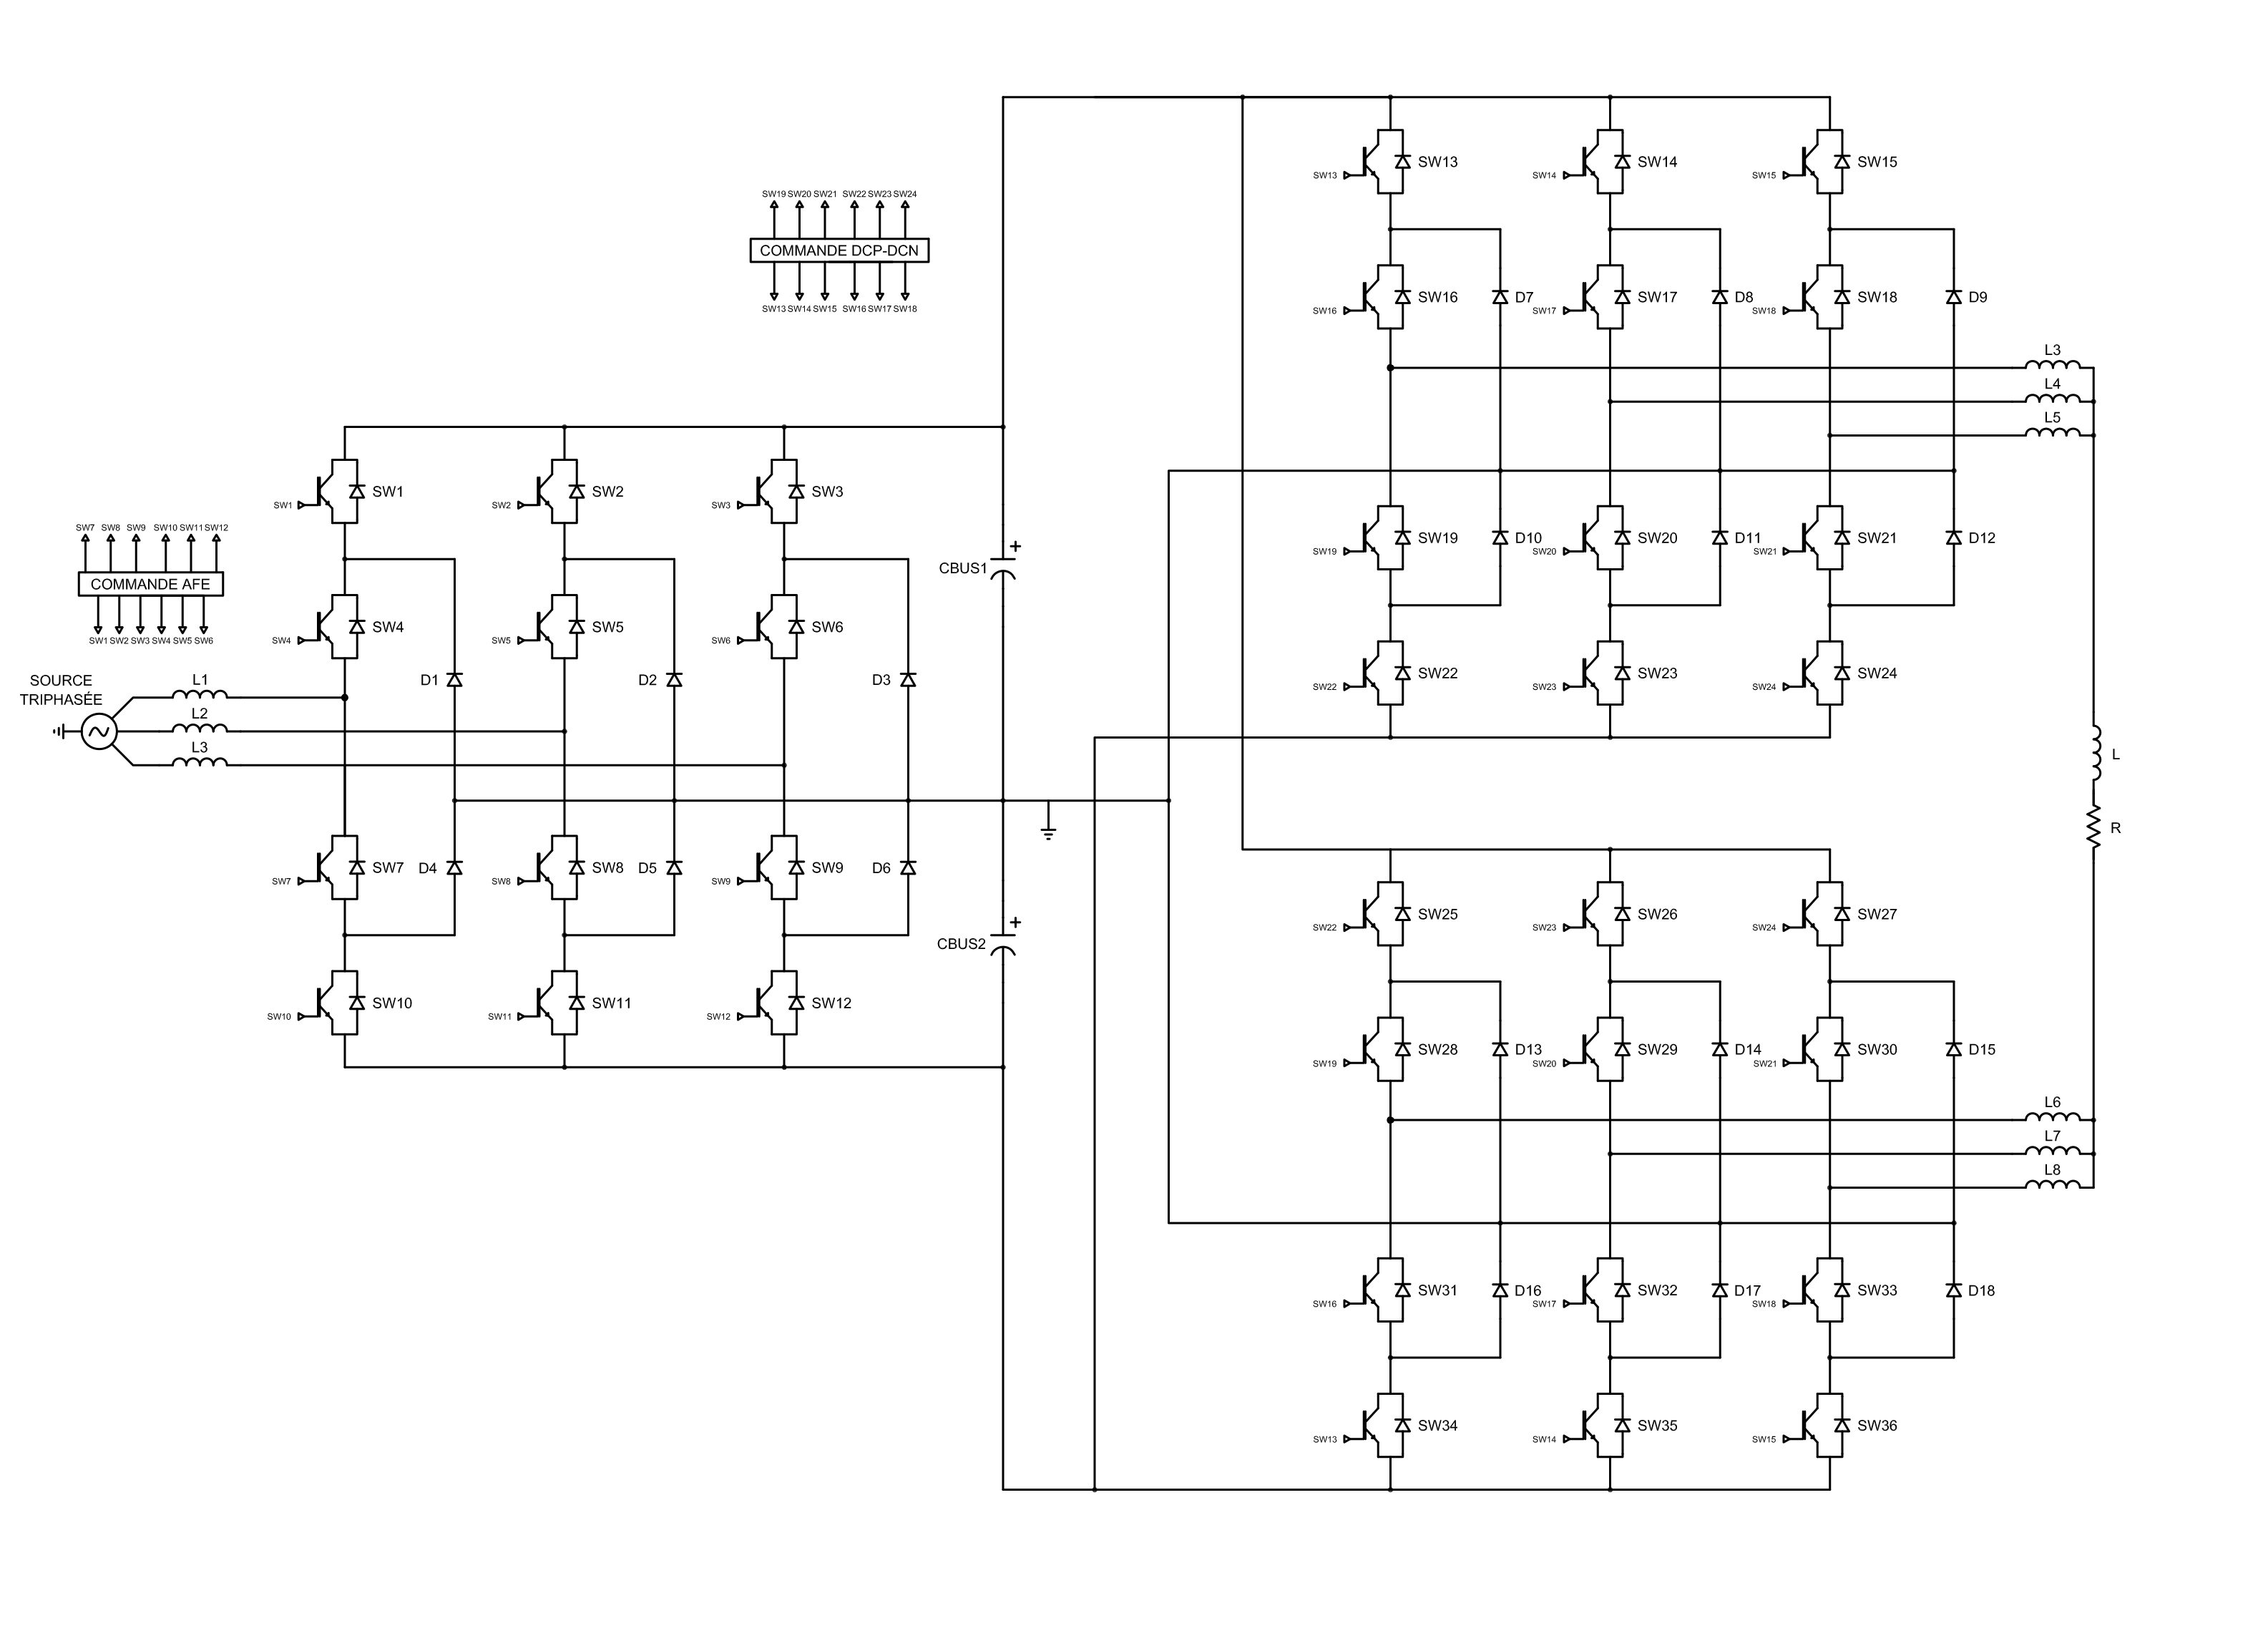
\includegraphics[scale=0.6]{fig/AFE_3L_RC_DCP_DCN.png}
\caption{Circuit électrique de l'AFE 3 niveaux avec contrôle par hystérésis avec le DCP/DCN}
\label{circuit_AFE_3L_RC_DCP_DCN}
\end{figure}


\begin{table}[htb]
\centering
\begin{tabular}{|l|c|} 
  \hline
  \textbf{Paramètre} & \textbf{Valeur}  \\
  \hline\hline \hline
  \multicolumn{2}{|l|}{\textbf{AFE 3 niveaux}}\\ \hline \hline 
  Tension référence CC & 5000 V\\ \hline
  Fréquence de modulation & 1000 Hz \\ \hline
  Inductance côté AC& 81.487 mH\\ \hline
  Courant maximal à l'entrée& 800A \\ \hline \hline
  \multicolumn{2}{|l|}{\textbf{IGBT AFE}}\\ \hline
  Résistance interne & 0.001 $\Omega$\\
  Résistance du snubber & 100k $\Omega$\\ \hline \hline
   \multicolumn{2}{|l|}{\textbf{PI courant AFE}}\\ \hline
  Gain proportionnel & 150 \\
  Gain intégrateur & 1.2e4 \\ \hline \hline
  \multicolumn{2}{|l|}{\textbf{PI commande AFE}}\\ \hline
  Rapport cyclique maximal & 0.95\\
  Gain proportionnel & 1.5611 \\
  Gain intégrateur & 24.6 \\ \hline \hline
  \multicolumn{2}{|l|}{\textbf{Bus CC}}\\ \hline
  Capacité & 330 mF\\
  \hline \hline \hline
  
  \multicolumn{2}{|l|}{\textbf{DCP/DCN}}\\ \hline \hline
  Fréquence de modulation & 333 Hz\\ \hline
  Rapport cyclique maximal & 1 \\ \hline
  Inductance de couplage & 10e-6 H \\ \hline \hline
  \multicolumn{2}{|l|}{\textbf{IGBT DCP/DCN}}\\ \hline
  Résistance interne & 0.001 $\Omega$\\
  Résistance du snubber & 100k $\Omega$\\ \hline \hline
   \multicolumn{2}{|l|}{\textbf{PI DCP/DCN}}\\ \hline
  Gain proportionnel & 1.5611 \\
  Gain intégrateur & 24.6 \\ \hline \hline
  \multicolumn{2}{|l|}{\textbf{Charge}}\\ \hline
  Résistance & 0.28 $\Omega$\\
  Inductance & 0.1 H \\
  \hline
\end{tabular}
\caption{Paramètres de simulation pour le DCP/DCN avec l'AFE 3 niveaux}
\label{p_AF_DCP}
\end{table}

\subsection{Résultats de simulation pour SPS et PSIM pour un pas de calcul de 1$\mu$s}
Cette section présente les résultats de simulations pour le système complet formé de l'AFE 3 niveaux avec régulation MLI et d'un convertisseur CC-CC composé de 2 cellules NPC 3 niveaux, pour un pas de calcul discret de 1$\mu$s. 

\begin{figure}[htb]
\centering
\includegraphics[scale=0.5]{fig/DCP_AFE/1u/cour_al.jpg}
\caption{Le courant d'entrée de l'AFE pour un pas de calcul de 1$\mu$s}
\label{AF_DC_cou1}
\end{figure}


\begin{figure}[htb]
\centering
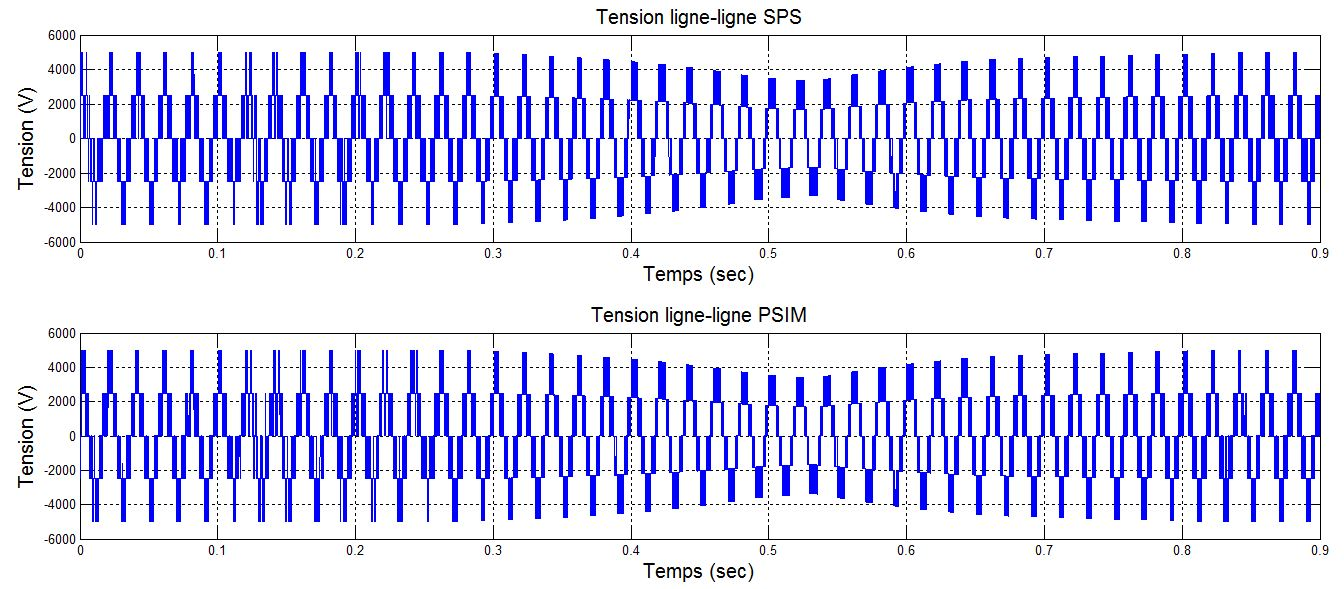
\includegraphics[scale=0.5]{fig/DCP_AFE/1u/ten_ligne_ligne.jpg}
\caption{La tension ligne-ligne d'entrée de l'AFE pour un pas de calcul de 1$\mu$s}
\label{AF_DC_ten1}
\end{figure}


\begin{figure}[htb]
\centering
\includegraphics[scale=0.5]{fig/DCP_AFE/1u/ten_bus.jpg}
\caption{La tension du bus CC pour un pas de calcul de 1$\mu$s}
\label{AF_DC_vch1}
\end{figure}



\begin{figure}[htb]
\centering
\includegraphics[scale=0.5]{fig/DCP_AFE/1u/IGBT_afe.jpg}
\caption{La tension aux bornes d'un IGBT de l'AFE pour un pas de calcul de 1$\mu$s}
\label{AF_DC_IGBT1}
\end{figure}


\begin{figure}[htb]
\centering
\includegraphics[scale=0.5]{fig/DCP_AFE/1u/cou_IGBT_afe.jpg}
\caption{Le courant aux bornes d'un IGBT de l'AFE pour un pas de calcul de 1$\mu$s}
\label{AF_DC_IGBT2}
\end{figure}


\begin{figure}[htb]
\centering
\includegraphics[scale=0.5]{fig/DCP_AFE/1u/ten_diode_afe.jpg}
\caption{La tension aux bornes d'une diode de point milieu de l'AFE à 1$\mu$s}
\label{AF_DC_DI1}
\end{figure}


\begin{figure}[htb]
\centering
\includegraphics[scale=0.5]{fig/DCP_AFE/1u/cou_diode_afe.jpg}
\caption{Le courant aux bornes d'une diode de point milieu de l'AFE à 1$\mu$s}
\label{AF_DC_DI2}
\end{figure}


\begin{figure}[htb]
\centering
\includegraphics[scale=0.5]{fig/DCP_AFE/1u/cour_ch.jpg}
\caption{Le courant aux bornes des électroaimants pour un pas de calcul de 1$\mu$s}
\label{AF_DC_CHA1}
\end{figure}



\begin{figure}[htb]
\centering
\includegraphics[scale=0.5]{fig/DCP_AFE/1u/ten_ch.jpg}
\caption{La tension aux bornes des électroaimants pour un pas de calcul de 1$\mu$s}
\label{AF_DC_CHV1}
\end{figure}



\begin{figure}[htb]
\centering
\includegraphics[scale=0.5]{fig/DCP_AFE/1u/hash_cou_IGBT.jpg}
\caption{Le courant traversant un IGBT du DCP/DCN pour un pas de calcul de à 1$\mu$s}
\label{AF_DC_HAA1}
\end{figure}



\begin{figure}[htb]
\centering
\includegraphics[scale=0.5]{fig/DCP_AFE/1u/hash_ten_IGBT.jpg}
\caption{La tension aux bornes d'un IGBT du DCP/DCN pour un pas de calcul de 1$\mu$s}
\label{AF_DC_HAV1}
\end{figure}



\begin{figure}[htb]
\centering
\includegraphics[scale=0.5]{fig/DCP_AFE/1u/hash_diode_cou.jpg}
\caption{Le courant traversant une diode de point milieu du DCP/DCN pour un pas de calcul d 1$\mu$s}
\label{AF_DC_HA1}
\end{figure}


\begin{figure}[htb]
\centering
\includegraphics[scale=0.5]{fig/DCP_AFE/1u/hash_diode.jpg}
\caption{La tension aux bornes d'une diode de point milieu du DCP/DCN pour un pas de calcul de 1$\mu$s}
\label{AF_DC_HV1}
\end{figure}


\subsection{Analyse du fonctionnement du système intégré}
Cette section correspond au point culminant du projet. La méthodologie ayant été respectée dans les précédents modèles, la construction du simulateur complet est fondée sur la compréhension acquise dans les constructions élémentaires. Ce modèle est une approximation permettant d'observer la dynamique du système comprenant des convertisseurs 3 niveaux. L'objectif ici n'est pas de documenter les sources d'erreurs, mais d'observer la dynamique globale et de comprendre les motifs liés aux contraintes physiques des systèmes implantés. La puissance traitée étant relativement élevée, les interrupteurs sont à la fois amenés à des contraintes de puissance élevées, mais aussi à des contraintes de longévité et de fiabilité. L'utilisation du modèle complet, qui est une évolution des sous-modèles présentés précédemment, permet avant tout de mettre en perspective l'impact de la charge sur le réseau qui est minimisé par l'usage d'un banc de capacité d'envergure. La pulsation de 18MW crête est fournie en grande partie par le banc de condensateur. L'AFE 3 niveaux permet à tout le moins de ramener la tension du bus à 5kV, suivant une baisse de tension causée par la demande croissante de puissance pendant la pulsation. Un AFE plus lent provoque une baisse plus marquée de la tension du bus CC, mais une perturbation moins marquée du côté du réseau. Cependant, l'atteinte du régime permanent en ce qui attrait à la tension du bus CC est plus longue et limite la fréquence des cycles. Par ailleurs, d'un point de vue économique, il est relativement plus simple d'augmenter la taille du banc de condensateurs (formés d'éléments simples) que d'utiliser des interrupteurs avec une température de jonction plus élevée. La fiabilité des interrupteurs est aussi en cause, puisqu'une augmentation de la température de jonction (causée par un appel de puissance instantanée plus grand) est néfaste pour leur durée de vie. L'objectif du système intégré est donc d'offrir un compromis entre la durée de vie des interrupteurs, le nombre de cycles répétitifs et les perturbations vues du réseau.
\subsection{Analyse des résultats comparatifs de SPS et de PSIM pour un pas de calcul de 1$\mu$s}
La figure \ref{AF_DC_cou1} présente le courant d'entrée de l'AFE débitant sur le bus CC avec le convertisseur CC-CC, formé de 2 cellules NPC 3 niveaux, en fonction. On remarque que les formes de courants sont similaires, les amplitudes pratiquement identiques et que le déphasage est minime. On en conclut donc que la méthode de modulation par MLI offre des performances, à toutes fins pratiques, identiques dans les 2 simulateurs.
La tension du bus CC est présentée à la figure \ref{AF_DC_vch1}. Sur cette figure, on remarque bien que la tension du bus CC chute pendant l'appel de puissance côté charge. On note que les 2 simulateurs réagissent de manière identique, malgré les 36 IGBT et les 18 diodes en jeu. On comprend donc que l'implantation des modèles dans les 2 simulateurs permet d'obtenir des résultats similaires. 
La figure \ref{AF_DC_ten1} présente la tension ligne-ligne vue à l'entrée de l'AFE. On constate ici la souplesse apportée par un redresseur 3 niveaux, soit un niveau intermédiaire de 2.5kV qui permet de minimiser la tension instantanée pour représenter l'onde de tension. On comprend qu'il devient alors intéressant de disposer de plusieurs niveaux afin d'être le plus près possible de la tension désirée, tout en minimisant les tensions vues aux interrupteurs.
La figure \ref{AF_DC_IGBT1} présente la tension et le courant d'un des IGBT de l'AFE. On constate que les patrons de courants sont similaires, mais que les moments d'amorçages sont différents. Le glissement est causé en grande partie, en se fiant aux constatations effectuées précédemment, par la détection des passages par 0 dans les 2 simulateurs.
La figure \ref{AF_DC_DI1} présente la tension et le courant traversant une diode de l'AFE. Tout comme dans le cas précédent, on remarque que les patrons sont similaires, mais que les moments d'amorçages sont différents et ce, pour les mêmes raisons qu'énoncées précédemment.
La figure \ref{AF_DC_CHA1} présente le courant dans la charge pendant un cycle d'impulsion, celui en montée initiale, en montée rapide et en maintien. Tout comme dans le cas du DCP/DCN, on remarque que la fréquence des oscillations de courant vues à la charge change selon les simulateurs et que les 2 signaux glissent l'un par rapport à l'autre. Les oscillations sont de même amplitude, mais elles se décalent l'une par rapport à l'autre.
Les observations pour les interrupteurs du convertisseur CC-CC sont les mêmes que celles énoncées pour l'AFE. On remarque des patrons similaires, mais des décalages en temps.


\end{document}
% Fin du document

